\documentclass[twoside,openright,10pt]{report}
%\documentclass[openright,10pt]{report}

% Package useful for debuging
%\usepackage{showlabels}

\usepackage{epsfig, supertabular, makeidx}
\usepackage{amsmath, amssymb}

% Package to add Bibliography and Index to TOC
% but not the TOC itself :-)
\usepackage[nottoc]{tocbibind}

\usepackage{hangcaption}
\usepackage{subfigure}

\usepackage{color}

% Packages needed for the cover page
\usepackage{calc, epsfig, chngpage}
\input{pstricks}\input{pst-node}\input{llnlCoverPage}

% Package useful for debuging
\usepackage{showlabels}

%----- Define some colors
\definecolor{gray}{rgb}{0.5,0.5,0.5} 

%----- Page formatting
\setlength{\oddsidemargin}{0in}
\setlength{\evensidemargin}{0in}
\setlength{\textwidth}{6.5in}
\setlength{\textheight}{8.5in}

%----- SUNDIALS MODULES
\newcommand{\sundials}{{\normalfont\scshape sundials}}
\newcommand{\nvector}{{\normalfont\scshape nvector}}
\newcommand{\nvecp}{{\normalfont\scshape nvector\_parallel}}
\newcommand{\nvecs}{{\normalfont\scshape nvector\_serial}}
\newcommand{\cvode}{{\normalfont\scshape cvode}}
\newcommand{\pvode}{{\normalfont\scshape pvode}}
\newcommand{\cvodes}{{\normalfont\scshape cvodes}}
\newcommand{\ida}{{\normalfont\scshape ida}}
\newcommand{\idas}{{\normalfont\scshape idas}}
\newcommand{\kinsol}{{\normalfont\scshape kinsol}}
\newcommand{\kinsols}{{\normalfont\scshape kinsols}}

%----- OTHER PACKAGES
\newcommand{\vode}{{\normalfont\scshape vode}}
\newcommand{\vodpk}{{\normalfont\scshape vodpk}}
\newcommand{\lsode}{{\normalfont\scshape lsode}}

%----- CVODES COMPONENTS
\newcommand{\cvdense}{{\normalfont\scshape cvdense}}
\newcommand{\cvband}{{\normalfont\scshape cvband}}
\newcommand{\cvdiag}{{\normalfont\scshape cvdiag}}
\newcommand{\cvspgmr}{{\normalfont\scshape cvspgmr}}
\newcommand{\cvbandpre}{{\normalfont\scshape cvbandpre}}
\newcommand{\cvbbdpre}{{\normalfont\scshape cvbbdpre}}
\newcommand{\stald}{{\normalfont\scshape stald}}

%----- SHARED COMPONENTS
\newcommand{\sundialsmath}{{\normalfont\scshape sundialsmath}}
\newcommand{\dense}{{\normalfont\scshape dense}}
\newcommand{\band}{{\normalfont\scshape band}}
\newcommand{\spgmr}{{\normalfont\scshape spgmr}}

%----- C and Fortran languages
\newcommand{\C}{{\sc C}}
\newcommand{\CPP}{{\sc C++}}
\newcommand{\F}{{\sc Fortran}}

%------ Serial or Parallel
\newcommand{\p}{[{\bf P}]}
\newcommand{\s}{[{\bf S}]}

%------ Appendix in text
\newcommand{\A}{App. }

%------ Index entries
\newcommand{\ID}[1]{{\tt #1}{\index{#1@\texttt{#1}|textbf}}}
\newcommand{\Id}[1]{{\tt #1}{\index{#1@\texttt{#1}}}}
\newcommand{\id}[1]{{\tt #1}}

%------ Cross reference to the user guide
\newcommand{\ugref}[1]{\ref{#1} in the user guide}

%%----- Shortcuts for math formulas
\newcommand{\mb}[1]{{\mbox{\scriptsize #1}}}
\newcommand{\dfdy}{\frac{\partial f}{\partial y}}
\newcommand{\dfdyI}{\partial f / \partial y}
\newcommand{\dfdpi}{\frac{\partial f}{\partial p_i}}
\newcommand{\dfdpiI}{\partial f / \partial p_i}
\newcommand{\rhomax}{\rho_{\max}}

%%--------------------------------
\newcommand{\frontug}
{
  \maketitle

  %% Leave an empty page
  \newpage\thispagestyle{empty}
  \vspace*{1.0in}
  
  %% Start roman numbering
  \pagestyle{plain}\pagenumbering{roman}
  \tableofcontents
  \listoftables
  \listoffigures
  
  \newpage\thispagestyle{empty}
  \vspace*{1.0in}
  
  %% Move to new page and start arabic numbering
  \newpage\pagestyle{plain}\pagenumbering{arabic}
}

%%--------------------------------
\newcommand{\frontex}
{
  \maketitle

  %% Leave an empty page
  \newpage\thispagestyle{empty}
  \vspace*{1.0in}
  
  %% Start roman numbering
  \pagestyle{plain}\pagenumbering{roman}
  \tableofcontents
  
  %% Move to new page and start arabic numbering
  \newpage\pagestyle{plain}\pagenumbering{arabic}
}

%%---------------------------------
%% Steps used in scheleton programs
%%---------------------------------
\newcounter{Stepsctr}
\newenvironment{Steps}
{\stepcounter{Stepsctr}
  \begin{list}{\arabic{Stepsctr}. }{
      \usecounter{Stepsctr}
      \setlength{\parsep}{0.5em}
      \setlength{\labelsep}{0em}
      \settowidth{\labelwidth}{99. }
      \setlength{\leftmargin}{\labelwidth+\labelsep}}}
  {\end{list}}
%%-----------------------------------------------------
%% Underlying list environemnt for function definitions
%%-----------------------------------------------------
\newenvironment{Ventry}[1][\quad]
{\begin{list}{}{
      \setlength{\rightmargin}{0em}
      \setlength{\topsep}{0.15in}
      \setlength{\itemsep}{0em}
      \renewcommand{\makelabel}[1]{##1\hfill}
      \settowidth{\labelwidth}{#1}
      \setlength{\leftmargin}{\labelwidth+\labelsep}}}
  {\end{list}}
%%----------------------------------
%% List of function arguments
%%---------------------------------
\newenvironment{args}[1][\quad]
{\begin{list}{}{
      \setlength{\rightmargin}{0em}
      \setlength{\topsep}{0em}
      \setlength{\itemsep}{0em}
      \renewcommand{\makelabel}[1]{\id{##1}\hfill}
      \settowidth{\labelwidth}{\id{#1}}
      \setlength{\leftmargin}{\labelwidth+\labelsep}}}
  {\end{list}}
%%---------------------------------
%% User-callable function
%%---------------------------------
\newcommand{\ucfunction}[6]{
  \begin{Ventry}[Return value]
  \item[\fbox{\id{#1}}]{}
  \item[Call]{\id{#2}}
  \item[Description]{#3}
  \item[Arguments]{#4}
  \item[Return value]{#5}
  \addNotes{#6}
  \end{Ventry}
}
%%---------------------------------
%% User-supplied function
%%---------------------------------
\newcommand{\usfunction}[6]{
  \begin{Ventry}[Return value]
  \item[\fbox{\id{#1}}]{}
  \item[Definition]{\id{\begin{tabular}[t]{@{}r@{}l@{}}#2\end{tabular}}}
  \item[Purpose]{#3}
  \item[Arguments]{#4}
  \item[Return value]{#5}
  \addNotes{#6}
  \end{Ventry}
}
%%---------------------------------
\makeatletter
\long\def\addNotes#1{\def\@tempa{#1}\ifx\@tempa\empty\else\item[Notes]{#1}\fi}
\makeatother

%===============================================================

\newcommand{\cvucrl}{UCRL-SM-208108}
\newcommand{\cvdate}{November 2004}
\newcommand{\cvrelease}{v2.2.0}

\title{User Documentation for {\cvode} {\cvrelease}}
\author{
  Alan C. Hindmarsh and Radu Serban\\
  {\em Center for Applied Scientific Computing} \\
  {\em Lawrence Livermore National Laboratory}
}
\date{}

%===============================================================

\makeindex

%===============================================================

\begin{document}

%Create the LLNL Cover Page
\makeLLNLCover{\cvucrl}%                        UCRL number
{User Documentation for CVODE {\cvrelease}}%    Title on cover page
{Alan C. Hindmarsh and Radu Serban}%            Authors
{\cvdate}%                                      Date
{0in}{0in}

\frontug
\renewcommand{\chaptermark}[1]{\markboth{#1}{}}
\renewcommand{\sectionmark}[1]{\markright{\thesection\ #1}}

%===============================================================
% Introduction
%===================================================================================
\chapter{Introduction}\label{s:intro}
%===================================================================================

{\cvode} is part of a software family called {\sundials}: 
SUite of Nonlinear and DIfferential/ALgebraic equation Solvers.  
This suite consists of {\cvode}, {\kinsol}, and {\ida}, and variants of these
with sensitivity analysis capabilities.
%
%---------------------------------
\section{Historical Background}\label{ss:history}
%---------------------------------

\index{CVODE@{\cvode}!relationship to {\vode}, {\vodpk}|(}
{\F} solvers for ODE initial value problems are widespread and heavily used. 
Two solvers that have been written at LLNL in the past are {\vode} \cite{BBH:89} 
and {\vodpk} \cite{Byr:92}.
{\vode}\index{VODE@{\vode}} is a general purpose solver that includes methods for
stiff and nonstiff systems, and in the stiff case uses direct methods (full or
banded) for the solution of the linear systems that arise at each implicit
step. Externally, {\vode} is very similar to the well known solver
{\lsode}\index{LSODE@{\lsode}} \cite{RaHi:94}. {\vodpk}\index{VODPK@{\vodpk}}
is a variant of {\vode} that uses a preconditioned Krylov (iterative)
method, namely GMRES, for the solution of the linear systems. {\vodpk}
is a powerful tool for large stiff systems because it combines
established methods for stiff integration, nonlinear iteration, and
Krylov (linear) iteration with a problem-specific treatment of the
dominant source of stiffness, in the form of the user-supplied
preconditioner matrix \cite{BrHi:89}.  The capabilities of both
{\vode} and {\vodpk} have been combined in the {\C}-language package
{\cvode}\index{CVODE@{\cvode}} \cite{CoHi:96}.

At present, {\cvode} contains three Krylov methods that can be used
in conjuction with Newton iteration:
the GMRES (Generalized Minimal RESidual) \cite{SaSc:86},
Bi-CGStab (Bi-Conjugate Gradient Stabilized) \cite{Van:92}, and
TFQMR (Transpose-Free Quasi-Minimal Residual) linear iterative methods
\cite{Fre:93}.  As Krylov methods, these require almost no matrix storage
for solving the Newton equations as compared to direct methods.
However, the algorithms allow for a user-supplied preconditioner
matrix, and for most problems preconditioning is essential for an
efficient solution.
For very large stiff ODE systems, the Krylov methods are preferable over
direct linear solver methods, and are often the only feasible choice.
Among the three Krylov methods in {\cvode}, we recommend GMRES as the
best overall choice.  However, users are encouraged to compare all
three, especially if encountering convergence failures with GMRES.
Bi-CGFStab and TFQMR have an advantage in storage requirements, in
that the number of workspace vectors they require is fixed, while that
number for GMRES depends on the desired Krylov subspace size.

In the process of translating the {\vode} and {\vodpk} algorithms into
{\C}, the overall {\cvode} organization has been changed considerably.
One key feature of the {\cvode} organization is that the linear system
solvers comprise a layer of code modules that is separated from the
integration algorithm, allowing for easy modification and expansion of
the linear solver array.  A second key feature is a separate module
devoted to vector operations; this facilitated the extension to
multiprosessor environments with minimal impacts on the rest of the
solver, resulting in {\pvode}\index{PVODE@{\pvode}} \cite{ByHi:99},
the parallel variant of {\cvode}.  \index{CVODE@{\cvode}!relationship
to {\vode}, {\vodpk}|)}

\index{CVODE@{\cvode}!relationship to {\cvode}, {\pvode}|(} Recently,
the functionality of {\cvode} and {\pvode} has been combined into one
single code, simply called {\cvode}. Development of the new version of
{\cvode} was concurrent with a redesign of the vector operations
module across the {\sundials} suite. The key feature of the new
{\nvector} module is that it is written in terms of abstract vector
operations with the actual vector kernels attached by a particular
implementation (such as serial or parallel) of {\nvector}. This allows
writing the {\sundials} solvers in a manner independent of the actual
{\nvector} implementation (which can be user-supplied), as well as
allowing more than one {\nvector} module linked into an executable file.
\index{CVODE@{\cvode}!relationship to {\cvode}, {\pvode}|)}

\index{CVODE@{\cvode}!motivation for writing in C|(}
There are several motivations for choosing the {\C} language for {\cvode}.
First, a general movement away from {\F} and toward {\C} in scientific
computing is apparent.  Second, the pointer, structure, and dynamic
memory allocation features in C are extremely useful in software of
this complexity, with the great variety of method options offered.
Finally, we prefer {\C} over {\CPP} for {\cvode} because of the wider
availability of {\C} compilers, the potentially greater efficiency of {\C},
and the greater ease of interfacing the solver to applications written
in extended {\F}.
\index{CVODE@{\cvode}!motivation for writing in C|)}

\section{Changes from previous versions}

\subsection*{Changes in v2.4.0}

{\cvspbcg} and {\cvsptfqmr} modules have been added to interface with the
Scaled Preconditioned Bi-CGstab ({\spbcg}) and Scaled Preconditioned
Transpose-Free Quasi-Minimal Residual ({\sptfqmr}) linear solver modules,
respectively (for details see Chapter \ref{s:simulation}). Corresponding
additions were made to the {\F} interface module {\fcvode}.
At the same time, function type names for Scaled Preconditioned Iterative
Linear Solvers were added for the user-supplied Jacobian-times-vector and
preconditioner setup and solve functions.

\subsection*{Changes in v2.3.0}

The user interface has been further refined. Several functions used
for setting optional inputs were combined into a single one.  An optional
user-supplied routine for setting the error weight vector was added.
Additionally, to resolve potential variable scope issues, all
SUNDIALS solvers release user data right after its use. The build
systems has been further improved to make it more robust.

\subsection*{Changes in v2.2.1}

The changes in this minor {\sundials} release affect only the build system.

\subsection*{Changes in v2.2.0}

The major changes from the previous version involve a redesign of the
user interface across the entire {\sundials} suite. We have eliminated the
mechanism of providing optional inputs and extracting optional statistics 
from the solver through the \id{iopt} and \id{ropt} arrays. Instead,
{\cvode} now provides a set of routines (with prefix \id{CVodeSet})
to change the default values for various quantities controlling the
solver and a set of extraction routines (with prefix \id{CVodeGet})
to extract statistics after return from the main solver routine.
Similarly, each linear solver module provides its own set of {\id{Set}-}
and {\id{Get}-type} routines. For more details see \S\ref{ss:optional_input}
and \S\ref{ss:optional_output}.

Additionally, the interfaces to several user-supplied routines
(such as those providing Jacobians and preconditioner information) 
were simplified by reducing the number
of arguments. The same information that was previously accessible
through such arguments can now be obtained through {\id{Get}-type}
functions.

The rootfinding feature was added, whereby the roots of a set of given
functions may be computed during the integration of the ODE system.

Installation of {\cvode} (and all of {\sundials}) has been completely 
redesigned and is now based on configure scripts.


\section{Reading this User Guide}\label{ss:reading}

This user guide is a combination of general usage instructions and
specific example programs.  We expect that some readers will want to
concentrate on the general instructions, while others will refer
mostly to the examples, and the organization is intended to
accommodate both styles.

There are different possible levels of usage of {\cvode}. The most
casual user, with a small IVP problem only, can get by with reading
\S\ref{ss:ivp_sol}, then Chapter \ref{s:simulation} through
\S\ref{sss:cvode} only, and looking at examples in \cite{cvode2.4.0_ex}.
In a different direction, a more expert user with an IVP problem may want
to (a) use a package preconditioner (\S\ref{ss:preconds}), (b) supply
his/her own Jacobian or preconditioner routines (\S\ref{ss:user_fct_sim}),
(c) do multiple runs of problems of the same size (\S\ref{sss:cvreinit}), 
(d) supply a new {\nvector} module (Chapter \ref{s:nvector}), or even 
(e) supply a different linear solver module
(\S\ref{ss:cvode_org} and Chapter \ref{s:gen_linsolv}).

The structure of this document is as follows:
\begin{itemize}
\item
  In Chapter \ref{s:install} we begin with instructions for the
  installation of {\cvode}, within the structure of {\sundials}.
\item
  In Chapter \ref{s:math}, we give short descriptions of the numerical
  methods implemented by {\cvode} for the solution of initial value
  problems for systems of ODEs.
\item
  The following chapter describes the structure of the {\sundials} suite
  of solvers (\S\ref{ss:sun_org}) and the software organization of the {\cvode}
  solver (\S\ref{ss:cvode_org}). 
\item
  Chapter \ref{s:simulation} is the main usage document for {\cvode} for
  {\C} applications.  It includes a complete description of the user interface
  for the integration of ODE initial value problems.
\item
  In Chapter \ref{s:fcmix}, we describe {\fcvode}, an interface module
  for the use of {\cvode} with {\F} applications.
\item
  Chapter \ref{s:nvector} gives a brief overview of the generic
  {\nvector} module shared among the various components of
  {\sundials}, and details on the two {\nvector} implementations
  provided with {\sundials}: a serial implementation
  (\S\ref{ss:nvec_ser}) and a parallel implementation based on
  MPI\index{MPI} (\S\ref{ss:nvec_par}).
\item
  Chapter \ref{s:new_linsolv} describes the interfaces to the linear
  solver modules, so that a user can provide his/her own such module.
\item
  Chapter \ref{s:gen_linsolv} describes in detail the generic linear
  solvers shared by all {\sundials} solvers.
\item
  Finally, Chapter \ref{c:constants} lists the constants used for input to
  and output from {\cvode}.
\end{itemize}

Finally, the reader should be aware of the following notational conventions
in this user guide:  program listings and identifiers (such as \id{CVodeMalloc}) 
within textual explanations appear in typewriter type style; 
fields in {\C} structures (such as {\em content}) appear in italics;
and packages or modules, such as {\cvdense}, are written in all capitals. 
In the Index, page numbers that appear in bold indicate the main reference
for that entry.

\paragraph{Acknowledgments.}
We wish to acknowledge the contributions to previous versions of the
{\cvode} and {\pvode} codes and user guides of Scott D. Cohen \cite{CoHi:94}
and George D. Byrne \cite{ByHi:98}.


\clearemptydoublepage
%===============================================================
% SUNDIALS installation procedure
\chapter{CVODE Installation Procedure}\label{s:install}

The installation of {\cvode} is accomplished by installing the
{\sundials} suite as a whole, according to the instructions that
follow.   The same procedure applies whether or not the downloaded
file contains solvers other than {\cvode}.

The {\sundials} suite (or individual solvers) are distributed as compressed archives
(\id{.tgz}). The name of the distribution archive is of the form {\em solver}\id{-x.y.z.tgz},
where {\em solver} is one of: \id{sundials}, \id{cvode}, \id{cvodes}, \id{ida}, or \id{kinsol},
and \id{x.y.z} represents the version number (of the {\sundials} suite or of the individual solver).

To begin the installation, first uncompress and expand the sources, by issuing
\begin{verbatim}
   % tar xzf solver-x.y.z.tgz
\end{verbatim}
This will extract source files under a directory {\em solver}\id{-x.y.z}.

The installation procedure outlined below will work on commodity {\linux}/{\unix} 
systems without modification. However, users are still encouraged to carefully read 
the entire chapter before attempting to install the {\sundials} suite, in case
non-default choices are desired for compilers, compilation options, or the like.
In lieu of reading the option list below, the user may invoke the configuration
script with the help flag to view a complete listing of available options, which
may be done by issuing 
\begin{verbatim}
   % ./configure --help 
\end{verbatim}
from within the directory created above.

In the remainder of this chapter, we make the following distinctions:
\begin{itemize}

\item {\em srcdir} 

  is the directory {\em solver}\id{-x.y.z} created above; i.e., the 
  directory containing the {\sundials} sources.

\item {\em builddir}

  is the directory under which {\sundials} is built; i.e., the directory
  from within which the \id{configure} command is issued. Usually, this is the same as
  {\em srcdir}.

\item {\em instdir}

  is the directory under which the {\sundials} exported header files
  and libraries will be installed. Typically, header files are exported under a directory
  {\em instdir}\id{/include} while libraries are installed under {\em instdir}\id{/lib},
  with {\em instdir} specified with the \id{--prefix} flag to \id{configure}. 
  See \S\ref{ss:configuration_options} for more details on the installation directories, 
  including the special cases of the {\sundials} examples and the {\sundialsTB} toolbox.

\end{itemize}
{\noindent}{\warn}{\em Note}: The installation directory {\em instdir} should {\em not} be the same as
the source directory {\em srcdir}.

\vspace{0.2in}
{\noindent}The installation steps for {\sundials} can be as simple as 
\begin{verbatim}
   % tar xzf solver-x.y.z.tgz
   % cd solver-x.y.z
   % ./configure
   % make
   % make install
\end{verbatim}
in which case the {\sundials} header files and libraries are installed under \id{/usr/local/include}
and \id{/usr/local/lib}, respectively. Note that, by default, neither the example programs nor the 
{\sundialsTB} toolbox are built and installed.

If disk space is a priority, then to delete all temporary files created by building {\sundials}, issue
\begin{verbatim}
   % make clean
\end{verbatim}

To prepare the {\sundials} distribution for a new install (using, for example, different options and/or
installation destinations), issue
\begin{verbatim}
   % make distclean
\end{verbatim}

%===============================================================================

\section{Configuration options}\label{ss:configuration_options}

The installation procedure given above will generally work without modification;
however, if the system includes multiple {\mpi} implementations, then certain
configure script-related options may be used to indicate which {\mpi}
implementation should be used. Also, if the user wants to use non-default
language compilers, then, again, the necessary shell environment variables must
be appropriately redefined.
%%
The remainder of this section provides explanations of available configure script
options.


\subsection*{General options}

%%
%% General options
%%

\begin{config}
  
\item \id{--prefix=PREFIX}
  
  Location for architecture-independent files.
  
  Default: \id{PREFIX=}{/usr/local}
  
\item \id{--exec-prefix=EPREFIX}

  Location for architecture-dependent files.
  
  Default: \id{EPREFIX=}{/usr/local}

\item \id{--includedir=DIR}
  
  Alternate location for installation of header files.
  
  Default: \id{DIR=PREFIX/include}
  
\item \id{--libdir=DIR}
  
  Alternate location for installation of libraries.
  
  Default: \id{DIR=EPREFIX/lib}

\item \id{--disable-}{\em solver}

  Although each existing solver module is built by default, support for a
  given solver can be explicitly disabled using this option. 
  The valid values for {\em solver} are: \id{cvode}, \id{cvodes}, 
  \id{ida}, and \id{kinsol}.

\item \id{--enable-examples}
  
  Available example programs are {\em not} built by default. Use this option
  to enable compilation of all pertinent example programs. Upon completion of 
  the \id{make} command, the example executables will be created under solver-specific
  subdirectories of {\em builddir}\id{/examples}:
  \begin{config}
  \item {\em builddir}\id{/examples/}{\em solver}\id{/serial} : serial {\C} examples
  \item {\em builddir}\id{/examples/}{\em solver}\id{/parallel} : parallel {\C} examples
  \item {\em builddir}\id{/examples/}{\em solver}\id{/fcmix\_serial} : serial {\F} examples
  \item {\em builddir}\id{/examples/}{\em solver}\id{/fcmix\_parallel} : parallel {\F} examples
  \end{config}  
  {\em Note}: Some of these subdirectories may not exist depending upon the
  solver and/or the configuration options given.

\item \id{--with-examples-instdir=EXINSTDIR}

  Alternate location for example executables and sample output files (valid only if
  examples are enabled). Note that installtion of example files can be completely disabled
  by issuing \id{EXINSTDIR=no} (in case building the examples is desired only as a test of
  the {\sundials} libraries).

  Default: \id{DIR=EPREFIX/examples}

\item \id{--with-cppflags=ARG}

  Specify additional {\C} preprocessor flags 
  (e.g., \id{ARG=-I<include\_dir>} if necessary header files are located in
   nonstandard locations).

\item \id{--with-cflags=ARG}

  Specify additional {\C} compilation flags.

\item \id{--with-ldflags=ARG}

  Specify additional linker flags (e.g., \id{ARG=-L<lib\_dir>} if
  required libraries are located in nonstandard locations).

\item \id{--with-libs=ARG}

  Specify additional libraries to be used (e.g., \id{ARG=-l<foo>} to
  link with the library named \id{libfoo.a} or \id{libfoo.so}).

\item \id{--with-precision=ARG}

  By default, {\sundials} will define a real number (internally referred to as
  \id{realtype}) to be a double-precision floating-point numeric data type
  (\id{double} {\C}-type); however, this option may be used to build {\sundials}
  with \id{realtype} alternatively defined as a single-precision floating-point
  numeric data type (\id{float} {\C}-type) if \id{ARG=single}, or as a
  \id{long double} {\C}-type if \\ \id{ARG=extended}.

  Default: \id{ARG=double}

  {\warn}Users should {\em not} build {\sundials} with support for
  single-precision floating-point arithmetic on 32- or 64-bit systems.
  This will almost certainly result in unreliable numerical solutions.
  The configuration option \id{--with-precision=single} is intended for
  systems on which single-precision arithmetic involves at least 14 decimal
  digits.

\end{config}

%%
%% Fortran support
%%

\subsection*{Options for Fortran support}

\begin{config}

\item \id{--disable-f77}

  Using this option will disable all {\F} support. The {\fcvode},
  {\fkinsol}, {\fida}, and {\fnvector} modules will not be built,
  regardless of availability.

\item \id{--with-fflags=ARG}

  Specify additional {\F} compilation flags.

\end{config}

\noindent The configuration script will attempt to automatically determine the
function name mangling scheme required by the specified {\F} compiler, but the
following two options may be used to override the default behavior.

\begin{config}

\item \id{--with-f77underscore=ARG}

  This option pertains to the {\fcvode}, {\fkinsol}, {\fida}, and {\fnvector}
  {\F}-{\C} interface modules and is used to specify the number of underscores to
  append to function names so {\F} routines can properly link with the associated
  {\sundials} libraries. Valid values for \id{ARG} are: \id{none}, \id{one}
  and \id{two}.

  Default: \id{ARG=one}

\item \id{--with-f77case=ARG}

  Use this option to specify whether the external names of the {\fcvode},
  {\fkinsol}, {\fida}, and {\fnvector} {\F}-{\C} interface functions should be
  lowercase or uppercase so {\F} routines can properly link with the associated
  {\sundials} libraries. Valid values for \id{ARG} are: \id{lower} and \id{upper}.

  Default: \id{ARG=lower}

\end{config}


%%
%% Parallel options
%%

\subsection*{Options for MPI support}

\noindent The following configuration options are only applicable to the parallel
{\sundials} packages:

\begin{config}
  
\item \id{--disable-mpi}

  Using this option will completely disable {\mpi} support.

\item \id{--with-mpicc=ARG}
\item \id{--with-mpif77=ARG}

  By default, the configuration utility script will use the {\mpi} compiler
  scripts named \id{mpicc} and \id{mpif77} to compile the parallelized
  {\sundials} subroutines; however, for reasons of compatibility, different
  executable names may be specified via the above options. Also, \id{ARG=no}
  can be used to disable the use of {\mpi} compiler scripts, thus causing
  the serial {\C} and {\F} compilers to be used to compile the parallelized
  {\sundials} functions and examples.

\item \id{--with-mpi-root=MPIDIR}

  This option may be used to specify which {\mpi} implementation should be used.
  The {\sundials} configuration script will automatically check under the
  subdirectories \id{MPIDIR/include} and \id{MPIDIR/lib} for the necessary
  header files and libraries. The subdirectory \id{MPIDIR/bin} will also be
  searched for the {\C} and {\F} {\mpi} compiler scripts, unless the user uses
  \id{--with-mpicc=no} or \id{--with-mpif77=no}.

\item \id{--with-mpi-incdir=INCDIR}
\item \id{--with-mpi-libdir=LIBDIR}
\item \id{--with-mpi-libs=LIBS}

  These options may be used if the user would prefer not to use a preexisting
  {\mpi} compiler script, but instead would rather use a serial complier and
  provide the flags necessary to compile the {\mpi}-aware subroutines in
  {\sundials}.

  Often an {\mpi} implementation will have unique library names and so it may
  be necessary to specify the appropriate libraries to use (e.g.,
  \id{LIBS=-lmpich}).

  Default: \id{INCDIR=MPIDIR/include} and \id{LIBDIR=MPIDIR/lib}

\item \id{--with-mpi-flags=ARG}

  Specify additional {\mpi}-specific flags.

\end{config}


\subsection*{Options for library support}
%%
%% Shared or Static Libraries
%%

\noindent By default, only static libraries are built, but the following option
may be used to build shared libraries on supported platforms.

\begin{config}

\item \id{--enable-shared}

  Using this particular option will result in both static and shared versions of
  the available {\sundials} libraries being built if the system supports shared
  libraries. To build only shared libraries also specify \id{--disable-static}.

  {\em Note}: The {\fcvode}, {\fkinsol}, and {\fida} libraries can only be built as
  static libraries because they contain references to externally defined symbols,
  namely user-supplied {\F} subroutines.  Although the {\F} interfaces to the serial
  and parallel implementations of the supplied {\nvector} module do not contain any
  unresolvable external symbols, the libraries are still built as static libraries
  for the purpose of consistency.

\end{config}


\subsection*{Options for Matlab support}
%%
%% Compilation of sundialsTB mex files
%%

\noindent The following options are relevant only for configuring and building 
the {\sundialsTB} Matlab toolbox:

\begin{config}

\item \id{--enable-sundialsTB}

  The {\sundialsTB} Matlab toolbox is {\em not} built by default. Use this option
  to enable configuration and compilation of the \id{mex} files. Upon completion
  of the \id{make} command, the following \id{mex} files will be created:
  \begin{config}
    \item {\em builddir}\id{/sundialsTB/cvodes/cvm/cvm.}{\em{mexext}}
    \item {\em builddir}\id{/sundialsTB/idas/idm/idm.}{\em{mexext}}
    \item {\em builddir}\id{/sundialsTB/kinsol/kim/kim.}{\em{mexext}}
  \end{config}
  where {\em mexext} is the platform-specific extension of \id{mex} files.
  
\item \id{--with-sundialsTB-instdir=STBINSTDIR}

  Alternate location for the installed {\sundialsTB} toolbox (valid only if
  {\sundialsTB} is enabled). As for the example programs, installation of {\sundialsTB} can 
  be completely disabled by issuing \id{STBINSTDIR=no} (in case building the toolbox is desired 
  but its installtion will be done manually afterwards). Otherwise, all required {\sundialsTB} 
  files will be installed under the directory \id{STBINSTDIR/sundialsTB}.

  Default: \id{DIR=MATLAB/toolbox}  (see below for the definition of \id{MATLAB}).

\item \id{--with-matlab=MATLAB}

  This option can be used to specify the locatin of the Matlab installation. 
  If it is defined, the environment variable \id{MATLAB} will be used. Otherwise,
  the configure system will attempt to infer \id{MATLAB} from the location of
  the \id{matlab} executable.

\item \id{--with-mex=ARG}

  Specify the \id{mex} compiler to be used.

  Default: \id{ARG=MATLAB/bin/mex}

\item \id{--with-mexopts=ARG}

  Specify the \id{mex} options file to be used.

  Default: Standard Matlab \id{mex} options file.

\end{config}


\subsection*{Environment variables}

%%
%% Environment variables
%%

\noindent The following environment variables can be locally (re)defined for use 
during the configuration of {\sundials}. See the next section for
illustrations of these.

\begin{config}

\item \id{CC}

\item \id{F77}

  Since the configuration script uses the first {\C} and {\F} compilers found in
  the current executable search path, then each relevant shell variable (\id{CC}
  and \id{F77}) must be locally (re)defined in order to use a different compiler. 
  For example, to use \id{xcc} (executable name of chosen compiler) as the {\C}
  language compiler, use \id{CC=xcc} in the configure step.

\item \id{CFLAGS}

\item \id{FFLAGS}

  Use these environment variables to override the default {\C} and {\F}
  compilation flags.

\end{config}


%%===============================================================================


\section{Configuration examples}

The following examples are meant to help demonstrate proper usage of the configure options.


To build {\sundials} using the default C and Fortran compilers,
and default \id{mpicc} and \id{mpif77} parallel compilers, enable compilation of examples,
build the Matlab \id{mex} files for {\sundialsTB}, and install it under 
\id{/home/myname/matlab/sundialsTB}, use
\begin{verbatim}
   % configure --prefix=/home/myname/sundials --enable-examples \
               --enable-sundialsTB --with-sundialsTB-instdir=/home/myname/matlab
\end{verbatim}


\noindent To disable installation of the examples, use:
\begin{verbatim}
   % configure --prefix=/home/myname/sundials \
               --enable-examples --with-examples-instdir=no \
               --enable-sundialsTB --with-sundialsTB-instdir=/home/myname/matlab
\end{verbatim}


\noindent The following example builds {\sundials} using \id{gcc} as the serial {\C}
compiler, \id{g77} as the serial {\F} compiler, \id{mpicc} as the parallel {\C}
compiler, \id{mpif77} as the parallel {\F} compiler, and appends the \id{-g3}
compilaton flag to the list of default flags:
\begin{verbatim}
   % configure CC=gcc F77=g77 --with-cflags=-g3 --with-fflags=-g3 \
               --with-mpicc=/usr/apps/mpich/1.2.4/bin/mpicc \ 
               --with-mpif77=/usr/apps/mpich/1.2.4/bin/mpif77
\end{verbatim}


\noindent The next example again builds {\sundials} using \id{gcc} as the serial
{\C} compiler, but the \id{--with-mpicc=no} option explicitly disables the use
of the corresponding {\mpi} compiler script. In addition, since the 
\id{--with-mpi-root} option is given, the compilation flags
\id{-I/usr/apps/mpich/1.2.4/include} and \id{-L/usr/apps/mpich/1.2.4/lib} are passed
to \id{gcc} when compiling the {\mpi}-enabled functions. 
The \id{--disable-examples} option explicitly disables the examples (which means
a {\F} compiler is not required).
The \id{--with-mpi-libs} option is required so that the configure
script can check if \id{gcc} can link with the appropriate {\mpi}
library.
\begin{verbatim}
   % configure CC=gcc --disable-examples --with-mpicc=no \
               --with-mpi-root=/usr/apps/mpich/1.2.4 \
               --with-mpi-libs=-lmpich
\end{verbatim}



%%===============================================================================

\section{Installed libraries and exported header files}

Using the standard {\sundials} build system, the command
\begin{verbatim}
   % make install
\end{verbatim}
will install the libraries under {\em libdir} and the public header
files under {\em includedir}. The default values for these directories are
{\em instdir}\id{/lib} and {\em instdir}\id{/include},
respectively, but can be changed using the configure script options
\id{--prefix}, \id{--exec-prefix}, \id{--includedir} and \id{--libdir} (see
\S\ref{ss:configuration_options}). For example, a global installation
of {\sundials} on a {\sc *NIX} system could be accomplished using
\begin{verbatim}
   % configure --prefix=/opt/sundials-2.1.1
\end{verbatim}
Although all installed libraries reside under {\em libdir}, the public header files
are further organized into subdirectories under {\em includedir}.

The installed libraries and exported header files are listed for
reference in Table~\ref{t:sundials_files}.  The file extension .{\em lib}
is typically \id{.so} for shared libraries and \id{.a} for static libraries
(see {\em Options for library support} for additional details).

A typical user program need not explicitly include any of the shared
{\sundials} header files from under the {\em includedir}\id{/sundials}
directory since they are explicitly included by the appropriate solver
header files ({\em e.g.}, \id{cvode\_dense.h} includes
\id{sundials\_dense.h}). However, it is both legal and safe to do so
({\em e.g.}, the functions declared in \id{sundials\_smalldense.h} 
could be used in building a preconditioner).

\begin{table}
\centering
\caption{
  SUNDIALS libraries and header files (names are relative to {\em libdir}
  for libraries and to {\em includedir} for header files)
}\label{t:sundials_files}
\medskip
\begin{tabular}{|l|l|ll|} 
\hline %% --------------------------------------------------
{\shared} & Libraries    & n/a                               &                                 \\ 
\cline{2-4}
          & Header files & sundials/sundials\_types.h        & sundials/sundials\_math.h   \\
          &              & sundials/sundials\_config.h       & sundias/sundials\_nvector.h\\
          &              & sundials/sunials\_smalldense.h    & sundials/sundials\_dense.h   \\
          &              & sundials/sundials\_iterative.h    & sundials/sundials\_band.h\\
          &              & sundials/sundials\_spbcgs.h       & sundials/sundials\_sptfqmr.h\\
          &              & sundials/sundials\_spgmr.h        &                        \\ 
\hline %% --------------------------------------------------
{\nvecs}  & Libraries    & libsundials\_nvecserial.{\em lib} & libsundials\_fnvecserial.a  \\ 
\cline{2-4}
          & Header files & nvector/nvector\_serial.h         &                       \\ 
\hline %% --------------------------------------------------
{\nvecp}  & Libraries    & libsundials\_nvecparallel.{\em lib} & libsundials\_fnvecparallel.a \\
\cline{2-4}
          & Header files & nvector/nvector\_parallel.h               &                    \\ 
\hline %% --------------------------------------------------
{\cvode}  & Libraries    & libsundials\_cvode.{\em lib}      & libsundials\_fcvode.a \\
\cline{2-4}
          & Header files & cvode/cvode.h                           &                       \\
          &              & cvode/cvode\_dense.h              & cvode/cvode\_band.h   \\
          &              & cvode/cvode\_diag.h               & cvode/cvode\_spils.h  \\
          &              & cvode/cvode\_bandpre.h            & cvode/cvode\_bbdpre.h \\
          &              & cvode/cvode\_spgmr.h              & cvode/cvode\_spbcgs.h \\
          &              & cvode/cvode\_sptfqmr.h            & cvode/cvode\_impl.h   \\
\hline %% --------------------------------------------------
{\cvodes} & Libraries    & libsundials\_cvodes.{\em lib}     &                        \\
\cline{2-4}
          & Header files & cvodes/cvodes.h                   &               \\
          &              & cvodes/cvodes\_dense.h            & cvodes/cvodes\_band.h   \\
          &              & cvodes/cvodes\_diag.h             & cvodes/cvodes\_spils.h  \\
          &              & cvodes/cvodes\_bandpre.h          & cvodes/cvodes\_bbdpre.h \\
          &              & cvodes/cvodes\_spgmr.h            & cvodes/cvodes\_spbcgs.h \\
          &              & cvodes/cvodes\_sptfqmr.h          & cvodes/cvodes\_impl.h   \\
          &              & cvodes/cvodea\_impl.h             &                     \\
\hline %% --------------------------------------------------
{\ida}    & Libraries    & libsundials\_ida.{\em lib}        & libsundials\_fida.a \\
\cline{2-4}
          & Header files & ida/ida.h                             &                     \\
          &              & ida/ida\_dense.h                  & ida/ida\_band.h     \\
          &              & ida/ida\_spils.h                  & ida/ida\_spgmr.h    \\
          &              & ida/ida\_spbcgs.h                 & ida/ida\_sptfqmr.h  \\
          &              & ida/ida\_bbdpre.h                 & ida/ida\_impl.h     \\
\hline %% --------------------------------------------------
{\kinsol} & Libraries    & libsundials\_kinsol.{\em lib}     & libsundials\_fkinsol.a \\
\cline{2-4}
          & Header files & kinsol/kinsol.h                          &                     \\
          &              & kinsol/kinsol\_dense.h            & kinsol/kinsol\_band.h     \\
          &              & kinsol/kinsol\_spils.h            & kinsol/kinsol\_spgmr.h    \\
          &              & kinsol/kinsol\_spbcgs.h           & kinsol/kinsol\_sptfqmr.h  \\
          &              & kinsol/kinsol\_bbdpre.h           & kinsol/kinsol\_impl.h     \\
\hline %% --------------------------------------------------
\end{tabular}
\end{table}

%%===============================================================================

\section{Building SUNDIALS without the configure script}\label{ss:no_config}

If the \id{configure} script cannot be used ({\em e.g.}, when building
{\sundials} under Microsoft Windows without using Cygwin), or if the
user prefers to own the build process ({\em e.g.}, when {\sundials} is
incorporated into a larger project with its own build system), then
the header and source files for a given module can be copied from the
{\em srcdir} to some other location and compiled separately.

The following files are required to compile a {\sundials} solver module:
\begin{itemize}
\item public header files located under 
{\em srcdir}\id{/include/}{\em solver}
\item implementation header files and source files located under
{\em srcdir}\id{/src/}{\em solver}
\item (optional) {\F}/{\C} interface files located under
{\em srcdir}\id{/src/}{\em solver}\id{/fcmix}
\item shared public header files located under
{\em srcdir}\id{/include/sundials}
\item shared source files located under
{\em srcdir}\id{/src/sundials}
\item (optional) {\nvecs} header and source files located under
{\em srcdir}\id{/include/nvector} and {\em srcdir}\id{/src/nvec\_ser} 
\item (optional) {\nvecp} header and source files located under
{\em srcdir}\id{/include/nvector} and {\em srcdir}\id{/src/nvec\_par} 
\item configuration header file \id{sundials\_config.h} (see below)
\end{itemize}

A sample header file that, appropriately modified, can be used as
\id{sundials\_config.h} (otherwise created automatically by the
\id{configure} script) is provided below. The various preprocessor
macros defined within \id{sundials\_config.h} have the following uses:
\begin{itemize}

\item Precision of the {\sundials} \id{realtype} type\\ \\
  Only one of the macros \id{SUNDIALS\_SINGLE\_PRECISION}, \id{SUNDIALS\_DOUBLE\_PRECISION} and \\
  \id{SUNDIALS\_EXTENDED\_PRECISION} should be defined to indicate if the {\sundials}
  \id{realtype} type is an alias for \id{float}, \id{double}, or \id{long double},
  respectively.

\item Use of generic math functions\\ \\
  If \id{SUNDIALS\_USE\_GENERIC\_MATH} is defined, then the functions
  in \id{sundials\_math.(h,c)} will use the \id{pow}, \id{sqrt},
  \id{fabs}, and \id{exp} functions from the standard math library
  (see \id{math.h}), regardless of the definition of \id{realtype}.
  Otherwise, if \id{realtype} is defined to be an alias for the
  \id{float} {\C}-type, then {\sundials} will use \id{powf},
  \id{sqrtf}, \id{fabsf}, and \id{expf}.  If \id{realtype} is instead
  defined to be a synonym for the \id{long double} {\C}-type, then
  \id{powl}, \id{sqrtl}, \id{fabsl}, and \id{expl} will be used.

  {\em Note}: Although the \id{powf}/\id{powl}, \id{sqrtf}/\id{sqrtl},
  \id{fabsf}/\id{fabsl}, and \id{expf}/\id{expl} routines are not
  specified in the ANSI {\C} standard, they are ISO C99 requirements.
  Consequently, these routines will only be used if available.

\item {\F} name-mangling scheme\\ \\
  The macros given below are used to transform the {\C}-language
  function names defined in the {\F}-{\C} inteface modules in a manner
  consistent with the preferred {\F} compiler, thus allowing native
  {\C} functions to be called from within a {\F} subroutine. The
  name-mangling scheme can be specified either by appropriately
  defining the parameterized macros (using the stringization operator,
  \id{\#\#}, if necessary)
  \begin{itemize}
  \item \id{F77\_FUNC(name,NAME)}
  \item \id{F77\_FUNC\_(name,NAME)}
  \end{itemize}
  or by defining {\em one} macro from each of the following lists:
  \begin{itemize}
  \item \id{SUNDIALS\_CASE\_LOWER} or \id{SUNDIALS\_CASE\_UPPER}
  \item \id{SUNDIALS\_UNDERSCORE\_NONE}, \id{SUNDIALS\_UNDERSCORE\_ONE}, or
        \id{SUNDIALS\_UNDERSCORE\_TWO}
  \end{itemize}

  For example, to specify that mangled {\C}-language function names
  should be lowercase with one underscore appended include either
\begin{verbatim}
  #define F77_FUNC(name,NAME) name ## _
  #define F77_FUNC_(name,NAME) name ## _
\end{verbatim}
  or
\begin{verbatim}
  #define SUNDIALS_CASE_LOWER 1
  #define SUNDIALS_UNDERSCORE_ONE 1
\end{verbatim}
  in the \id{sundials\_config.h} header file.

\item Use of an {\mpi} communicator other than \id{MPI\_COMM\_WORLD} in {\F}\\ \\
  If the macro \id{SUNDIALS\_MPI\_COMM\_F2C} is defined, then the
  {\mpi} implementation used to build {\sundials} defines the type
  \id{MPI\_Fint} and the function \id{MPI\_Comm\_f2c}, and it is
  possible to use {\mpi} communicators other than
  \id{MPI\_COMM\_WORLD} with the {\F}-{\C} interface modules.
\end{itemize}

\newpage
\begin{lstlisting}
/*
 * -----------------------------------------------------------------
 * Copyright (c) 2005, The Regents of the University of California.
 * Produced at the Lawrence Livermore National Laboratory.
 * All rights reserved.
 * For details, see sundials/shared/LICENSE.
 * -----------------------------------------------------------------
 * SUNDIALS configuration header file
 * -----------------------------------------------------------------
 */
 

/* Define SUNDIALS version number
 * ------------------------------ */

#define SUNDIALS_PACKAGE_VERSION "2.2.1"
 
/* Define precision of SUNDIALS data type 'realtype'
 * ------------------------------------------------- */

/* Define SUNDIALS data type 'realtype' as 'double' */
#define SUNDIALS_DOUBLE_PRECISION 1

/* Define SUNDIALS data type 'realtype' as 'float' */
/* #define SUNDIALS_SINGLE_PRECISION 1 */

/* Define SUNDIALS data type 'realtype' as 'long double' */
/* #define SUNDIALS_EXTENDED_PRECISION 1 */

/* Use generic math functions
 * -------------------------- */

#define SUNDIALS_USE_GENERIC_MATH 1
  
/* FCMIX: Define Fortran name-mangling macro
 * ----------------------------------------- */

#define F77_FUNC(name,NAME) name ## _
#define F77_FUNC_(name,NAME) name ## _

/* FCMIX: Define case of function names
 * ------------------------------------ */
 
/* FCMIX: Make function names lowercase */
/* #define SUNDIALS_CASE_LOWER 1 */

/* FCMIX: Make function names uppercase */
/* #define SUNDIALS_CASE_UPPER 1 */

/* FCMIX: Define number of underscores to append to function names
 * --------------------------------------------------------------- */

/* FCMIX: Do NOT append any underscores to functions names */
/* #define SUNDIALS_UNDERSCORE_NONE 1 */

/* FCMIX: Append ONE underscore to function names */
/* #define SUNDIALS_UNDERSCORE_ONE 1 */

/* FCMIX: Append TWO underscores to function names */
/* #define SUNDIALS_UNDERSCORE_TWO 1 */
 
/* FNVECTOR: Allow user to specify different MPI communicator
 * ---------------------------------------------------------- */

#define SUNDIALS_MPI_COMM_F2C 1

\end{lstlisting}

\clearemptydoublepage
%===============================================================
% Mathematical Considerations
%===================================================================================
\chapter{Mathematical Considerations}\label{s:math}
%===================================================================================

% What does CVODE do?
%--------------------
{\cvode} solves ODE initial value problems (IVPs) in real $N$-space, which we
write in the abstract form
\begin{equation}\label{e:ivp} 
  \dot{y} = f(t,y) \, ,\quad y(t_0) = y_0 \, ,
\end{equation}
where $y \in \mbox{\bf R}^N$.
Here we use $\dot{y}$ to denote $dy/dt$.  While we use $t$ to denote
the independent variable, and usually this is time, it certainly need
not be.  {\cvode} solves both stiff and nonstiff systems.  Roughly
speaking, stiffness is characterized by the presence of at least one
rapidly damped mode, whose time constant is small compared to the time
scale of the solution itself.

%------------------------
\section{IVP solution}\label{ss:ivp_sol}
%------------------------

% Linear multistep methods
%-------------------------
The methods used in {\cvode} are variable-order, variable-step multistep
methods, based on formulas of the form
\begin{equation}\label{e:lmm}
 \sum_{i = 0}^{K_1} \alpha_{n,i} y^{n-i} + 
     h_n \sum_{i = 0}^{K_2} \beta_{n,i} {\dot{y}}^{n-i} = 0 \, .
\end{equation}
Here the $y^n$ are computed approximations to $y(t_n)$, and
$h_n = t_n - t_{n-1}$ is the step size.  The user of {\cvode} must choose
appropriately one of two multistep methods.  For nonstiff problems,
{\cvode} includes the Adams-Moulton formulas \index{Adams method},
characterized by $K_1 = 1$
and $K_2 = q$ above, where the order $q$ varies between $1$ and $12$.
For stiff problems, {\cvode} includes the Backward Differentiation
Formulas (BDFs)  \index{BDF method} 
in so-called fixed-leading coefficient form, given by
$K_1 = q$ and $K_2 = 0$, with order $q$ varying between $1$ and $5$.
The coefficients are uniquely determined by the method type, its
order, the recent history of the step sizes, and the normalization
$\alpha_{n,0} = -1$.  See \cite{ByHi:75} and \cite{JaSD:80}.

% Nonlinear system
%-----------------
\index{nonlinear system!definition|(}
For either choice of formula, the nonlinear system
\begin{equation}\label{e:nonlinear}
  G(y^n) \equiv y^n - h_n \beta_{n,0} f(t_n,y^n) - a_n = 0 \, ,
\end{equation}
where $a_n\equiv\sum_{i>0}(\alpha_{n,i}y^{n-i}+h_n\beta_{n,i} {\dot{y}}^{n-i})$, 
must be solved (approximately) at each integration step.  For this, {\cvode}
offers the choice of either {\em functional iteration}, suitable only
for nonstiff systems, and various versions of {\em Newton iteration}.
Functional iteration, given by
\[ y^{n(m+1)} = h_n \beta_{n,0} f(t_n,y^{n(m)}) + a_n \, , \]
involves evaluations of $f$ only.  In contrast, Newton iteration requires
the solution of linear systems
\begin{equation}\label{e:Newton}
  M [y^{n(m+1)} - y^{n(m)}] = -G(y^{n(m)}) \, ,
\end{equation}
in which
\begin{equation}\label{e:Newtonmat} 
  M \approx I - \gamma J \, ,
  \quad J = \partial f / \partial y \, ,
  \quad \mbox{and} \quad
  \gamma = h_n \beta_{n,0} \, . 
\end{equation}
The initial guess for the iteration is a predicted value $y^{n(0)}$
computed explicitly from the available history data.
\index{nonlinear system!definition|)}

For the solution of the linear systems within the Newton corrections, 
{\cvode} provides several choices, including the option of an user-supplied
linear solver module. The linear solver modules distributed with {\sundials}
are organized in two families, a {\em direct} family comprising direct linear 
solvers for dense or banded matrices and a {\em spils} family comprising
scaled preconditioned iterative (Krylov) linear solvers. 
%%
In addition, {\cvode} also provides a linear solver module which only uses
a diagonal approximation of the Jacobian matrix. 
%%
The methods offered through these modules are as follows:
\begin{itemize}
\item dense direct solvers, using either an internal implementation or 
  a Blas/Lapack implementation (serial version only),
\item band direct solvers, using either an internal implementation or 
  a Blas/Lapack implementation (serial version only),
\item a diagonal approximate Jacobian solver,
\item {\spgmr}, a scaled preconditioned GMRES (Generalized Minimal Residual method)
  solver without restarts,
\item {\spbcg}, a scaled preconditioned Bi-CGStab (Bi-Conjugate Gradient Stable
  method) solver, or
\item {\sptfqmr}, a scaled preconditioned TFQMR (Transpose-Free Quasi-Minimal
  Residual method) solver.
\end{itemize}
For large stiff systems, where direct methods are not feasible, the
combination of a BDF integrator and any of the preconditioned Krylov
methods ({\spgmr}, {\spbcg}, or {\sptfqmr}) yields a powerful tool
because it combines established methods for stiff integration,
nonlinear iteration, and Krylov (linear) iteration with a
problem-specific treatment of the dominant source of stiffness, in the
form of the user-supplied preconditioner matrix \cite{BrHi:89}.
%%
Note that the direct linear solvers (dense and band) can only be 
used with serial vector representations.

% WRMS Norm
%----------
\index{weighted root-mean-square norm|(}
In the process of controlling errors at various levels, {\cvode} uses a
weighted root-mean-square norm, denoted $\|\cdot\|_{\mbox{\scriptsize WRMS}}$,
for all error-like quantities.  The multiplicative weights used are
based on the current solution and on the relative and absolute
tolerances input by the user, namely
\index{tolerances}
\begin{equation}\label{e:errwt}
 W_i = 1 / [\mbox{\sc rtol} \cdot |y_i| + \mbox{\sc atol}_i ] \, .
\end{equation}
Because $1/W_i$ represents a tolerance in the component $y_i$, a vector
whose norm is 1 is regarded as ``small.''  For brevity, we will
usually drop the subscript WRMS on norms in what follows.
\index{weighted root-mean-square norm|)}

% Newton iteration
%-----------------
\index{nonlinear system!Newton iteration|(}
In the cases of a direct solver (dense, band, or diagonal), the
iteration is a Modified Newton iteration, in that the iteration matrix
$M$ is fixed throughout the nonlinear iterations.  However, for any of
the Krylov methods, it is an Inexact Newton iteration, in which $M$ is
applied in a matrix-free manner, with matrix-vector products $Jv$
obtained by either difference quotients or a user-supplied routine.
The matrix $M$ (direct cases) or preconditioner matrix $P$ (Krylov
cases) is updated as infrequently as possible to balance the high costs
of matrix operations against other costs.  Specifically, this matrix
update occurs when:
\begin{itemize}
\item starting the problem,
\item more than 20 steps have been taken since the last update,
\item the value $\bar{\gamma}$ of $\gamma$ at the last update
satisfies $|\gamma/\bar{\gamma} - 1| > 0.3$,
\item a non-fatal convergence failure just occurred, or
\item an error test failure just occurred.
\end{itemize}
When forced by a convergence failure, an update of $M$ or $P$ may or
may not involve a reevaluation of $J$ (in $M$) or of Jacobian data
(in $P$), depending on whether Jacobian error was the likely cause of
the failure.  More generally, the decision is made to reevaluate $J$
(or instruct the user to reevaluate Jacobian data in $P$) when:
\begin{itemize}
\item starting the problem,
\item more than 50 steps have been taken since the last evaluation,
\item a convergence failure occurred with an outdated matrix, and
the value $\bar{\gamma}$ of $\gamma$ at the last update
satisfies $|\gamma/\bar{\gamma} - 1| < 0.2$, or
\item a convergence failure occurred that forced a step size reduction.
\end{itemize}
\index{nonlinear system!Newton iteration|)}

% Newton convergence test
%------------------------
\index{nonlinear system!Newton convergence test|(}
The stopping test for the Newton iteration is related to the
subsequent local error test, with the goal of keeping the nonlinear
iteration errors from interfering with local error control.  As
described below, the final computed value $y^{n(m)}$ will have to
satisfy a local error test $\|y^{n(m)} - y^{n(0)}\| \leq \epsilon$.
Letting $y^n$ denote the exact solution of (\ref{e:nonlinear}), we want
to ensure that the iteration error $y^n - y^{n(m)}$ is small relative
to $\epsilon$, specifically that it is less than $0.1 \epsilon$.
(The safety factor $0.1$ can be changed by the user.)  For this, we
also estimate the linear convergence rate constant $R$ as follows.
We initialize $R$ to 1, and reset $R = 1$ when $M$ or $P$ is updated.
After computing a correction $\delta_m = y^{n(m)}-y^{n(m-1)}$, we
update $R$ if $m > 1$ as
\begin{equation*}
  R \leftarrow \max\{0.3R , \|\delta_m\| / \|\delta_{m-1}\| \} \, . 
\end{equation*}
Now we use the estimate
\begin{equation*}
  \| y^n - y^{n(m)} \| \approx \| y^{n(m+1)} - y^{n(m)} \| 
  \approx R \| y^{n(m)} - y^{n(m-1)} \|  =  R \|\delta_m \| \, . 
\end{equation*}
Therefore the convergence (stopping) test is 
\begin{equation*}
  R \|\delta_m \| < 0.1 \epsilon \, .
\end{equation*}
We allow at most 3 iterations (but this limit can be changed by the
user).  We also declare the iteration diverged if any $\|\delta_m\| /
\|\delta_{m-1}\| > 2$ with $m > 1$. If convergence fails with $J$ or
$P$ current, we are forced to reduce the step size, and we replace
$h_n$ by $h_n/4$.  The integration is halted after a preset number
of convergence failures; the default value of this limit is 10, 
but this can be changed by the user.
\index{nonlinear system!Newton convergence test|)}

When a Krylov method is used to solve the linear system, its errors must also be
controlled, and this also involves the local error test constant.  The
linear iteration error in the solution vector $\delta_m$ is
approximated by the preconditioned residual vector.  Thus to ensure
(or attempt to ensure) that the linear iteration errors do not
interfere with the nonlinear error and local integration error
controls, we require that the norm of the preconditioned residual
be less than $0.05 \cdot (0.1 \epsilon)$.

% Jacobian DQ approximations
%---------------------------
With the direct dense and band methods, the Jacobian may be supplied
by a user routine, or approximated by difference quotients,
at the user's option.  In the latter case, we use the usual
approximation
\[ J_{ij} = [f_i(t,y+\sigma_j e_j) - f_i(t,y)]/\sigma_j \, . \]
The increments $\sigma_j$ are given by
\[ \sigma_j = \max\left\{\sqrt{U} \; |y_j| , \sigma_0 / W_j \right\} \, , \]
where $U$ is the unit roundoff, $\sigma_0$ is a dimensionless value,
and $W_j$ is the error weight defined in (\ref{e:errwt}).  In the dense
case, this scheme requires $N$ evaluations of $f$, one for each column
of $J$.  In the band case, the columns of $J$ are computed in groups,
by the Curtis-Powell-Reid algorithm, with the number of $f$ evaluations
equal to the bandwidth.

In the case of a Krylov method, preconditioning may be used on the left, on the
right, or both, with user-supplied routines for the preconditioning
setup and solve operations, and optionally also for the required
matrix-vector products $Jv$.  If a routine for $Jv$ is not supplied,
these products are computed as
\begin{equation}\label{jacobv}
Jv = [f(t,y+\sigma v) - f(t,y)]/\sigma \, . 
\end{equation}
The increment $\sigma$ is $1/\|v\|$, so that $\sigma v$ has norm 1.

% Error test
%-----------
\index{error control!step size selection|(}
A critical part of {\cvode} --- making it an ODE ``solver'' rather than
just an ODE method, is its control of local error.  At every step, the
local error is estimated and required to satisfy tolerance conditions,
and the step is redone with reduced step size whenever that error test
fails.  As with any linear multistep method, the local truncation
error LTE, at order $q$ and step size $h$, satisfies an asymptotic
relation
\[ \mbox{LTE} = C h^{q+1} y^{(q+1)} + O(h^{q+2}) \]
for some constant $C$, under mild assumptions on the step sizes.
A similar relation holds for the error in the predictor $y^{n(0)}$.
These are combined to get a relation
\[ \mbox{LTE} = C' [y^n - y^{n(0)}] + O(h^{q+2}) \, . \]
The local error test is simply $\|\mbox{LTE}\| \leq 1$.  Using the above,
it is performed on the predictor-corrector difference 
$\Delta_n \equiv y^{n(m)} - y^{n(0)}$ (with $y^{n(m)}$ the final
iterate computed), and takes the form
\[ \|\Delta_n\| \leq \epsilon \equiv 1/|C'| \, . \]
If this test passes, the step is considered successful.  If it fails,
the step is rejected and a new step size $h'$ is computed based on the
asymptotic behavior of the local error, namely by the equation
\[ (h'/h)^{q+1} \|\Delta_n\| = \epsilon/6 \, . \]
Here 1/6 is a safety factor.  A new attempt at the step is made,
and the error test repeated.  If it fails three times, the order $q$
is reset to 1 (if $q > 1$), or the step is restarted from scratch (if
$q = 1$).  The ratio $h'/h$ is limited above to 0.2 after two error test
failures, and limited below to 0.1 after three.  After seven failures,
{\cvode} returns to the user with a give-up message.
\index{error control!step size selection|)}

% Step/order control
%-------------------
\index{error control!order selection|(}
In addition to adjusting the step size to meet the local error test,
{\cvode} periodically adjusts the order, with the goal of maximizing the
step size.  The integration starts out at order 1 and varies the order
dynamically after that.  The basic idea is to pick the order $q$ for
which a polynomial of order $q$ best fits the discrete data involved
in the multistep method.  However, if either a convergence failure or
an error test failure occurred on the step just completed, no change
in step size or order is done.  At the current order $q$, selecting a
new step size is done exactly as when the error test fails, giving a
tentative step size ratio
\[ h'/h = (\epsilon / 6 \|\Delta_n\| )^{1/(q+1)} \equiv \eta_q \, . \]
We consider changing order only after taking $q+1$ steps at order $q$,
and then we consider only orders $q' = q - 1$ (if $q > 1$) or
$q' = q + 1$ (if $q < 5$).  The local truncation error at order $q'$
is estimated using the history data.  Then a tentative step size ratio
is computed on the basis that this error, LTE$(q')$, behaves
asymptotically as $h^{q'+1}$.  With safety factors of 1/6 and
1/10 respectively, these ratios are:
\[ h'/h = [1 / 6 \|\mbox{LTE}(q-1)\| ]^{1/q} \equiv \eta_{q-1} \]
and
\[ h'/h = [1 / 10 \|\mbox{LTE}(q+1)\| ]^{1/(q+2)} \equiv \eta_{q+1} \, . \]
The new order and step size are then set according to
\[ \eta = \max\{\eta_{q-1},\eta_q,\eta_{q+1}\} ~,~~ h' = \eta h \, , \]
with $q'$ set to the index achieving the above maximum.
However, if we find that $\eta < 1.5$, we do not bother with the
change.  Also, $h'/h$ is always limited to 10, except on the first
step, when it is limited to $10^4$.
\index{error control!order selection|)}

The various algorithmic features of {\cvode} described above, as
inherited from the solvers {\vode} and {\vodpk}, are documented in 
\cite{BBH:89,Byr:92,Hin:00}.  They are also summarized in
\cite{HBGLSSW:05}.

% Output modes
%-------------
\index{output mode}
Normally, {\cvode} takes steps until a user-defined output value 
$t = t_{\mbox{\scriptsize out}}$ is overtaken, and then it computes
$y(t_{\mbox{\scriptsize out}})$ by interpolation.  However, a
``one step'' mode option is available, where control returns to the
calling program after each step.  There are also options to force
{\cvode} not to integrate past a given stopping point 
$t = t_{\mbox{\scriptsize stop}}$.

%------------------------
\section{Preconditioning}\label{s:preconditioning}
%------------------------
\index{preconditioning!advice on|(}
When using a Newton method to solve the nonlinear system (\ref{e:nonlinear}),
{\cvode} makes repeated use of a linear solver to solve linear systems of the form
$M x = - r$, where $x$ is a correction vector and $r$ is a residual vector.
If this linear system solve is done with one of the scaled preconditioned iterative 
linear solvers, these solvers are rarely successful if used without preconditioning;
it is generally necessary to precondition the system in order to obtain acceptable efficiency.  
A system $A x = b$ can be preconditioned on the left, as $(P^{-1}A) x = P^{-1} b$;
on the right, as $(A P^{-1}) P x = b$; or on both sides, as
$(P_L^{-1} A P_R^{-1}) P_R x = P_L^{-1}b$.  The Krylov method is then
applied to a system with the matrix $P^{-1}A$, or $AP^{-1}$, or
$P_L^{-1} A P_R^{-1}$, instead of $A$.  In order to improve the
convergence of the Krylov iteration, the preconditioner matrix $P$, or
the product $P_L P_R$ in the last case, should in some sense
approximate the system matrix $A$.  Yet at the same time, in order to
be cost-effective, the matrix $P$, or matrices $P_L$ and $P_R$, should
be reasonably efficient to evaluate and solve.  Finding a good point
in this tradeoff between rapid convergence and low cost can be very
difficult.  Good choices are often problem-dependent (for example, see
\cite{BrHi:89} for an extensive study of preconditioners for
reaction-transport systems).

The {\cvode} solver allow for preconditioning either
side, or on both sides, although we know of no situation where
preconditioning on both sides is clearly superior to
preconditioning on one side only (with the product $P_L P_R$).
Moreover, for a given preconditioner matrix, the merits of left vs. right
preconditioning are unclear in general, and the user should experiment
with both choices.  Performance will differ because the inverse of the
left preconditioner is included in the linear system residual whose
norm is being tested in the Krylov algorithm.  As a rule, however, if
the preconditioner is the product of two matrices, we recommend that
preconditioning be done either on the left only or the right only,
rather than using one factor on each side. 

Typical preconditioners used with {\cvode} are based on
approximations to the Newton iteration matrix of the systems involved;
in other words, $P \approx I - \gamma J$, where $\gamma$ is a scalar proportional to the
integration step size $h$ and $J$ is the system Jacobian, i.e. $J = \partial f / \partial y$.
Because the Krylov iteration occurs within a Newton iteration and further
also within a time integration, and since each of these iterations has
its own test for convergence, the preconditioner may use a very crude
approximation, as long as it captures the dominant numerical
feature(s) of the system.  We have found that the combination of a
preconditioner with the Newton-Krylov iteration, using even a fairly
poor approximation to the Jacobian, can be surprisingly superior to
using the same matrix without Krylov acceleration (i.e., a modified
Newton iteration), as well as to using the Newton-Krylov method with
no preconditioning.
\index{preconditioning!advice on|)}

%------------------------
\section{BDF stability limit detection}\label{s:bdf_stab}
%------------------------

\index{Stability limit detection}
{\cvode} includes an algorithm, {\stald} (STAbility Limit Detection),
which provides protection against potentially unstable behavior of the 
BDF multistep integration methods is certain situations, as described below.

When the BDF option is selected, {\cvode} uses Backward Differentiation 
Formula methods of orders 1 to 5.  At order 1 or 2, the BDF
method is A-stable, meaning that for any complex constant $\lambda$ in
the open left half-plane, the method is unconditionally stable (for
any step size) for the standard scalar model problem $\dot{y} = \lambda y$.
For an ODE system, this means that, roughly speaking, as long as all
modes in the system are stable, the method is also stable for any
choice of step size, at least in the sense of a local linear stability
analysis.

At orders 3 to 5, the BDF methods are not A-stable, although they are
{\em stiffly stable}. In each case, in order for the method to be stable
at step size $h$ on the scalar model problem, the product $h\lambda$ must
lie in a {\em region of absolute stability}. 
That region excludes a portion of the left half-plane that is concentrated 
near the imaginary axis.  The size of that region of instability grows as the order
increases from 3 to 5.  What this means is that, when running BDF at
any of these orders, if an eigenvalue $\lambda$ of the system lies close
enough to the imaginary axis, the step sizes $h$ for which the method is
stable are limited (at least according to the linear stability theory)
to a set that prevents $h\lambda$ from leaving the stability region.
The meaning of {\em close enough} depends on the order.  
At order 3, the unstable region is much narrower than at order 5, 
so the potential for unstable behavior grows with order.

System eigenvalues that are likely to run into this instability are
ones that correspond to weakly damped oscillations.  A pure undamped
oscillation corresponds to an eigenvalue on the imaginary axis.
Problems with modes of that kind call for different considerations,
since the oscillation generally must be followed by the solver, and
this requires step sizes ($h \sim 1/\nu$, where $\nu$ is the frequency) 
that are stable for BDF anyway.  But for a weakly damped oscillatory mode,
the oscillation in the solution is eventually damped to the noise level, 
and at that time it is important that the solver not be restricted to step 
sizes on the order of $1/\nu$.  It is in this situation that the new option may
be of great value.

In terms of partial differential equations, the typical problems for
which the stability limit detection option is appropriate are
ODE systems resulting from semi-discretized PDEs (i.e., PDEs discretized 
in space) with advection and diffusion, but with advection dominating 
over diffusion.
Diffusion alone produces pure decay modes, while advection tends to
produce undamped oscillatory modes.  A mix of the two with advection
dominant will have weakly damped oscillatory modes.

The {\stald} algorithm attempts to detect, in a direct
manner, the presence of a stability region boundary that is limiting
the step sizes in the presence of a weakly damped oscillation \cite{Hin:92}.
The algorithm supplements (but differs greatly from) the existing
algorithms in {\cvode} for choosing step size and order based on
estimated local truncation errors.  It works directly
with history data that is readily available in {\cvode}.  If it concludes
that the step size is in fact stability-limited, it dictates a
reduction in the method order, regardless of the outcome of the
error-based algorithm.  The {\stald} algorithm has been tested in
combination with the {\vode} solver on linear advection-dominated
advection-diffusion problems \cite{Hin:95}, where it works well.  The
implementation in {\cvode} has been successfully tested on linear 
and nonlinear advection-diffusion problems, among others.

This stability limit detection option adds some overhead computational
cost to the {\cvode} solution.  (In timing tests, these overhead costs
have ranged from 2\% to 7\% of the total, depending on the size and
complexity of the problem, with lower relative costs for larger
problems.)  Therefore, it should be activated only when there is
reasonable expectation of modes in the user's system for which it is
appropriate.  In particular, if a {\cvode} solution with this option
turned off appears to take an inordinately large number of steps at
orders 3-5 for no apparent reason in terms of the solution time scale,
then there is a good chance that step sizes are being limited by
stability, and that turning on the option will improve the efficiency
of the solution. 


%------------------------
\section{Rootfinding}\label{ss:rootfinding}
%------------------------

\index{Rootfinding}
The {\cvode} solver has been augmented to include a rootfinding
feature.  This means that, while integrating the Initial Value Problem
(\ref{e:ivp}), {\cvode} can also find the roots of a set of user-defined
functions $g_i(t,y)$ that depend on $t$ and the solution vector 
$y = y(t)$.  The number of these root functions is arbitrary, and if
more than one $g_i$ is found to have a root in any given interval, the
various root locations are found and reported in the order that they
occur on the $t$ axis, in the direction of integration.

Generally, this rootfinding feature finds only roots of odd
multiplicity, corresponding to changes in sign of $g_i(t,y(t))$,
denoted $g_i(t)$ for short.  If a user root function has a root of
even multiplicity (no sign change), it will probably be missed by
{\cvode}.  If such a root is desired, the user should reformulate the
root function so that it changes sign at the desired root.

The basic scheme used is to check for sign changes of any $g_i(t)$ over
each time step taken, and then (when a sign change is found) to home
in on the root (or roots) with a modified secant method \cite{HeSh:80}.  
In addition, each time $g$ is computed, {\cvode} checks to see if 
$g_i(t) = 0$ exactly, and if so it reports this as a root.  However,
if an exact zero of any $g_i$ is found at a point $t$, {\cvode}
computes $g$ at $t + \delta$ for a small increment $\delta$, slightly
further in the direction of integration, and if any $g_i(t + \delta)=0$ 
also, {\cvode} stops and reports an error.  This way, each time
{\cvode} takes a time step, it is guaranteed that the values of all
$g_i$ are nonzero at some past value of $t$, beyond which a search for
roots is to be done.

At any given time in the course of the time-stepping, after suitable
checking and adjusting has been done, {\cvode} has an interval
$(t_{lo},t_{hi}]$ in which roots of the $g_i(t)$ are to be sought, such
that $t_{hi}$ is further ahead in the direction of integration, and
all $g_i(t_{lo}) \neq 0$.  The endpoint $t_{hi}$ is either $t_n$,
the end of the time step last taken, or the next requested output time
$t_{\mbox{\scriptsize out}}$ if this comes sooner.  The endpoint
$t_{lo}$ is either $t_{n-1}$, or the last output time
$t_{\mbox{\scriptsize out}}$ (if this occurred within the last
step), or the last root location (if a root was just located within
this step), possibly adjusted slightly toward $t_n$ if an exact zero
was found.  The algorithm checks $g$ at $t_{hi}$ for zeros and for
sign changes in $(t_{lo},t_{hi})$.  If no sign changes are found, then
either a root is reported (if some $g_i(t_{hi}) = 0$) or we proceed to
the next time interval (starting at $t_{hi}$).  If one or more sign
changes were found, then a loop is entered to locate the root to
within a rather tight tolerance, given by
\[ \tau = 100 * U * (|t_n| + |h|)~~~ (U = \mbox{unit roundoff}) ~. \]
Whenever sign changes are seen in two or more root functions, the one
deemed most likely to have its root occur first is the one with the
largest value of $|g_i(t_{hi})|/|g_i(t_{hi}) - g_i(t_{lo})|$,
corresponding to the closest to $t_{lo}$ of the secant method values.
At each pass through the loop, a new value $t_{mid}$ is set, strictly
within the search interval, and the values of $g_i(t_{mid})$ are
checked.  Then either $t_{lo}$ or $t_{hi}$ is reset to $t_{mid}$
according to which subinterval is found to have the sign change.  If
there is none in $(t_{lo},t_{mid})$ but some $g_i(t_{mid}) = 0$, then
that root is reported.  The loop continues until 
$|t_{hi}-t_{lo}| < \tau$, and then the reported root location is
$t_{hi}$.

In the loop to locate the root of $g_i(t)$, the formula for $t_{mid}$
is
\[ t_{mid} = t_{hi} - (t_{hi} - t_{lo})
             g_i(t_{hi}) / [g_i(t_{hi}) - \alpha g_i(t_{lo})] ~, \] 
where $\alpha$ a weight parameter.  On the first two passes through
the loop, $\alpha$ is set to $1$, making $t_{mid}$ the secant method
value.  Thereafter, $\alpha$ is reset according to the side of the
subinterval (low vs high, i.e. toward $t_{lo}$ vs toward $t_{hi}$)
in which the sign change was found in the previous two passes.  If the
two sides were opposite, $\alpha$ is set to 1.  If the two sides were
the same, $\alpha$ is halved (if on the low side) or doubled (if on
the high side).  The value of $t_{mid}$ is closer to $t_{lo}$ when
$\alpha < 1$ and closer to $t_{hi}$ when $\alpha > 1$.  If the above
value of $t_{mid}$ is within $\tau/2$ of $t_{lo}$ or $t_{hi}$, it is
adjusted inward, such that its fractional distance from the endpoint
(relative to the interval size) is between .1 and .5 (.5 being the
midpoint), and the actual distance from the endpoint is at least
$\tau/2$.

\clearemptydoublepage
%===============================================================
% CVODE Code Organization
%===================================================================================
\chapter{Code Organization}\label{s:organization}
%===================================================================================

%----------------------------------
\section{SUNDIALS organization}\label{ss:sun_org}
%----------------------------------
% This is a shared SUNDIALS TEX file with description of
% the SUNDIALS organization
%
The family of solvers referred to as {\sundials} consists of the solvers
{\cvode} (for ODE systems), {\kinsol} (for nonlinear algebraic
systems), and {\ida} (for differential-algebraic systems).  In addition,
{\sundials} also includes variants of {\cvode} and {\ida} with sensitivity analysis 
capabilities (using either forward or adjoint methods): {\cvodes} and {\idas},
respectively.

The various solvers of this family share many subordinate modules.
For this reason, it is organized as a family, with a directory
structure that exploits that sharing (see Fig. \ref{f:sunorg}).
\begin{figure}
\subfigure[High-level diagram]
{\centerline{\psfig{figure=sunorg1.eps,width=\textwidth}}}
\subfigure[Directory structure of the source tree]
{\centerline{\psfig{figure=sunorg2.eps,width=\textwidth}}}
\caption {Organization of the SUNDIALS suite}\label{f:sunorg}
\end{figure}
The following is a list of the solver packages presently available:
\begin{itemize}

\item {\cvode},  
  a solver for stiff and nonstiff ODEs $dy/dt = f(t,y)$;

\item {\cvodes},
  a solver for stiff and nonstiff ODEs
  with sensitivity analysis capabilities;

\item {\ida},
  a solver for differential-algebraic systems $F(t,y,y^\prime) = 0$;

\item {\idas},
  a solver for differential-algebraic systems
  with sensitivity analysis capabilities;

\item {\kinsol}, 
  a solver for nonlinear algebraic systems $F(u) = 0$.

\end{itemize}


%----------------------------------
\section{CVODE organization}\label{ss:cvode_org}
%----------------------------------

\index{CVODE@{\cvode}!package structure}
The {\cvode} package is written in ANSI {\CC}. The following
summarizes the basic structure of the package, although knowledge
of this structure is not necessary for its use.

The overall organization of the {\cvode} package is shown in Figure
\ref{f:cvorg}.
\begin{figure}[!htb]
{\centerline{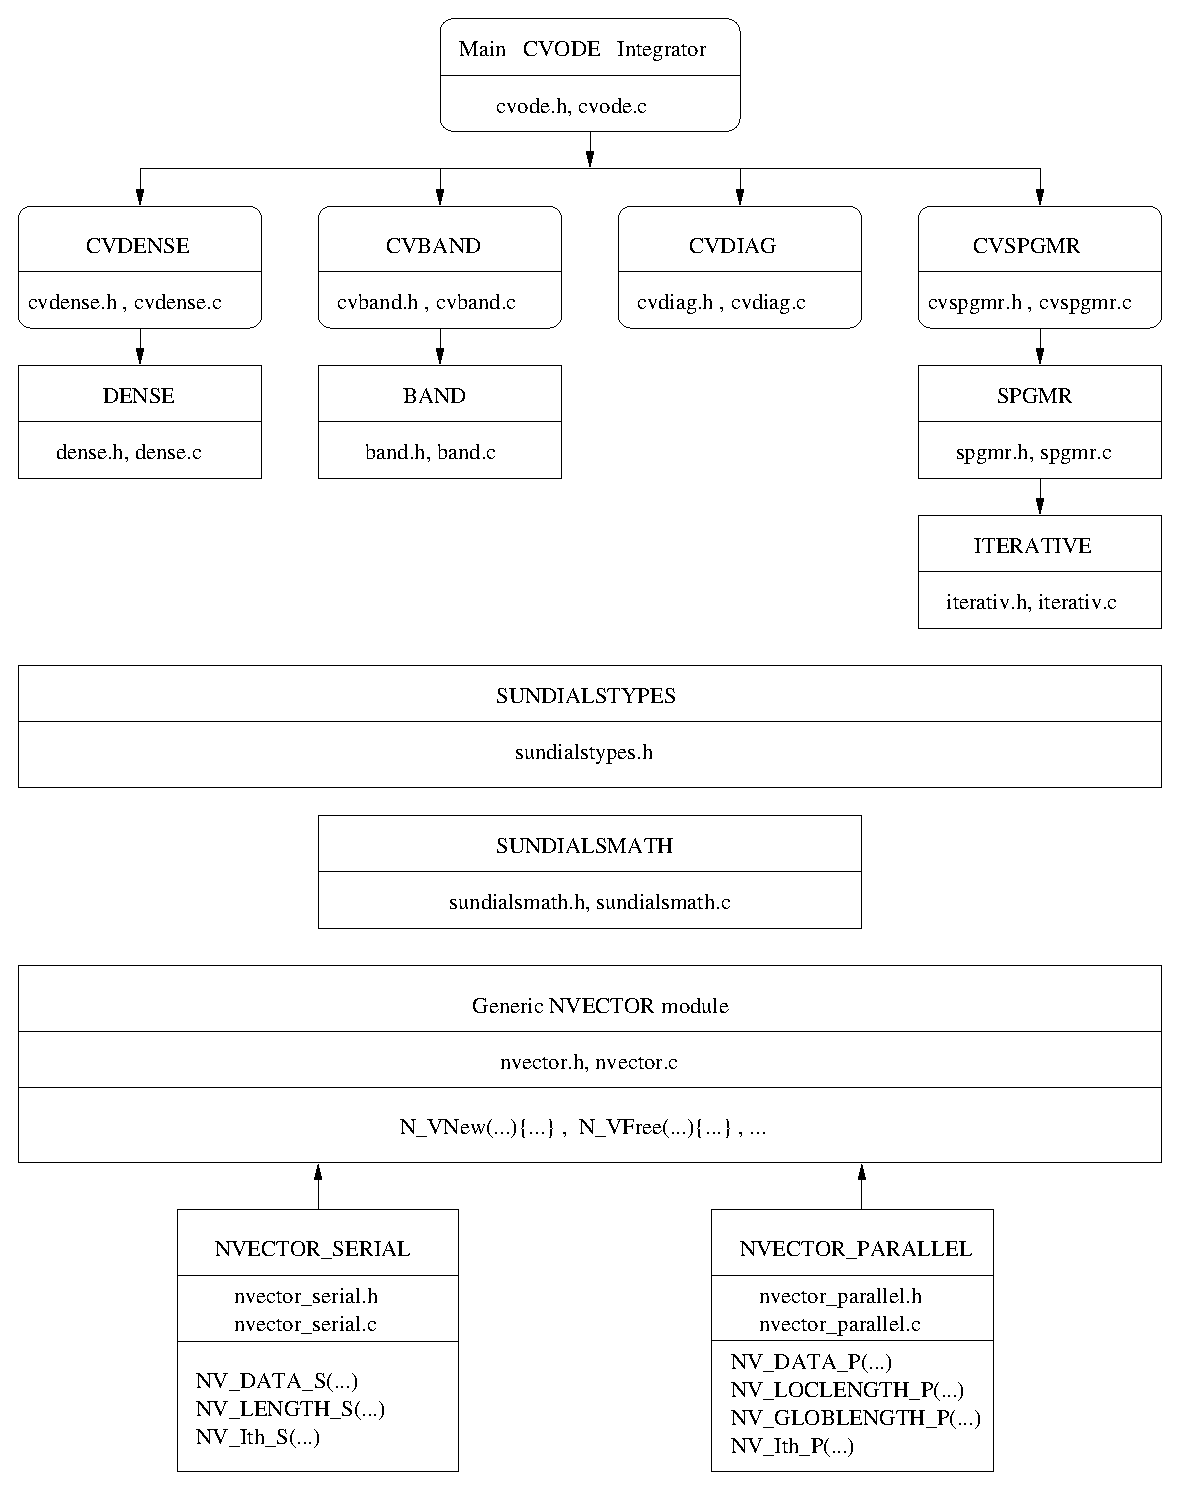
\includegraphics[width=\textwidth]{cvorg}}}
\caption [Overall structure diagram of the {\cvode} package]
{Overall structure diagram of the {\cvode} package.
  Modules specific to {\cvode} begin with ``CV'' ({\cvls},  {\cvnls}, {\cvdiag},
  {\cvbbdpre}, and {\cvbandpre}), all other items correspond to generic
  {\sundials} vector, matrix, and solver modules (see Figure \ref{f:sunorg1}).}
\label{f:cvorg}
\end{figure}
The central integration module, implemented in the files \id{cvode.h},
\id{cvode\_impl.h}, and \id{cvode.c}, deals with the evaluation of integration
coefficients, estimation of local
error, selection of stepsize and order, and interpolation to user output
points, among other issues.

{\cvode} utilizes generic linear and nonlinear solver modules defined by the
{\sunlinsol} API (see Chapter \ref{s:sunlinsol}) and {\sunnonlinsol} API (see
Chapter \ref{c:sunnonlinsol}) respectively. As such, {\cvode} has no knowledge
of the method being used to solve the linear and nonlinear systems that
arise. For any given user problem, there exists a single nonlinear solver
interface and, if necessary, one of the linear system solver interfaces is
specified, and invoked as needed during the integration.

\index{CVODE@{\cvode} linear solver interfaces|(}
At present, the package includes two linear solver interfaces.  The
primary linear solver interface, {\cvls}, supports both direct and
iterative linear solvers built using the generic {\sunlinsol} API (see
Chapter \ref{s:sunlinsol}).  These solvers may utilize a {\sunmatrix}
object (see Chapter \ref{s:sunmatrix}) for storing Jacobian
information, or they may be matrix-free. Since {\cvode} can operate on
any valid {\sunlinsol} implementation, the set of linear solver
modules available to {\cvode} will expand as new {\sunlinsol} modules
are developed.

Additionally, {\cvode} includes the {\em diagonal} linear solver
interface, {\cvdiag}, that creates an internally generated diagonal
approximation to the Jacobian.
\index{CVODE@{\cvode} linear solver interfaces|)}

For users employing dense or banded Jacobian matrices, {\cvode}
includes algorithms for their approximation through difference
quotients, although the user also has the option of supplying a
routine to compute the Jacobian (or an approximation to it) directly.
This user-supplied routine is required when using sparse or
user-supplied Jacobian matrices.

For users employing matrix-free iterative linear solvers,
\index{Jacobian-vector product!setup and solve phases} {\cvode}
includes an algorithm for the approximation by difference quotients of
the product $Mv$. Again, the user has the option of providing routines
for this operation, in two phases: setup (preprocessing of Jacobian
data) and multiplication.

For preconditioned iterative methods, \index{preconditioning!setup and solve phases}
the preconditioning must be supplied by the user, again in two phases:
setup and solve.  While\index{preconditioning!advice on} there is no
default choice of preconditioner analogous to the difference-quotient
approximation in the direct case, the references
\cite{BrHi:89,Byr:92}, together with the example and demonstration
programs included with {\cvode}, offer considerable assistance in
building preconditioners.

\index{CVODE@{\cvode} linear solvers!implementation details|(}
{\cvode}'s linear solver interface consists of four primary phases,
devoted to (1) memory allocation and initialization, (2) setup of the
matrix data involved, (3) solution of the system, and (4) freeing of memory.
The setup and solution phases are separate because the evaluation of
Jacobians and preconditioners is done only periodically during the
integration, and only as required to achieve convergence.
\index{CVODE@{\cvode} linear solvers!implementation details|)}

{\cvode} also provides two preconditioner modules, for use with any of
the Krylov iterative linear solvers. The first one, {\cvbandpre},
is intended to be used with {\nvecs}, {\nvecopenmp} or {\nvecpthreads}
and provides a banded difference-quotient Jacobian-based
preconditioner, with corresponding setup and solve routines.
The second preconditioner module, {\cvbbdpre}, works in conjunction
with {\nvecp} and generates a preconditioner that is a block-diagonal
matrix with each block being a banded matrix.

All state information used by {\cvode} to solve a given problem is saved
in a structure, and a pointer to that structure is returned to the
user.  There is no global data in the {\cvode} package, and so, in this
respect, it is reentrant. State information specific to the linear
solver is saved in a separate structure, a pointer to which resides in
the {\cvode} memory structure. The reentrancy of {\cvode} was motivated
by the anticipated multicomputer extension, but is also essential
in a uniprocessor setting where two or more problems are solved by
intermixed calls to the package from within a single user program.

\clearemptydoublepage
%===============================================================
% Usage
%===================================================================================
\section{Using {\cvode} for IVP Solution}\label{s:simulation}
%===================================================================================

This section is concerned with the use of {\cvode} for the integration of IVPs.
The following subsections treat the header files, the layout of the user's main
program, description of the {\cvode} user-callable routines, and user-supplied functions 
or routines. The listings of the sample programs in \S\ref{s:sim_examples} may also be helpful. 
Those codes are intended to serve as templates and are included in the {\cvode} package.

The user should be aware that not all linear solver modules are compatible 
with all {\nvector} implementations. 
\index{CVODE@{\cvode} linear solvers!NVECTOR@{\nvector} compatibility}
For example, {\nvecp} is not compatible with the direct dense or direct band 
linear solvers since these linear solver modules need to form the system Jacobian.
The following {\cvode} modules can only be used with {\nvecs}:
{\cvdense}, {\cvband}, and {\cvbandpre}. The preconditioner module {\cvbbdpre}
can only be used with {\nvecp}. 

%------------------------
\subsection{Header Files}\label{ss:header_sim}
%------------------------

The calling program must include several header files so that various macros
and data types can be used. The header files that are always required are:
%
\begin{itemize}
\item  \Id{sundialstypes.h}, 
  which defines the types \id{realtype, integertype, booleantype}
  and constants \id{FALSE} and \id{TRUE};
\item  \Id{cvode.h}, 
  the header file for {\cvode}, which defines the several
  types and various constants, and includes function prototypes.
\end{itemize}
%
The calling program must also include an {\nvector} implementation header file
(see \S\ref{s:nvector} for details).
For the two {\nvector} implementations that are included in the {\cvode} package,
the corresponding header files are:
%
\begin{itemize}
\item \Id{nvector\_serial.h}, 
  which defines the serial implementation {\nvecs};
\item \Id{nvector\_parallel.h}, 
  which defines the parallel MPI implementation, {\nvecp}.
\end{itemize}
%
Note that both these files include in turn the header file \Id{nvector.h} which 
defines the abstract \Id{N\_Vector} and \Id{M\_Env} types. 

Finally, if the user chooses Newton iteration for the solution of the nonlinear systems,
then a linear solver module header file will be required. 
\index{CVODE@{\cvode} linear solvers!header files}
The header files corresponding to the various linear solver options in {\cvode} are:
%
\begin{itemize}
\item \Id{cvdense.h}, 
  which is used with the dense direct linear solver in 
  the context of {\cvode}. This in turn includes a header file (\id{dense.h})
  which defines the \Id{DenseMat} type and corresponding accessor macros; 
\item \Id{cvband.h}, 
  which is used with the band direct linear solver in the
  context of {\cvode}. This in turn includes a header file (\id{band.h})
  which defines the \Id{BandMat} type and corrsponding accessor macros;
\item \Id{cvdiag.h}, which is used with a diagonal linear solver in the
  context of {\cvode};
\item \Id{cvspgmr.h}, 
  which is used with the Krylov solver {\spgmr} in the
  context of {\cvode}. This in turn includes a header file (\id{iterativ.h})
  which enumerates the kind of preconditioning and the choices for the
  Gram-Schmidt process.
\end{itemize}

Other headers may be needed, according as to the choice of
preconditioner, etc. In one of the examples to follow, preconditioning
is done with a block-diagonal matrix. For this, the header
\id{smalldense.h} is included.


%-------------------------------------------------
\subsection{A Skeleton of the User's Main Program}\label{ss:skeleton_sim}
%-------------------------------------------------

A high-level view of the combined user program and {\cvode} package is
shown in Figure~\ref{f:sim_overview}.
\begin{figure}
\centerline{\psfig{figure=cvsim.eps,width=\textwidth}}
\caption {Diagram of the user program and 
  {\cvode} package for integration of IVP}\label{f:sim_overview}
\end{figure}
The following is a skeleton of the user's main program (or calling
program) for the integration of an ODE IVP. Most steps are independent of the {\nvector}
implementation used; where this is not the case, usage specifications are given for the
two implementations provided with {\cvode}: steps marked with {\p} correspond to 
{\nvecp}, while steps marked with {\s} correspond to {\nvecs}.
%
\begin{enumerate}
  
\item {\p}
  \id{MPI\_Init(\&argc, \&argv);} to initialize MPI if used by
  the user's program, aside from the internal use in {\nvecp}.  
  Here \id{argc} and \id{argv} are the command line argument 
  counter and array received by \id{main}.
  
\item Set the problem dimensions:
  \begin{itemize}
  \item {\s}
    Set \id{N}, the problem size $N$.
  \item {\p} 
    Set \id{Nlocal}, the local vector length (the sub-vector
    length for this processor); \id{N}, the global vector length (the
    problem size $N$, and the sum of all the values of \id{Nlocal});
    and the active set of processors.
  \end{itemize}
  
\item Initialize the machine environment variable:
  \begin{itemize}
  \item {\s}
    \id{machEnv = }\Id{M\_EnvInit\_Serial}\id{(N);}
  \item {\p}
    \id{machEnv = }\Id{M\_EnvInit\_Parallel}\id{(comm, Nlocal, N, \&argc, \&argv);}
    Here \id{comm} is the MPI communicator, set in one of two ways: 
    If a proper subset of active processors is to be used, \id{comm} 
    must be set by suitable MPI calls. Otherwise, to specify that all 
    processors are to be used, \id{comm} must be \id{MPI\_COMM\_WORLD}.
  \end{itemize}
  
\item Set the vector \id{y0} of initial values.  Use macros
  defined by a particular {\nvector} implementation:
  \begin{itemize}
  \item {\s} 
    \id{NV\_MAKE\_S(y0, ydata, machEnv);}
  \item {\p} 
    \id{NV\_MAKE\_P(y0, ydata, machEnv);}
  \end{itemize}
  if an existing real array \id{ydata} contains the initial values of $y$.  
  Otherwise, make the call \id{y0 = }\Id{N\_VNew}\id{(machEnv);} and load 
  initial values into the real array defined by:
  \begin{itemize}
  \item {\s}
    \id{NV\_DATA\_S(y0)}
  \item {\p}
    \id{NV\_DATA\_P(y0)}
  \end{itemize}
  
\item\label{i:cvode_malloc} 
  Call \id{cvode\_mem = }\id{CVodeMalloc}\id{(...);} 
  to provide problem specifications,
  allocate internal memory for {\cvode}, 
  provide solution method options and tolerances, and initialize {\cvode}. 
  \id{CVodeMalloc} returns a pointer to the {\cvode} memory structure 
  (for details see \S\ref{sss:cvodemalloc}).
  
\item\label{i:lin_solver} If Newton iteration is chosen, initialize the linear solver module
  with one of the following calls (for details see \S\ref{sss:lin_solv_init}):
  \begin{itemize}
  \item {\s} \id{ier = }\Id{CVDense}\id{(...);}
  \item {\s} \id{ier = }\Id{CVBand}\id{(...);}
  \item \id{ier = }\Id{CVDiag}\id{(...);}
  \item \id{ier = }\Id{CVSpgmr}\id{(...);}
  \end{itemize}
  
\item 
  For each point at which output is desired, call
  \id{ier = }\Id{CVode}\id{(cvode\_mem, tout, y, \&t, itask);}
  Set \id{itask} to \Id{NORMAL} to have the integrator overshoot 
  \id{tout} and interpolate, or \Id{ONE\_STEP} to take a single 
  step and return. The vector \id{y} (which can be the same as
  the vector \id{y0} above) will contain $y(t)$.
  
\item Upon completion of the integration, deallocate memory for the vector \id{y}
  by either calling a macro defined by the {\nvector} implementation:
  \begin{itemize}
  \item {\s} 
    \id{NV\_DISPOSE\_S(y);}
  \item {\p}
    \id{NV\_DISPOSE\_P(y);}
  \end{itemize}
  if \id{y} was created from \id{ydata}, or by making the call 
  \Id{N\_VFree}\id{(y);} if \id{y} was created by a call to \id{N\_VNew}.
  
\item \Id{CVodeFree}\id{(cvode\_mem);} to free the memory allocated for {\cvode}.
  
\item Free the machine environment variable:
  \begin{itemize}
  \item {\s}
    \Id{M\_EnvFree\_Serial}\id{(machEnv);}
  \item {\p}
    \Id{M\_EnvFree\_Parallel}\id{(machEnv);}
  \end{itemize}
  
\end{enumerate}

%-------------------------------------------------------
\subsection{User-Callable Routines for IVP Solution}
\label{ss:cvodes_fct_sim}
%-------------------------------------------------------

\subsubsection{{\cvode} Initialization Routine}\label{sss:cvodemalloc}

The form of the call to \ID{CVodeMalloc} (step \ref{i:cvode_malloc}) is
\begin{verbatim}
cvode_mem = CVodeMalloc(f, t0, y0, lmm, iter, itol, &rtol, 
                        atol, f_data, errfp, optIn, iopt, ropt, machEnv);
\end{verbatim}
\id{f} is the C function to compute $f$ in the ODE, \id{t0} is the initial
value of $t $ and \id{y0} is the initial value of $y$. 
\id{f} has the form \id{f(N, t, y, ydot, f\_data)} (for full details
see \S\ref{ss:user_fct_sim}).
The flag \id{lmm} is used to select the linear multistep method and may be one of two
possible values: \Id{ADAMS} or \Id{BDF}. The type of iteration is
selected by replacing \id{iter} with either \Id{NEWTON} or 
\Id{FUNCTIONAL}. The typical choices for (\id{lmm}, \id{iter}) are
(\id{ADAMS}, \id{FUNCTIONAL}) for nonstiff problems and
(\id{BDF}, \id{NEWTON}) for stiff problems.
The next three parameters are used to set the error control. 
The flag \id{itol} is replaced by either \Id{SS} or 
\Id{SV}, where \id{SS} indicates scalar relative error tolerance and
scalar absolute error tolerance, while \id{SV} indicates scalar
relative error tolerance and vector absolute error tolerance. The
latter choice is important when the absolute error tolerance needs to
be different for each component of the ODE. The arguments \id{\&rtol}
and \id{atol} are pointers to the user's error tolerances, and 
\id{f\_data} is a pointer to user-defined space passed directly to
the user's \id{f} function. The file pointer \id{errfp} points to
the file where error messages from {\cvode} are to be written 
(\id{NULL} for \id{stdout}). 
The final argument, \id{machEnv}, is a pointer to machine 
environment-specific information.

Provision is made for certain optional inputs and optional outputs.
Optional inputs communicated in the \id{CVodeMalloc} call are placed
in the arrays \Id{iopt} and \Id{ropt}.  These include the maximum
order, the tentative initial stepsize, and the maximum stepsize.  Each
{\cvode} linear solver may or may not have optional inputs, which are
passed through the associated initialization call list.  Of the existing four
linear solvers, only {\cvspgmr} has optional inputs.  In any case, there
is a default available for every optional input.  Optional outputs
from the central {\cvode} module are also communicated through the
\id{iopt} and \id{ropt} arrays which are passed to \id{CVodeMalloc}.
They include step and function evaluation counts, current stepsize and
order, and workspace lengths.  Optional outputs
specific to each linear solver are loaded into \id{iopt} and
\id{ropt}, following those from the central integrator module.
For full details on the optional inputs and outputs, see
\S\ref{sss:optional_io}.

If \id{optIn} is \id{FALSE}, then {\cvode} assumes that the user is not providing
any optional input, while if it is \id{TRUE} then all optional inputs 
are examined in \id{iopt} and \id{ropt}. 

If there was a failure, the return value of \id{CVodeMalloc} is \id{NULL} and
an error message is printed.

\subsubsection{Linear Solver Specification Routines}\label{sss:lin_solv_init}

As previously explained, Newton iteration requires the solution of
linear systems of the form (\ref{e:Newton}).  There are four {\cvode} linear
solvers currently available for this task: {\cvdense}, {\cvband}, {\cvdiag},
and {\cvspgmr}.  The first three are direct solvers and derive their name
from the type of approximation used for the Jacobian 
$J = \partial{f}/\partial{y}$.  {\cvdense}, {\cvband}, and {\cvdiag} work with
dense, banded, and diagonal approximations to $J$, respectively.  The
fourth {\cvode} linear solver, {\cvspgmr}, is an iterative solver.  The {\spgmr}
in the name indicates that it uses a scaled preconditioned
GMRES method.

\index{CVODE@{\cvode} linear solvers!selecting one|(} 
To specify a {\cvode} linear solver, after the call to \id{CVodeMalloc}
but before any calls to \id{CVode}, the user's program must call one
of the functions \Id{CVDense}, \Id{CVBand}, \Id{CVDiag}, \Id{CVSpgmr},
as documented below. The first argument passed to these functions is the {\cvode}
memory pointer returned by \id{CVodeMalloc}.  A call to one of these
functions links the main {\cvode} integrator to a linear solver and
allows the user to specify parameters which are specific to a
particular solver, such as the bandwidths in the {\cvband} case.

The use of each of the linear solvers involves certain constants (such
as locations of optional outputs in \Id{iopt}), and possibly some
macros, that are likely to be needed in the user code.  These are
available in the corresponding header file associated with the linear
solver, as specified below.
\index{CVODE@{\cvode} linear solvers!selecting one|)}

\index{CVODE@{\cvode} linear solvers!built on generic solvers|(} 
In each case except the diagonal approximation case {\cvdiag}, the linear
solver module used by {\cvode} is actually built on top of a generic
linear system solver, which may be of interest in itself.  These
generic solvers, denoted {\dense}, {\band}, and {\spgmr}, are described
separately in \S\ref{s:gen_linsolv}.
\index{CVODE@{\cvode} linear solvers!built on generic solvers|)}
%
\begin{itemize}
%
%--------------------------------
%
\item {\em Dense linear solver specification} 
  \index{CVODE@{\cvode} linear solvers!CVDENSE@{\cvdense}}

  \index{CVDENSE@{\cvdense} linear solver!selection of|(}
  In using the {\cvdense} solver with {\cvode}, the calling program must
  include the corresponding header file, with the line
\begin{verbatim}
#include "cvdense.h"
\end{verbatim}
  \par After the call to \id{CVodeMalloc}, the user must call the routine \ID{CVDense}
  to select the {\cvdense} solver. The call to this routine has the following form:
\begin{verbatim}
ier = CVDense(cvode_mem, N, djac, jac_data);
\end{verbatim}
  \index{CVDENSE@{\cvdense} linear solver!selection of|)}

  \index{CVDENSE@{\cvdense} linear solver!NVECTOR@{\nvector} compatibility}
  Note that the {\cvdense} linear solver may not be compatible with a particular
  implementation of the {\nvector} module. Of the two {\nvector} modules 
  provided by {\sundials}, only {\nvecs} is compatible, while {\nvecp} is not.

  The \index{CVDENSE@{\cvdense} linear solver!Jacobian approximation used by}
  {\cvdense} solver needs a routine to compute a dense approximation to
  the Jacobian matrix $J(t,y)$.  This routine must be of type
  \id{CVDenseJacFn}, and is communicated through the \id{CVDense} 
  formal parameter \id{djac} (see \S\ref{ss:user_fct_sim} for specification
  details).  The user can supply his/her own dense
  Jacobian routine, or use the difference quotient routine \Id{CVDenseDQJac} 
  \index{Jacobian approximation routine!dense!difference quotient}
  that comes with the {\cvdense} solver.  To use \id{CVDenseDQJac}, the user 
  must pass \id{NULL} for the \id{djac} parameter.
  
  The\index{Jacobian approximation routine!dense!user-supplied}
  \id{CVDense} formal parameter \id{jac\_data} is a pointer that
  accommodates a user-defined data structure. The {\cvdense} solver
  passes the pointer it receives in the \id{CVDense} call to its dense
  Jacobian function (the \id{djac} parameter). This allows the user to
  create an arbitrary structure with relevant problem data and access it
  during the execution of the user-supplied Jacobian routine, without
  using global data in the program.  The pointer \id{jac\_data} may be
  identical to \id{f\_data}, if the latter is passed to
  \id{CVodeMalloc}.
  
  The return value \id{ier} of \id{CVDense} is
  \begin{itemize}
  \item \id{SUCCESS}
    if the {\cvdense} initialization was successful;
  \item \id{LMEM\_FAIL}
    if \id{cvode\_mem} was \id{NULL}, if the {\nvector} module is incompatible 
    with {\cvdense}, or if there was a memory allocation failure.
  \end{itemize}
  
  The {\cvdense} module provides three optional outputs.
  \index{CVDENSE@{\cvdense} linear solver!optional outputs}
  One is the number of calls made to the Jacobian routine. It is placed
  in \id{iopt[}\Id{DENSE\_NJE}\id{]}, where \id{iopt} is the array supplied by the
  user in the \id{CVodeMalloc} call.  The other two are the sizes of the
  real and integer workspaces used by {\cvdense}, stored in
  \id{iopt[}\Id{DENSE\_LRW}\id{]} and \id{iopt[}\Id{DENSE\_LIW}\id{]},
  respectively.
  In \index{CVDENSE@{\cvdense} linear solver!memory requirements} 
  terms of the problem size $N$, the actual sizes of these workspaces are 
  $2N^2$ realtype words and $N$ integertype words.
%
%--------------------------------
%
\item {\em Banded linear solver specification}
  \index{CVODE@{\cvode} linear solvers!CVBAND@{\cvband}}
  
  \index{CVBAND@{\cvband} linear solver!selection of|(}
  In using the {\cvband} solver with {\cvode}, the calling program must
  include the corresponding header file, with the line
\begin{verbatim}
#include "cvband.h"
\end{verbatim}
  \par After the call to \id{CVodeMalloc}, the user must call the routine \ID{CVBand}
  to select the {\cvband} solver. The call to this routine has the following form:
\begin{verbatim}
ier = CVBand(cvode_mem, N, mupper, mlower, bjac, jac_data);
\end{verbatim}
  The upper and lower half-bandwidths of problem Jacobian (or of the
  approximation of it to be used in {\cvode}) are specified in this call
  through the \id{mupper} and \id{mlower} parameters.
  \index{CVBAND@{\cvband} linear solver!selection of|)}
  
  \index{CVBAND@{\cvband} linear solver!NVECTOR@{\nvector} compatibility}
  Note that the {\cvband} linear solver may not be compatible with a particular
  implementation of the {\nvector} module. Of the two {\nvector} modules 
  provided by {\sundials}, only {\nvecs} is compatible, while {\nvecp} is not.

  The \index{CVBAND@{\cvband} linear solver!Jacobian approximation used by} 
  {\cvband} solver requires a routine to compute a banded approximation
  to the Jacobian matrix $J(t,y)$.  This routine must be of type
  \id{CVBandJacFn}, and is communicated through the \id{CVBand} formal 
  parameter \id{bjac} (see \S\ref{ss:user_fct_sim} for specification details).  
  The user can supply his/her own banded Jacobian 
  approximation routine, or use the difference quotient routine 
  \Id{CVBandDQJac} \index{Jacobian approximation routine!band!difference quotient}
  that comes with the {\cvband} solver.  To use the \id{CVBandDQJac}, the user 
  must pass \id{NULL} for \id{bjac}.
  
  As\index{Jacobian approximation routine!band!user-supplied}
  in the {\cvdense} case, the \id{CVBand} formal parameter
  \id{jac\_data} is a pointer to a user-defined data structure, which
  the {\cvband} solver passes to the Jacobian function \id{bjac}.  This
  allows the user to create an arbitrary structure with relevant problem
  data and access it during the execution of the user-supplied Jacobian
  routine, without using global data in the program.  The pointer
  \id{jac\_data} may be identical to \id{f\_data}, if the latter is
  passed to \id{CVodeMalloc}.
  
  The return value \id{ier} of \id{CVBand} is
  \begin{itemize}
  \item \id{SUCCESS}
    if the {\cvband} initialization was successful;
  \item \id{LMEM\_FAIL}:
    if \id{cvode\_mem} was \id{NULL}, if the {\nvector} module is incompatible 
    with {\cvband}, or if there was a memory allocation failure;
  \item \id{LIN\_ILL\_INPUT}
    if there was an illegal input.
  \end{itemize}
  
  The {\cvband} module provides three optional outputs.
  \index{CVBAND@{\cvband} linear solver!optional outputs}
  One is the number of calls made to the Jacobian routine. It is placed
  in \id{iopt[}\Id{BAND\_NJE}\id{]}, where \id{iopt} is the array supplied by the
  user in the \id{CVodeMalloc} call.  The other two are the sizes of the
  real and integer workspaces used by {\cvband}, stored in
  \id{iopt[}\Id{BAND\_LRW}\id{]} and \id{iopt[}\Id{BAND\_LIW}\id{]},
  respectively.
  In \index{CVBAND@{\cvband} linear solver!memory requirements} terms of the problem
  size $N$, the actual sizes of these workspaces are (roughly)
  $N*($2 \id{mupper} + 3 \id{mlower} + 2) realtype words and $N$ integertype
  words.
%
%--------------------------------
%
\item {\em Diagonal linear solver specification}
  \index{CVODE@{\cvode} linear solvers!CVDIAG@{\cvdiag}}
  
  \index{CVDIAG@{\cvdiag} linear solver!selection of|(}
  In using the {\cvdiag} solver with {\cvode}, the calling program must
  include the corresponding header file, with the line
\begin{verbatim}
#include "cvdiag.h"
\end{verbatim}
  \par After the call to \id{CVodeMalloc}, the user must call the routine \ID{CVDiag}
  to select the {\cvdiag} solver. The call to this routine has the following form:
\begin{verbatim}
ier = CVDiag(cvode_mem);
\end{verbatim}
  \index{CVDIAG@{\cvdiag} linear solver!selection of|)}
  
  The {\cvdiag} solver is the simplest of all the current {\cvode} linear
  solvers.  The \id{CVDiag} routine receives only the {\cvode} memory
  pointer returned by \id{CVodeMalloc}.
  The \index{CVDIAG@{\cvdiag} linear solver!Jacobian approximation used by}
  {\cvdiag} solver uses an approximate diagonal Jacobian formed by way of a difference quotient.
  The user does {\em not} have the option to supply a routine to compute
  an approximate diagonal Jacobian.
  
  The return value \id{ier} of \id{CVDiag} is
  \begin{itemize}
  \item \id{SUCCESS}
    if the {\cvdiag} initialization was successful;
  \item \id{LMEM\_FAIL}
    if \id{cvode\_mem} was \id{NULL}, or if there was a memory allocation failure.
  \end{itemize}
  
  The {\cvdiag} module provides two optional outputs.
  \index{CVDIAG@{\cvdiag} linear solver!optional outputs} 
  These are the sizes of the real and integer workspaces used by {\cvdiag}, stored in
  \id{iopt[}\Id{DIAG\_LRW}\id{]} and \id{iopt[}\Id{DIAG\_LIW}\id{]},
  respectively.
  In\index{CVDIAG@{\cvdiag} linear solver!memory requirements} terms of the
  problem size $N$, the actual sizes of these workspaces are
  $3N$ realtype words and no integertype words. The number of approximate
  diagonal Jacobians formed is equal to \id{iopt[NSETUPS]}.
%
%--------------------------------
%
\item {\em {\spgmr} linear solver specification}
  \index{CVODE@{\cvode} linear solvers!CVSPGMR@{\cvspgmr}}
  
  The {\cvspgmr} solver uses a scaled preconditioned GMRES iterative method
  to solve the linear system (\ref{e:Newton}).
  
  \index{preconditioning!advice on|(} 
  With this {\spgmr} method, preconditioning can be done on the left only,
  on the right only, on both the left and the right, or not at all.  For
  a given preconditioner matrix, the merits of left vs. right
  preconditioning are unclear in general, and the user should experiment
  with both choices.  Performance will differ because the inverse of the
  left preconditioner is included in the linear system residual whose
  norm is being tested in the {\spgmr} algorithm.  As a rule, however, if
  the preconditioner is the product of two matrices, we recommend that
  preconditioning be done either on the left only or the right only,
  rather than using one factor on each side.
  \index{preconditioning!advice on|)}
  
  \index{CVSPGMR@{\cvspgmr} linear solver!selection of|(} 
  In using the {\cvspgmr} solver with {\cvode}, the calling program must
  include two associated header files, with the lines
\begin{verbatim}
#include "iterativ.h"
#include "cvspgmr.h"
\end{verbatim}
  \par After the call to \id{CVodeMalloc}, the user must call the routine \ID{CVSpgmr}
  to select the {\cvdiag} solver. This routine has the following form:
\begin{verbatim}
ier = CVSpgmr(cvode_mem, pretype, gstype, maxl, delt, Precond, 
              PSolve, P_data, jtimes, jac_data);
\end{verbatim}
  \index{CVSPGMR@{\cvspgmr} linear solver!selection of|)}
  
  The call to \id{CVSpgmr} is used to communicate the type of
  preconditioning (\id{pretype}), the user's preconditioner setup
  routine (\id{precond}), the preconditioner solve routine (\id{psolve}),
  and the type of Gram-Schmidt procedure (\id{gstype}). The \id{pretype}
  parameter can be \id{NONE}, \id{LEFT}, \id{RIGHT}, or \id{BOTH}.
  (These constants are defined in \id{iterativ.h}.)  If no preconditioning
  is desired (pass \id{NONE} for \id{pretype}), then both \id{precond} and
  \id{psolve} are ignored.  Otherwise, a preconditioner solve function
  \id{psolve} is required.  Regardless of the type of preconditioning,
  a preconditioner setup function \id{precond} is {\em not} required. 
  The \id{gstype} parameter can be \id{MODIFIED\_GS} or \id{CLASSICAL\_GS}
  (these constants are also defined in \id{iterativ.h}) according to
  whether the user wants the {\cvspgmr} solver to use modified or classical
  Gram-Schmidt\index{Gram-Schmidt procedure} orthogonalization.
  
  \index{CVSPGMR@{\cvspgmr} linear solver!optional inputs|(}
  The call to \id{CVSpgmr} is also used to communicate two optional
  inputs to the {\cvspgmr} solver.  One is \id{maxl}, the maximum dimension
  of the Krylov subspace to be used.  The other is \id{delt}, a factor
  by which the GMRES\index{GMRES method} convergence test constant is reduced
  from the Newton iteration test constant.  Both of these inputs have defaults,
  which can be invoked by setting the actual parameter to zero in the
  call.  The actual default values are $5$ for the maximum Krylov
  dimension, and $.05$ for the test constant factor.
  \index{CVSPGMR@{\cvspgmr} linear solver!optional inputs|)}
  
  The routine \id{CVSpgmr} takes in a parameter
  \id{P\_data}, a pointer to a user-defined data structure, which
  the {\cvspgmr} solver passes to the preconditioner setup and solve
  functions \id{precond} and \id{psolve}.  This allows the user to
  create an arbitrary structure with relevant problem data and access it
  during the execution of the user-supplied preconditioner routines
  without using global data in the program.  The pointer \id{P\_data}
  may be identical to \id{f\_data}, if the latter is passed to
  \id{CVodeMalloc}.
  
  If any type of preconditioning is to be done within the {\spgmr} method,
  then the user must supply a preconditioner solve routine \id{psolve}
  \index{CVSPGMR@{\cvspgmr} linear solver!preconditioner solve routine}
  (see \S\ref{ss:user_fct_sim}).
  The evaluation and preprocessing of any Jacobian-related data needed
  by the user's preconditioner solve routine is done in the optional
  user-supplied routine \id{precond}
  \index{CVSPGMR@{\cvspgmr} linear solver!preconditioner setup routine}
  (see \S\ref{ss:user_fct_sim}).
  
  The \index{CVSPGMR@{\cvspgmr} linear solver!Jacobian approximation used by}
  {\cvspgmr} solver requires a routine to compute an approximation to the
  product between the Jacobian matrix $J(t,y)$ and a vector $v$.
  This routine must be of type \id{CVSpgmrJtimesFn}, and is communicated through
  the \id{CVSpgmr} formal parameter \id{jtimes} (see \S\ref{ss:user_fct_sim} for
  specification details).
  The user can supply his/her own Jacobian times vector approximation routine, 
  or use the difference quotient routine \Id{CVSpgmrDQJtimes} 
  \index{Jacobian approximation routine!Jacobian times vector!difference quotient}
  that comes with the {\cvspgmr} solver.  To use the \id{CVSpgmrDQJtimes}, the user 
  must pass \id{NULL} for \id{jtimes}.
  
  As\index{Jacobian approximation routine!Jacobian times vector!user-supplied}
  in the {\cvdense} and {\cvband} cases,  the \id{CVSpgmr} formal parameter
  \id{jac\_data} is a pointer to a user-defined data structure, which
  the {\cvspgmr} solver passes to the Jacobian times vector function \id{jtimes}.  
  This allows the user to create an arbitrary structure with relevant problem
  data and access it during the execution of the user-supplied Jacobian times
  vector routine, without using global data in the program.  The pointer
  \id{jac\_data} may be identical to \id{f\_data}, if the latter is
  passed to \id{CVodeMalloc}.
  
  The return value \id{ier} of \id{CVSpgmr} is
  \begin{itemize}
  \item \id{SUCCESS}
    if the {\cvspgmr} initialization was successful;
  \item \id{LMEM\_FAIL}
    if \id{cvode\_mem} was \id{NULL}, or if there was a memory allocation failure;
  \item \id{LIN\_ILL\_INPUT}
    if there was an illegal input.
  \end{itemize}
  
  The {\cvspgmr} solver provides six optional outputs.
  \index{CVSPGMR@{\cvspgmr} linear solver!optional outputs|(} 
  The total number of calls to \id{precond} is given in \id{iopt[}\Id{SPGMR\_NPE}\id{]},
  and the number of calls to \id{psolve} is in \id{iopt[}\Id{SPGMR\_NPS}\id{]}.
  The number of linear iterations is in \id{iopt[}\Id{SPGMR\_NLI}\id{]},
  and the number of linear convergence failures is in \id{iopt[}\Id{SPGMR\_NCFL}\id{]}.
  The sizes of the real and integer workspaces used by {\cvspgmr} are stored in
  \id{iopt[}\Id{SPGMR\_LRW}\id{]} and \id{iopt[}\Id{SPGMR\_LIW}\id{]}, respectively.
  \index{CVSPGMR@{\cvspgmr} linear solver!optional outputs|)}
  In\index{CVSPGMR@{\cvspgmr} linear solver!memory requirements} terms of the
  problem size $N$ and the maximum Krylov dimension $\ell_{max}$,
  the actual sizes of these workspaces are 
  $N*(\ell_{max} + 5) + \ell_{max}*(\ell_{max} + 4) + 1$ realtype words and
  no integertype words.
  
  \index{SPGMR@{\spgmr} generic linear solver!functions|(}
  For users interested in the generic {\spgmr} solver used by {\cvspgmr}, 
  a note of caution is in order: the routines in {\spgmr} have arguments
  \id{l\_max}, \id{delta}, \id{psolve}, \id{P\_data}, which are {\em not} 
  the same as the \id{CVSpgmr} arguments \id{maxl}, \id{delt}, \id{psolve}, 
  \id{P\_data}, although the names are the same or very similar.
  The arguments \id{pretype} and \id{gstype} are identical in meaning in both
  contexts. For more on the generic {\spgmr} solver, see \S\ref{ss:spgmr}.
  \index{SPGMR@{\spgmr} generic linear solver!functions|)}
  

\end{itemize}


%--------------------------------------------------------------------
\subsubsection{{\cvode} Solver Routine}\label{sss:cvode}

The call to the \ID{CVode} function itself has the form
\begin{verbatim}
ier = CVode(cvode_mem, tout, y, &t, itask);
\end{verbatim}
In addition to the {\cvode} memory pointer \id{cvode\_mem}, it specifies only two
inputs: (1) a flag \id{itask} showing whether the integration is to be done in
the ``normal mode'' or in the ``one-step mode'' and (2) a value,
\id{tout}, of the independent variable $t$ at which a computed
solution is desired.  In the normal mode, the integration proceeds in
steps (with stepsizes determined internally) up to and past \id{tout},
and \id{CVode} interpolates $y$ at $t = $\id{tout}. In the one-step
mode, \id{CVode} takes only one step in the desired direction and
returns to the calling program.  In the one-step mode, \id{tout} is
required on the first call only, to get the direction and rough scale
of the independent variable.  On return, \id{CVode} returns a vector
\id{y} and a corresponding independent variable value
$t=$\id{*t}, such that \id{y} is the computed value of $y(t)$.
In the normal mode, with no failures, \id{*t} will be equal to
\id{tout}.

Note that the vector \id{y} can be the same as the \id{y0} vector of 
initial conditions that was passed to \id{CVodeMalloc}. 

The return value \id{ier} for \id{CVode} will be one of the following:
\begin{itemize}
\item \Id{SUCCESS}=0:
  \id{CVode} succeeded;
\item \Id{TSTOP\_RETURN}=1:
  \id{CVode} succeeded by reaching the stopping point specified through
  the optional inputs \id{iopt[ISTOP]} and \id{ropt[TSTOP]} 
  (see \S\ref{sss:optional_io});
\item \Id{CVODE\_NO\_MEM}:
  The \id{cvode\_mem} argument was \id{NULL};
\item \Id{ILL\_INPUT}:
  One of the inputs to CVode is illegal. This includes the situation when a 
  component of the error weight vectors becomes negative during internal 
  time-stepping. The \id{ILL\_INPUT} flag will also be returned if the linear 
  solver routine initialization (called by the user after calling 
  \id{CVodeMalloc}) failed to set one of the linear solver-related fields 
  in \id{cvode\_mem} or if the linear solver's initialization routine failed. 
  In any case, the user should see the printed error message for more details;
\item \Id{TOO\_MUCH\_WORK}: 
  The solver took mxstep internal steps but could not reach tout. 
  The default value for mxstep is \id{MXSTEP\_DEFAULT = 500};      
\item \Id{TOO\_MUCH\_ACC}: 
  The solver could not satisfy the accuracy demanded by the user for some 
  internal step;
\item \Id{ERR\_FAILURE}: 
  Error test failures occurred too many times (\id{MXNEF = 7}) during one 
  internal time step or occurred with $|h| = h_{min}$;
\item \Id{CONV\_FAILURE}: 
  Convergence test failures occurred too many times (\id{MXNCF = 10}) during 
  one internal time step or occurred with $|h| = h_{min}$;             
\item \Id{SETUP\_FAILURE}: 
  The linear solver's setup routine failed in an unrecoverable manner;
\item \Id{SOLVE\_FAILURE}: 
  The linear solver's solve routine failed in an unrecoverable manner.
\end{itemize} 
All failure return values are negative and therefore a test \id{ier < 0}
will trap all \id{CVode} failures.


%--------------------------------------------------------------------
\subsubsection{Optional Input/Output}\label{sss:optional_io}

In order to change some of the {\cvode} constants (such as the maximum method order) 
or if additional diagnostic output values are desired, tthe user should declare two 
arrays for optional input and output, an \ID{iopt} array for optional integer 
input and output and an \ID{ropt} array for optional real input and output. 
The size of both these arrays should be \id{OPT\_SIZE}.
So the user's declarations should look like:
\begin{verbatim}
long int iopt[OPT_SIZE];
realtype     ropt[OPT_SIZE];
\end{verbatim}
Tables \ref{t:iopt} and \ref{t:ropt} contain 
detailed descriptions of the optional integer and real input-output arrays,
respectively. Only locations corresponding to the main {\cvode} solver are 
given in these tables. Locations beyond \id{CVODE\_IOPT\_SIZE} and
\id{CVODE\_ROPT\_SIZE} in \id{iopt} and \id{ropt}, respectively, are used
by the linear solvers and are described in \S\ref{sss:lin_solv_init}.

Default values of the optional inputs are obtained by setting the corresponding
entry to 0. If \id{FALSE} is passed for \id{optIn} in the call to \id{CVodeMalloc},
no optional input is examined.
%
\begin{table}
\centering
\caption{Description of the optional integer input-output array \Id{iopt}}\label{t:iopt}
\medskip
\begin{tabular}{|l|c|p{1in}|p{3in}|}
\hline
{\bf Index} & {\bf I/O} & {\bf Default value} & {\bf Description} \\ 
\hline\hline
%
\id{MAXORD} & I & 12 (\Id{ADAMS}) & 
Maximum \id{lmm} order to be used by the solver. \\
            &   & 5 (\Id{BDF}) &
\\ \hline
%
\id{MXSTEP} & I & 500 & 
Maximum number of internal steps to be taken by 
the solver in its attempt to reach tout.
\\ \hline
%
\id{MXHNIL} & I & 10 &
Maximum number of warning messages issued by the solver 
that $t+h==t$ on the next internal step. 
A value of -1 means no such messages are issued.
\\ \hline                                                    
%
\id{SLDET} & I & 0 & 
Flag to turn on/off stability limit detection  
(1 = on, 0 = off). When \Id{BDF} is used and order  
is 3 or greater, \id{CVsldet} is called to detect     
stability limit.  If limit is detected, the    
order is reduced.
\\ \hline                                                                 
%
\id{NST} & O & &
Cumulative number of internal steps taken by    
the solver (total so far).
\\ \hline
%                                                                
\id{NFE} & O & &
Number of calls to the user's \id{f} function.
\\ \hline
%
\id{NSETUPS} & O & &
Number of calls made to the linear solver's setup routine.
\\ \hline
%
\id{NNI} & O & &
Number of nonlinear (\Id{FUNCTIONAL} or \Id{NEWTON} iterations performed.         
\\ \hline
%
\id{NCFN} & O & &
Number of nonlinear convergence failures that have occurred.
\\ \hline
%
\id{NETF} & O & &
Number of local error test failures that have occurred.
\\ \hline
%
\id{QU} & O & &
Order used during the last internal step.      
\\ \hline
%
\id{QCUR} & O & &
Order to be used on the next internal step.    
\\ \hline
%
\id{LENRW} & O & &
Size of required {\cvode} internal real work      
space, in realtype words.
\\ \hline
%
\id{LENIW} & O && 
Size of required {\cvode} internal integer work   
space, in integertype words.
\\ \hline                                                                 
%
\id{NOR} & O && 
Number of order reductions due to stability limit detection.
%
\\ \hline

\end{tabular}
\end{table}

\begin{table}
\centering
\caption{Description of the optional real input-output array \Id{ropt}}\label{t:ropt}
\medskip
\begin{tabular}{|l|c|p{1in}|p{3in}|}
\hline
{\bf Index} & {\bf I/O} & {\bf Default value} & {\bf Description} \\ 
\hline\hline
%
\id{H0} & I & computed &
Initial step size.
\\ \hline
%
\id{HMAX} & I & $\infty$ & 
Maximum absolute value of step size allowed.   
Note: If \id{optIn=TRUE}, the value of \id{ropt[HMAX]} 
is examined on every call to \id{CVode}, and so can 
be changed between calls.
\\ \hline
%        
\id{HMIN}    & I & 0.0 & 
Minimum absolute value of step size allowed.   
\\ \hline
%                                                        
\id{HU} & O && 
Step size for the last internal step.          
\\ \hline
%
\id{HCUR} & O && 
Step size to be attempted on the next internal step.
\\ \hline
%
\id{TCUR} & O && 
Current internal time reached by the solver.   
\\ \hline
%
\id{TOLSF} & O && 
A suggested factor by which the user's tolerances 
should be scaled when too much accuracy has been 
requested for some internal step.
\\ \hline
%
\end{tabular}
\end{table}                                                                  

%--------------------------------------------------------------------
\subsubsection{Interpolated Output Routine}
\index{interpolated output}

An optionally callable function \ID{CVodeDky} is available
to obtain additional output values.  This function must be called after a successful
return from \id{CVode} and provides interpolated values of $y$ or its derivatives, 
up to the current order of the integration method, interpolated to any value of $t$ 
in the last internal step taken by {\cvode}.

The call to the \id{CVodeDky} function has the form
\begin{verbatim}
ier = CVodeDky(cvode_mem, t, k, dky);
\end{verbatim}
and computes the \id{k}-th derivative of the \id{y} function at      
time \id{t}, i.e. $d^{(k)}y/dt^{(k)} (t)$, where $t_n - h_u \le$ \id{t} $\le t_n$, 
$t_n$ denotes the current internal time reached, and $h_u$ is the 
last internal step size successfully used by the solver. 
The user may request \id{k} $= 0, 1, ..., q_u$, where $q_u$ is the 
current order. The derivative vector is returned in \id{dky}. 
This vector must be allocated by the caller. 
The first argument \id{cvode\_mem} is the pointer to the {\cvode}
memory returned by \id{CVodeMalloc}.

Note that it is only legal to call the function \id{CVodeDky} after a 
successful return from \id{CVode}.
The return value \id{ier} for \id{CVodeDky} is
\begin{itemize}
\item \Id{OKAY} if \id{CVodeDky} succeeded;
\item \Id{BAD\_K} if \id{k} is not in the range $0, 1, ..., q_u$;
\item \Id{BAD\_T} if \id{t} is not in the interval $[t_n - h_u , t_n]$;
\item \Id{BAD\_DKY} if the \id{dky} argument was \id{NULL};
\item \Id{DKY\_NO\_MEM} if the \id{cvode\_mem} argument was \id{NULL}.
\end{itemize}

%--------------------------------------------------------------------
\subsubsection{{\cvode} Reinitialization Routine}\label{sss:cvreinit}
\index{reinitialization}

The function \ID{CVodeReInit} reinitializes the main {\cvode} solver for
the solution of a problem, where a prior call to \Id{CVodeMalloc} has
been made with the same problem size \id{N}. \id{CVodeReInit} performs the 
same input checking and initializations that \id{CVodeMalloc} does 
(except for \id{N}), but does no memory allocation, assuming that the 
existing internal memory is sufficient for the new problem.             
                                                                 
The use of \id{CVodeReInit} requires that the maximum method order,    
\Id{maxord}, is no larger for the new problem than for the problem  
specified in the last call to \id{CVodeMalloc}.  This condition is  
automatically fulfilled if the multistep method parameter \id{lmm}  
is unchanged (or changed from \Id{ADAMS} to \Id{BDF}) and the default    
value for \id{maxord} is specified.                                 
                                                                 
If \id{iter = }\Id{NEWTON}, then following the call to \id{CVodeReInit}, a call  
to the linear solver specification routine is necessary if a   
different linear solver is chosen, but may not be otherwise.   
If the same linear solver is chosen, and there are no changes  
in the input parameters to the specification routine, then no  
call to that routine is needed.                                
If there are changes in parameters, but they do not increase   
the linear solver memory size, then a call to the corresponding
\id{CVReInit<linsol>} routine must made to communicate the new      
parameters (see \S\ref{sss:lin_solv_reinit}); 
in that case the linear solver memory is reused.   
If the parameter changes do increase the linear solver memory  
size, then the main linear solver specification routine must be
called (\S\ref{sss:lin_solv_init}).

The call to the \id{CVodeReInit} function has the form
\begin{verbatim}
ier = CVodeReInit(cvode_mem, f, t0, y0, lmm, iter, itol, &rtol, 
                  atol, f_data, errfp, optIn, iopt, ropt, machEnv);
\end{verbatim}
Its first argument, \id{cvode\_mem} is the pointer to the {\cvode}
memory returned by \id{CVodeMalloc}.
All the remaining arguments to \id{CVodeReInit} have names and         
meanings identical to those of \id{CVodeMalloc}.  Note that the     
problem size \id{N} is not passed as an argument to \id{CVodeReInit},       
as that is assumed to be unchanged since the \id{CVodeMalloc} call. 

The return value \id{ier} of \id{CVodeReInit} is equal to: 
\begin{itemize}
\item \id{SUCCESS}=0 if there were no errors; 
\item \id{CVREI\_NO\_MEM} if \id{cvode\_mem} was NULL;
\item \id{CVREI\_ILL\_INPUT} if an input argument was illegal    
      (including an attempt to increase \id{maxord}).
\end{itemize}
In case of an error return, an error message is also printed.  

Finally, note that the reported workspace sizes \Id{iopt}\id{[LENRW]} 
and \Id{iopt}\id{[LENIW]} are left unchanged from the values computed 
by \id{CVodeMalloc}, and so may be larger than would be computed for 
the new problem.

%--------------------------------------------------------------------
\subsubsection{Linear Solver Reinitialization Routines}\label{sss:lin_solv_reinit}
\index{reinitialization}

\index{CVODE@{\cvode} linear solvers!reinitializing one|(} 
Linear solver reinitialization routines reset the link between the main {\cvode}
integrator and the linear solver module. Such a routine must be called after a call
to \Id{CVodeReInit} to solve another problem of the same size if there is a change
in some of the linear solver parameters (such as the Jacobian data approximation
routine or the user-defined data structure). Reinitialization routines exist for
all but the {\cvdiag} linear solver.

\begin{itemize}

\item {\em Dense linear solver reinitialization} 
  \index{CVODE@{\cvode} linear solvers!CVDENSE@{\cvdense}}

  \index{CVDENSE@{\cvdense} linear solver!reinitialization|(}
  A call to the \ID{CVReInitDense} function resets the link between   
  the main {\cvode} integrator and the {\cvdense} linear solver.       
  After solving one problem using {\cvdense}, call \id{CVodeReInit} and then
  \id{CVReInitDense} to solve another problem of the same size, if    
  there is a change in the \id{CVDense} parameters \id{djac} or \id{jac\_data}.  
  If there is no change in parameters, it is not necessary to    
  call either \id{CVReInitDense} or \id{CVDense} for the new problem.  

  The call to the {\cvdense} reinitialization routine has the following form:
\begin{verbatim}
ier = CVReInitDense(cvode_mem, djac, jac_data);
\end{verbatim}
  All arguments to \id{CVReInitDense} have the same names and meanings
  as those of \id{CVDense}.  The \id{cvode\_mem} argument must be identical 
  to its value in the previous \id{CVDense} call.                     
  
  The return values of \id{CVReInitDense} are:
  \begin{itemize}
  \item \Id{SUCCESS} if successful;
  \item \Id{LMEM\_FAIL} if the \id{cvode\_mem} argument is \id{NULL}.
  \end{itemize}         
  
  Note that \id{CVReInitDense} performs the same tests for a compatible {\nvector} 
  \index{CVDENSE@{\cvdense} linear solver!NVECTOR@{\nvector} compatibility} 
  module as \id{CVDense}.
  \index{CVDENSE@{\cvdense} linear solver!reinitialization|)}
  
\item {\em Banded linear solver reinitialization}
  \index{CVODE@{\cvode} linear solvers!CVBAND@{\cvband}}
  
  \index{CVBAND@{\cvband} linear solver!reinitialization|(}
  A call to the \ID{CVReInitBand} function resets the link between    
  the main {\cvode} integrator and the {\cvband} linear solver.        
  After solving one problem using {\cvband}, call \id{CVodeReInit} and then 
  \id{CVReInitBand} to solve another problem of the same size, if     
  there is a change in the \id{CVBand} parameters \id{bjac} or \id{jac\_data},   
  but no change in \id{mupper} or \id{mlower}.  If there is a change in    
  \id{mupper} or \id{mlower}, then \id{CVBand} must be called again, and the    
  linear solver memory will be reallocated.                      
  If there is no change in parameters, it is not necessary to    
  call either \id{CVReInitBand} or \id{CVBand} for the new problem.

  The call to the {\cvband} reinitialization routine has the following form:
\begin{verbatim}
ier = CVReInitBand(cvode_mem, mupper, mlower, bjac, jac_data);
\end{verbatim}
  All arguments to \id{CVReInitBand} have the same names and meanings
  as those of \id{CVBand}.  The \id{cvode\_mem} argument must be identical 
  to its value in the previous \id{CVBand} call.                     
  
  The return values of \id{CVReInitBand} are:
  \begin{itemize}
  \item \Id{SUCCESS} if successful;
  \item \Id{LMEM\_FAIL} if the \id{cvode\_mem} argument is \id{NULL};
  \item \Id{LIN\_ILL\_INPUT} if there was an illegal input.
  \end{itemize}         
  
  Note that \id{CVReInitBand} performs the same tests for a compatible {\nvector} 
  \index{CVBAND@{\cvband} linear solver!NVECTOR@{\nvector} compatibility} 
  module as \id{CVBand}.  
  \index{CVBAND@{\cvband} linear solver!reinitialization|)}

\item {\em {\spgmr} linear solver reinitialization}
  \index{CVODE@{\cvode} linear solvers!CVSPGMR@{\cvspgmr}}
  
  \index{CVSPGMR@{\cvspgmr} linear solver!reinitialization|(}
  A call to the \ID{CVReInitSpgmr} function resets the link between   
  the main {\cvode} integrator and the {\cvspgmr} linear solver.       
  After solving one problem using {\cvspgmr}, call \id{CVodeReInit} and then
  \id{CVReInitSpgmr} to solve another problem of the same size, if    
  there is a change in the \id{CVSpgmr} parameters \id{pretype}, \id{gstype},   
  \id{delt}, \id{precond}, \id{psolve}, \id{P\_data}, \id{jtimes}, or 
  \id{jac\_data}, but not in \id{maxl}.  
  If there is a change in \id{maxl}, then \id{CVSpgmr} must be      
  called again, and the linear solver memory will be reallocated.
  If there is no change in parameters, it is not necessary to    
  call either \id{CVReInitSpgmr} or \id{CVSpgmr} for the new problem.

  The call to the {\cvspgmr} reinitialization routine has the following form:
\begin{verbatim}
ier = CVReInitSpgmr(cvode_mem, pretype, gstype, maxl, delt, Precond, 
                    PSolve, P_data, jtimes, jac_data);
\end{verbatim}
  All arguments to \id{CVReInitSpgmr} have the same names and meanings
  as those of \id{CVSpgmr}.  The \id{cvode\_mem} argument must be identical 
  to its value in the previous \id{CVSpgmr} call.                     
  
  The return values of \id{CVReInitSpgmr} are:
  \begin{itemize}
  \item \Id{SUCCESS} if successful;
  \item \Id{LMEM\_FAIL} if the \id{cvode\_mem} argument is \id{NULL};
  \item \Id{LIN\_ILL\_INPUT} if there was an illegal input.
  \end{itemize}         
  \index{CVSPGMR@{\cvspgmr} linear solver!reinitialization|)}

\end{itemize}

%--------------------------------------------------------------------
\subsubsection{Additional Extraction Routines}\label{sss:cvodegetewt}
\index{access to additional data}

Users that wish to supply thier own finite-difference based Jacobian routines
(see \S\ref{ss:user_fct_sim}) may find it usefull to have access to the
vector of error weights that is already available in the {\cvode} internal 
memory block. This information can be extracted with a call to the function
\ID{CVodeGetEwt}.
The call to this function has the form
\begin{verbatim}
ier = CVodeGetEwt(cvode_mem, weight);
\end{verbatim}
where \id{cvode\_mem} is the pointer to the {\cvode} memory returned by
\id{CVodeMalloc} and \id{weight} is an {\nvector} wich will contain
the solution error weights at the current time. Note that the user need not
allocate space for \id{weight}.

Additionally, the machine unit roundoff can be obtained by callingwith
the call
\begin{verbatim}
uround = UnitRoundoff();
\end{verbatim}
The function \Id{UnitRoundoff}, defined in \id{sundialsmath} returns a
\id{realtype} value equal to the machine unit roundoff.

                                                                 
%----------------------------------
\subsection{User-Supplied Routines for IVP Solution}\label{ss:user_fct_sim}
%----------------------------------

The user-supplied routines consist of one function defining the ODE, 
(optionally) a function that provides Jacobian related information for the linear 
solver (if Newton iteration is chosen), and (optionally) one or two functions 
that define the preconditioner for use in the {\spgmr} algorithm. 

\begin{itemize}
%
%--------------
%
\item {\em ODE right hand side}
  \index{right hand side function!initial value problem|(}

  The user must provide a function of type \ID{RhsFn} defined by
\begin{verbatim}
typedef void (*RhsFn)(realtype t, N_Vector y, N_Vector ydot, void *f_data);
\end{verbatim}
  to compute the right hand side of the ODE system.
  
  This function takes as input the independent variable  
  value \id{t} and the dependent variable vector \id{y}.  It must store the    
  result of $f(t,y)$ in the vector \id{ydot}.  The \id{y} and \id{ydot} arguments 
  are of type \id{N\_Vector}. Allocation of memory for \id{ydot} is handled within {\cvode}.
  The \id{f\_data} parameter is the same as the \id{f\_data} parameter passed by 
  the user to the \id{CVodeMalloc} routine. This user-supplied pointer is passed to 
  the user's \id{f} function every time it is called.                                       
  A \id{RhsFn} function type does not have a return value.                        
  \index{right hand side function!initial value problem|)}
%
%--------------
%
\item {\em Jacobian information (direct method with dense Jacobian)}
  \label{p:djac}
  \index{Jacobian approximation routine!dense!user-supplied|(}
  
  If the direct linear solver with dense treatment of the Jacobian is used 
  (i.e. \Id{CVDense} is called in step \ref{i:lin_solver} of \S\ref{ss:skeleton_sim}), 
  the user may provide a function of type \ID{CVDenseJacFn} defined by
\begin{verbatim}
typedef void (*CVDenseJacFn)(integertype N, DenseMat J, realtype t, 
                             N_Vector y, N_Vector fy, void *jac_data,
                             N_Vector tmp1, N_Vector tmp2, N_Vector tmp3);
\end{verbatim}
  to compute the dense Jacobian $J = \partial f / \partial y$ (or an approximation to it).
  
  A user-supplied dense Jacobian routine must load the \id{N} by \id{N}
  dense matrix \id{J} with an approximation to the Jacobian matrix $J$
  at the point (\id{t},\id{y}).  Only nonzero elements need to be loaded
  into \id{J} because \id{J} is set to the zero matrix before the call
  to the Jacobian routine. The type of \id{J} is \Id{DenseMat}. The
  accessor macros \Id{DENSE\_ELEM} and \Id{DENSE\_COL} allow the user to
  read and write dense matrix elements without making explicit
  references to the underlying representation of the \id{DenseMat}
  type. \id{DENSE\_ELEM(A,i,j)} references the (\id{i},\id{j})th
  element of the dense matrix \id{A} (\id{i},\id{j} = 0..N-1). This macro
  is for use in small problems in which efficiency of access is not a major
  concern.  Thus, in terms of indices $m$ and $n$ running from $1$ to
  $N$, the Jacobian element $J_{m,n}$ can be loaded with the statement
  \id{DENSE\_ELEM(A,m-1,n-1) =} $J_{m,n}$.  Alternatively,
  \id{DENSE\_COL(A,j)} returns a pointer to the storage for
  the \id{j}th column of \id{A}, and the elements of the \id{j}th column
  are then accessed via ordinary array indexing.  Thus $J_{m,n}$ can be 
  loaded with the statements \id{col\_n = DENSE\_COL(J,n-1);}
  \id{col\_n[m-1] =} $J_{m,n}$.  For large problems, it is more 
  efficient to use \id{DENSE\_COL} than to use \id{DENSE\_ELEM}. 
  Note that both of these macros number rows and columns
  starting from $0$, not $1$.  The \id{DenseMat} type and the accessor
  macros \id{DENSE\_ELEM} and \id{DENSE\_COL} are documented in
  \S\ref{ss:dense}.
  
  The arguments \id{tmp1}, \id{tmp2}, and \id{tmp3} are pointers to 
  memory allocated for vectors of length N which can be used 
  as temporary storage or work space.
  \index{Jacobian approximation routine!dense!user-supplied|)}
%
%--------------
%
\item {\em Jacobian information (direct method with banded Jacobian)}
  \label{p:bjac}
  \index{Jacobian approximation routine!band!user-supplied|(}
  
  If the direct linear solver with banded treatment of the Jacobian is used 
  (i.e. \Id{CVBand} is called in step \ref{i:lin_solver} of \S\ref{ss:skeleton_sim}), 
  the user may provide a function of type \ID{CVBandJacFn} defined by
\begin{verbatim}
typedef void (*CVBandJacFn)(integertype N, integertype mupper, 
                            integertype mlower, BandMat J, realtype t, 
                            N_Vector y, N_Vector fy, void *jac_data,
                            N_Vector tmp1, N_Vector tmp2, N_Vector tmp3);
\end{verbatim}
  to generate the banded Jacobian $J = \partial f / \partial y$ 
  (or a banded approximation to it).
  
  A user-supplied band Jacobian routine must load the band matrix \id{J}
  of type \Id{BandMat} with the elements of the Jacobian $J(t,y)$ at the
  point (\id{t},\id{y}).  Only nonzero elements need to be loaded into
  \id{J} because \id{J} is preset to zero before the call to the
  Jacobian routine.  The accessor macros \Id{BAND\_ELEM},
  \Id{BAND\_COL}, and \Id{BAND\_COL\_ELEM} allow the user to read and 
  write band matrix elements without making specific references to the 
  underlying representation of the \id{BandMat} type.
  \id{BAND\_ELEM(A,i,j)} references the (\id{i},\id{j})th element of the band matrix \id{A}.
  This macro is for use in small problems in which efficiency of access is not
  a major concern.  Thus, in terms of indices $m$ and $n$ running from $1$ to
  $N$ with $(m,n)$ within the band defined by \id{mupper} and
  \id{mlower}, the Jacobian element $J_{m,n}$ can be loaded with the 
  statement \id{BAND\_ELEM(A,m-1,n-1) =} $J_{m,n}$. The elements within
  the band are those with \id{-mupper} $\le$ \id{m-n} $\le$ \id{mlower}.
  Alternatively, \id{BAND\_COL(A,j)} returns a pointer to the diagonal element of the
  \id{j}th column of \id{A}, and if we assign this address to 
  \id{realtype *col\_j}, then the \id{i}th element of the \id{j}th column is
  given by \id{BAND\_COL\_ELEM(col\_j,i,j)}.
  Thus for $(m,n)$ within the band, \\ $J_{m,n}$ can be loaded by setting 
  \id{col\_n = BAND\_COL(J,n-1);} \id{BAND\_COL\_ELEM(col\_n,m-1,n-1) =} $J_{m,n}$.
  The elements of the \id{j}th column can also be accessed
  via ordinary array indexing, but this approach requires knowledge of
  the underlying storage for a band matrix of type \id{BandMat}.  
  The array \id{col\_n} can be indexed from $-$\id{mupper} to \id{mlower}.
  For large problems, it is more efficient to use the combination of
  \id{BAND\_COL} and \id{BAND\_COL\_ELEM} than to use the
  \id{BAND\_ELEM}.  As in the dense case, these macros all number rows
  and columns starting from $0$, not $1$.  The \id{BandMat} type and the
  accessor macros \id{BAND\_ELEM}, \id{BAND\_COL}, and
  \id{BAND\_COL\_ELEM} are documented in \S\ref{ss:band}.
  
  The arguments \id{tmp1}, \id{tmp2}, and \id{tmp3} are pointers to 
  memory allocated for vectors of length N which can be used 
  as temporary storage or work space.
  \index{Jacobian approximation routine!band!user-supplied|)}
%
%----------------
%
\item {\em Jacobian information ({\spgmr} case)}
  \label{p:jtimes}
  \index{Jacobian approximation routine!Jacobian times vector!user-supplied|(}

  If an iterative {\spgmr} linear solver is selected (\id{CVSpgmr} is called in step 
  \ref{i:lin_solver} of \S\ref{ss:skeleton_sim}) the user may provide a function
  of type \ID{CVSpgmrJtimesFn} in the form 
\begin{verbatim}
typedef int (*CVSpgmrJtimesFn)(N_Vector v, N_Vector Jv, realtype t,
                               N_Vector y, N_Vector fy, void *jac_data,
                               N_Vector work);
\end{verbatim} 
  to compute the product $J v = (\partial f / \partial y) v$ (or an approximation to it).
  
  A user-supplied Jacobian-times-vector routine must load the vector \id{Jv}
  with the result of the product between the Jacobian $J(t,y)$ at the
  point (\id{t},\id{y}) and the vector \id{v} of dimension \id{N}.

  The argument \id{work} is a pointer to 
  memory allocated for a vector of length N which can be used 
  as temporary storage or work space.

  The value to be returned by the Jacobian times vector routine should be
  $0$ if successful. Any other return value will result in an unrecoverable
  error of the {\spgmr} generic solver, in which case the integration is halted.
  
  \index{Jacobian approximation routine!Jacobian times vector!user-supplied|)}
%
%--------------
%
\item {\em Preconditioning (linear system solution)}
  \label{p:psolve}
  \index{CVSPGMR@{\cvspgmr} linear solver!preconditioner solve routine}
  
  If preconditioning is used, then the user must provide a {\C} function to
  solve the linear system $Pz = r$ where $P$ may be either a left or a
  right preconditioner matrix.
  This function must be of type \ID{CVSpgmrPSolveFn} defined by
\begin{verbatim}
typedef int (*CVSpgmrPSolveFn)(realtype t, N_Vector y, 
                            N_Vector fy, N_Vector vtemp, realtype gamma, 
                            N_Vector ewt, realtype delta, long int *nfePtr, 
                            N_Vector r, int lr, void *P_data, N_Vector z);
\end{verbatim}
  
  Its parameters are as follows:
  \begin{itemize}
  \item 
    \id{t} is the current value of the independent variable;       
  \item 
    \id{y} is the current value of the dependent variable vector;  
  \item 
    \id{fy} is the vector $f(t,y)$;    
  \item 
    \id{vtemp} is a pointer to memory allocated for a vector of        
    length \id{N} which can be used for work space;    
  \item 
    \id{gamma} is the scalar appearing in the Newton matrix;         
  \item 
    \id{ewt} is the error weight vector (input). See \id{delta} below;   
  \item 
    \id{delta} is an input tolerance to be use if an iterative method 
    is employed in the solution.  In that case, the residual 
    vector $Res = r - P z$ of the system should be made less than 
    \id{delta} in weighted $l_2$ norm,     
    i.e., $\sqrt{\sum_i (Res_i \cdot ewt_i)^2 } < delta$;       
  \item 
    \id{nfePtr} is a pointer to the memory location containing the      
    {\cvode} problem data \id{nfe} = number of calls to \id{f}. 
    The preconditioner solve routine should update this counter by 
    adding on the number of \id{f} calls made in order to carry out     
    the solution, if any.  For example, if the routine      
    calls \id{f} a total of W times, then the update is          
    \id{*nfePtr += W;};         
  \item 
    \id{r} is the right-hand side vector of the linear system;     
  \item 
    \id{lr} is an input flag indicating whether the preconditioner solve
    routine is to use the left preconditioner (\id{lr=1}) or 
    the right preconditioner (\id{lr=2});
  \item 
    \id{P\_data} is a pointer to user data - the same as the \id{P\_data}      
    parameter passed to \id{CVSpgmr};                         
  \item 
    \id{z} is the output vector computed.                
  \end{itemize}
  
  The value to be returned by the preconditioner solve function is a flag indicating 
  whether it was successful.  This value should be $0$ if successful, 
  positive for a recoverable error (in which case the step will be retried),     
  negative for an unrecoverable error (in which case the integration is halted). 
%
%-----------------
%
\item {\em Preconditioning (Jacobian data)}
  \label{p:precond}
  \index{CVSPGMR@{\cvspgmr} linear solver!preconditioner setup routine}
  
  If the user's preconditioner requires that any Jacobian related data
  be evaluated or preprocessed, then this needs to be done in a
  user-supplied {\C} function of type \ID{CVSpgmrPrecondFn} as defined by
\begin{verbatim}
typedef int (*CVSpgmrPrecondFn)(realtype t, N_Vector y, 
                                N_Vector fy, booleantype jok, 
                                booleantype *jcurPtr, realtype gamma, 
                                N_Vector ewt, realtype h, realtype uround, 
                                long int *nfePtr, void *P_data, 
                                N_Vector vtemp1, N_Vector vtemp2,
                                N_Vector vtemp3);
\end{verbatim}
  
  The operations performed by such a routine might include forming a crude 
  approximate Jacobian, and performing an LU factorization on the resulting            
  approximation to $M=I - \gamma J$.
  
  This routine is not called in advance of every call to the preconditioner solve
  routine, but rather is called only as often as needed to achieve convergence in the
  Newton iteration. 
  
  The \id{jok} argument provides for the re-use of
  Jacobian data in the preconditioner solve routine.  When \id{jok == FALSE}, 
  Jacobian data should be computed from scratch, but when \id{jok == TRUE}, 
  Jacobian data saved earlier can be retrieved and used to form the 
  preconditioner matrices (with the current $\gamma =$ \id{gamma}).
  Each call to the preconditioner setup function is preceded by a call to     
  the \id{RhsFn} user routine with the same \id{(t,y)} arguments.  
  Thus the preconditoner setup function can use any auxiliary data that is 
  computed and saved during the evaluation of the ODE right hand side.

  The error weight vector \id{ewt}, step size \id{h}, and unit roundoff    
  \id{uround} are provided for possible use   
  in approximating Jacobian data, e.g. by difference quotients.
  
  The arguments of a \id{CVSpgmrPrecondFn} are as follows:
  \begin{itemize}
  \item 
    \id{t} is the current value of the independent variable;
  \item 
    \id{y} is the current value of the dependent variable vector, 
    namely the predicted value of $y(t)$;
  \item 
    \id{fy} is the vector $f(t,y)$;                                  
  \item 
    \id{jok} is an input flag indicating whether Jacobian-related   
    data needs to be recomputed.
    \id{jok == FALSE} means that Jacobian-related data   
    must be recomputed from scratch.                                 
    \id{jok == TRUE}  means that Jacobian data, if saved from 
    the previous Precond call, can be reused      
    (with the current value of \id{gamma}).            
    A call with \id{jok == TRUE} can only occur after   
    a call with \id{jok == FALSE};
  \item 
    \id{jcurPtr} is a pointer to an output integer flag which is        
    to be set to \id{TRUE} if Jacobian data was recomputed or   
    to \id{FALSE} if Jacobian data was not           
    recomputed, but saved data was reused;
  \item 
    \id{gamma} is the scalar appearing in the Newton matrix;
  \item 
    \id{ewt} is the error weight vector;                  
  \item 
    \id{h} is a tentative step size in t;
  \item 
    \id{uround} is the machine unit roundoff;
  \item 
    \id{nfePtr} is a pointer to the memory location containing the      
    {\cvode} problem data \id{nfe} = number of calls to \id{f}. 
    The preconditioner solve routine should update this counter by 
    adding on the number of \id{f} calls made in order to carry out     
    the solution, if any.  For example, if the routine      
    calls \id{f} a total of W times, then the update is          
    \id{*nfePtr += W;};
  \item 
    \id{P\_data} is a pointer to user data, the same as the \id{P\_data}      
    parameter passed to \id{CVSpgmr};
  \item 
    \id{vtemp1}, \id{vtemp2}, and \id{vtemp3} are pointers to memory allocated    
    for vectors of length \id{N} which can be used by           
    \id{CVSpgmrPrecondFn} as temporary storage or work space.    
  \end{itemize}
  
  The value to be returned by the preconditioner setup function is a flag indicating 
  whether it was successful.  This value should be $0$ if successful, 
  positive for a recoverable error (in which case the step will be retried),     
  negative for an unrecoverable error (in which case the integration is halted). 
  
\end{itemize}

%------------------------------------------
\subsection{{\cvode} Preconditioner Modules}\label{ss:preconds}
%------------------------------------------

\subsubsection{A Serial Banded Preconditioner Module}\label{sss:cvbandpre}

The efficiency of Krylov iterative methods for the solution of linear systems 
can be greatly enhanced through preconditioning. For problems in which the 
user cannot define a more effective, problem-specific preconditioner,
{\cvode} provides a banded preconditioner in the module {\cvbandpre}.

\index{CVBANDPRE@{\cvbandpre} preconditioner!description}
This preconditioner provides a band matrix preconditioner based on
difference quotients of the ODE right-hand side function \id{f}.
It generates a band matrix of bandwidth $m_l + m_u + 1$, where
the number of super-diagonals ($m_u$, the upper bandwidth) and
sub-diagonals ($m_l$, the lower bandwidth) are specified by
the user and uses this to form a preconditioner for use with the Krylov
linear solver in {\cvspgmr}.  Although this matrix is intended
to approximate the Jacobian $\partial f / \partial y$, 
it may be a very crude approximation.  The true Jacobian need not be banded, or its
true bandwith may be larger than $m_l + m_u + 1$, as long as the
banded approximation generated here is sufficiently accurate
to speed convergence as a preconditioner. 

\index{CVBANDPRE@{\cvbandpre} preconditioner!usage|(}
In order to use the {\cvbandpre} module, the user needs not define any
additional routines. The following is a summary of the usage of this 
module and describes the sequence of calls in the user main program.
\begin{itemize}
  \item \id{\#include "cvbandpre.h"} 
    for needed function prototypes and for type \id{CVBandPreData};

  \item \id{\#include "nvector\_serial.h"} 
    for the serial {\nvector} module;

  \item \id{M\_Env machEnv;}

  \item \id{CVBandPreData bp\_data;}

  \item \id{machEnv = M\_EnvInit\_Serial(N);} 
    to initialize the serial machine environment;

  \item \id{cvode\_mem = CVodeMalloc(f, \ldots );}

  \item \id{bp\_data = }\Id{CVBandPreAlloc}\id{(N, f, f\_data, mu, ml, cvode\_mem);}

    where the upper and lower half-bandwidths are \id{mu} and \id{ml},
    respectively; \id{f\_data} is a pointer to private data; and \id{cvode\_malloc}
    is the pointer to {\cvode} memory returned by \id{CVodeMalloc};
    
  \item \id{ier = CVSpgmr(cvode\_mem, pretype, gstype, maxl, delt,}
    \newline\hspace*{1in}\id{CVBandPrecond, CVBandPSolve, bp\_data,}
    \newline\hspace*{1in}\id{jtimes, jac\_data);}

    with the pointers \id{cvode\_mem} and \id{bp\_data} returned by the two previous calls, 
    the six {\spgmr} parameters (\id{pretype, gstype, maxl, delt, jtimes, jac\_data}) and 
    the names of the preconditioner routines (\Id{CVBandPrecon}, \Id{CVBandPSol}) supplied 
    with the {\cvbandpre} module;

  \item \id{ier = CVode(cvode\_mem, tout, y, \&t, itask);}
    to carry out the integration;

  \item \Id{CVBandPreFree}\id{(bp\_data);}
        to free the {\cvbandpre} memory block;

  \item  \id{CVodeFree(cvode\_mem);} 
    to free the {\cvode} memory block;

  \item \id{M\_EnvFree\_Serial(machEnv);}
    to free the machine environment memory block.

\end{itemize}
Note that the \id{CVBandPrecond} and \id{CVBandPSolve} functions are never called 
by the user explicitly; they are simply passed to the \id{CVSpgmr} function.
\index{CVBANDPRE@{\cvbandpre} preconditioner!usage|)}

%-------------------------------------------------------

\subsubsection{A Parallel Band-Block-Diagonal Preconditioner Module}\label{sss:cvbbdpre}

A principal reason for using a parallel ODE solver such as {\cvode} lies
in the solution of partial differential equations (PDEs).  Moreover,
the use of a Krylov iterative method for the solution of many such
problems is motivated by the nature of the underlying linear system of
equations (\ref{e:Newton}) that must be solved at each time step.  The
linear algebraic system is large, sparse, and structured. However, if
a Krylov iterative method is to be effective in this setting, then a
nontrivial preconditioner needs to be used.  Otherwise, the rate of
convergence of the Krylov iterative method is usually unacceptably
slow.  Unfortunately, an effective preconditioner tends to be
problem-specific.

However, we have developed one type of preconditioner that treats a
rather broad class of PDE-based problems.  It has been successfully
used for several realistic, large-scale problems \cite{HT98} and is
included in a software module within the {\cvode} package. This module
works with the parallel vector module {\nvecp} and 
generates a preconditioner that is a block-diagonal matrix with each
block being a band matrix. The blocks need not have the same number of
super- and sub-diagonals and these numbers may vary from block to
block. This Band-Block-Diagonal Preconditioner module is called
{\cvbbdpre}.

\index{CVBBDPRE@{\cvbbdpre} preconditioner!description|(}
One way to envision these preconditioners is to think of the domain of
the computational PDE problem as being subdivided into $M$ non-overlapping
subdomains.  Each of these subdomains is then assigned to one of the
$M$ processors to be used to solve the ODE system. The basic idea is
to isolate the preconditioning so that it is local to each processor,
and also to use a (possibly cheaper) approximate right-hand side
function. This requires the definition of a new function $g(t,y)$
which approximates the function $f(t, y)$ in the definition of the ODE
system (\ref{e:ivp}). However, the user may set $g = f$.  Corresponding
to the domain decomposition, there is a decomposition of the solution
vector $y$ into $M$ disjoint blocks $y_m$, and a decomposition of $g$
into blocks $g_m$.  The block $g_m$ depends on $y_m$ and also on
components of blocks $y_{m'}$ associated with neighboring subdomains
(so-called ghost-cell data).  Let $\bar{y}_m$ denote $y_m$ augmented
with those other components on which $g_m$ depends.  Then we have
\begin{equation}
g(t,y) = [g_1(t,\bar{y}_1), g_2(t,\bar{y}_2), \ldots, g_M(t,\bar{y}_M)]^T
\end{equation}
and each of the blocks $g_m(t, \bar{y}_m)$ is uncoupled from the others.

The preconditioner associated with this decomposition has the form 
\begin{equation}
P= diag[P_1, P_2, \ldots, P_M]
\end{equation}
where 
\begin{equation}
P_m \approx I - \gamma J_m
\end{equation}
and $J_m$ is a difference quotient approximation to 
$\partial g_m/\partial y_m$. This matrix is taken to be banded, with
upper and lower half-bandwidths \id{mudq} and \id{mldq} defined as
the number of non-zero diagonals above and below the main diagonal,
respectively. The difference quotient approximation is computed using
\id{mudq} $+$ \id{mldq} $+ 2$ evaluations of $g_m$, but only a matrix
of bandwidth \id{mu} $+$ \id{ml} $+ 1$ is retained. 
Neither pair of parameters need be the true half-bandwidths of the Jacobian of the
local block of $g$, if smaller values provide a more efficient
preconditioner. The solution of the complete linear system
\begin{equation}
Px = b
\end{equation}
reduces to solving each of the equations 
\begin{equation}
P_m x_m = b_m
\end{equation}
and this is done by banded LU factorization of $P_m$ followed by a banded
backsolve.
\index{CVBBDPRE@{\cvbbdpre} preconditioner!description|)}

\index{CVBBDPRE@{\cvbbdpre} preconditioner!additional user-supplied functions|(}
To use this {\cvbbdpre} module, the user must supply two functions which the
module calls to construct $P$. These are in addition to the user-supplied
right-hand side function \id{f}.
\begin{itemize}
\item A function \id{gloc(Nlocal,t,ylocal,glocal,f\_data)} must
  be supplied by the user to compute $g(t,y)$. It loads the realtype array
  \id{glocal} as a function of \id{t} and \id{ylocal}.  
  Both \id{glocal} and \id{ylocal} are of length \id{Nlocal}, the
  local vector length.
\item  A function \id{cfn(Nlocal,t,y,f\_data)} which must be supplied to
  perform all inter-processor communications necessary for the execution of
  the \id{gloc} function, using the input vector \id{y} of type 
  \id{N\_Vector}.
\end{itemize}
Both functions take as input the same pointer \id{f\_data} as that passed
by the user to \id{CVodeMalloc} and passed to the user's function \id{f},
and neither function has a return value. The user is responsible for
providing space (presumably within \id{f\_data}) for components of \id{y}
that are communicated by \id{cfn} from the other processors, and that are
then used by \id{gloc}, which is not expected to do any communication.
\index{CVBBDPRE@{\cvbbdpre} preconditioner!additional user-supplied functions|)}

\index{CVBBDPRE@{\cvbbdpre} preconditioner!usage|(}
The user's calling program should include the following elements:
\begin{itemize}
  
\item  \id{\#include "cvbbdpre.h"} 
  for needed function prototypes and for type \id{CVBBDData};
  
\item \id{\#include "nvector\_parallel.h"} 
  for the parallel {\nvector} module;
  
\item  \id{CVBBDData p\_data};
  
\item  \id{machEnv = M\_EnvInit\_Parallel(comm, Nlocal, N, argc, argv)};

\item  \id{y = N\_VNew(machEnv)};

\item  \id{cvode\_mem = CVodeMaloc(f, \ldots )};

\item  \id{p\_data = }\Id{CVBBDAlloc}\id{(Nlocal, mudq, mldq, mukeep, mlkeep,}
  \newline\hspace*{1in}\id{dqrely, gloc, cfn, f\_data, cvode\_mem)};

  where \id{gloc} and \id{cfn} are names of user-supplied
  functions; \id{f\_data} is a pointer to private data; and \id{cvode\_malloc}
  is the pointer to {\cvode} memory returned by \id{CVodeMalloc}.
  The \id{CVBBDAlloc} call includes half-bandwiths \id{mudq} and \id{mldq}   
  to be used in the difference-quotient calculation of the    
  approximate Jacobian.  They need not be the true            
  half-bandwidths of the Jacobian of the local block of $g$,    
  when smaller values may provide a greater efficiency.       
  Also, the half-bandwidths \id{mukeep} and \id{mlkeep} of the retained 
  banded approximate Jacobian block may be even smaller,      
  to reduce storage and computation costs further.            
  For all four half-bandwidths, the values need not be the    
  same on every processor.
  
\item  \id{ier = CVSpgmr(cvode\_mem, pretype, gstype, maxl, delt,}
  \newline\hspace*{1in}\id{CVBBDPrecon, CVBBDPSol, p\_data)}; 

  with the pointers \id{cvode\_mem} and \id{p\_data} returned by the two previous calls,
  the four {\spgmr} parameters (\id{pretype, gstype, maxl, delt}) and the
  names of the preconditioner routines (\Id{CVBBDPrecon}, \Id{CVBBDPSol})
  supplied with the {\cvbbdpre} module;
  
\item  \id{ier = CVode(cvode\_mem, tout, y, \&t, itask);} 
  to carry out the integration;
  
\item  \Id{CVBBDFree}\id{(p\_data);} 
  to free the {\cvbbdpre} memory block;
  
\item  \id{CVodeFree(cvode\_mem);} 
  to free the {\cvode} memory block;
  
\item  \id{M\_EnvFree\_Parallel(machEnv);}
  to free the machine environment memory block.

\end{itemize}
\index{CVBBDPRE@{\cvbbdpre} preconditioner!usage|)}

\noindent Three optional outputs associated with this module are available by way of
macros\index{CVBBDPRE@{\cvbbdpre} preconditioner!optional output}. 
These are:
\begin{itemize}
\item  \Id{CVBBD\_RPWSIZE}\id{(p\_data)} the size of the real workspace (local to
  the current processor) used by {\cvbbdpre}.
\item  \Id{CVBBD\_IPWSIZE}\id{(p\_data)} the size of the integer workspace (local to
  the current processor) used by {\cvbbdpre}.
\item  \Id{CVBBD\_NGE}\id{(p\_data)} the cumulative number of $g$ evaluations (calls
  to \id{gloc}) so far.
\end{itemize}

The costs associated with {\cvbbdpre} also include \id{nsetups} LU
factorizations, \id{nsetups} calls to \id{cfn}, and \id{nps} banded
backsolve calls, where \id{nsetups} and \id{nps} are optional {\cvode}
outputs.

Similar block-diagonal preconditioners could be considered with different
treatment of the blocks $P_m$. For example, incomplete LU factorization or
an iterative method could be used instead of banded LU factorization.

%------------------------------------------
\subsection{{\cvode} {\F} Interface Module}\label{ss:fcmix}
%------------------------------------------

The {\fcvode} interface module is a package of {\C} functions which support
the use of the {\cvode} solver, for the solution of ODE systems 
$dy/dt = f(t,y)$, in a mixed {\F}/{\C} setting.  While {\cvode} is written
in {\C}, it is assumed here that the user's calling program and
user-supplied problem-defining routines are written in {\F}.
This package provides the necessary interface to {\cvode} for both the
serial and the parallel {\nvector} implementations.

The user-callable functions, with the corresponding {\cvode} functions,
are as follows:

\index{FCMIX@{\fcvode} interface module!user-callable functions|(}
\begin{itemize}

\item
\id{FMENVINITS} and \id{FMENVINITP}
interface to \id{M\_EnvInit\_Serial} and \id{M\_EnvInit\_Parallel} 
(defined by {\nvecs} and {\nvecp}, respectively)

\item
\id{FCVMALLOC}
interfaces to \id{CVodeMalloc}

\item
\id{FCVREINIT}  interfaces to \id{CVReInit}

\item
\id{FCVDIAG}    interfaces to \id{CVDiag}

\item
\id{FCVDENSE0}, \id{FCVDENSE1}, \id{FCVREINDENSE0}, \id{FCVREINDENSE1}
interface to \id{CVDense} or \id{CVReInitDense} for the various options

\item
\id{FCVBAND0}, \id{FCVBAND1}, \id{FCVREINBAND0}, \id{FCVREINBAND1}
interface to \id{CVBand} or \id{CVReInitBand} for the various options

\item
\id{FCVSPGMR00},\id{FCVSPGMR01}, \id{FCVSPGMR10}, \id{FCVSPGMR11}, 
\id{FCVSPGMR20}, \id{FCVSPGMR21}, \id{FCVREINSPGMR00}, \id{FCVREINSPGMR01,} 
\id{FCVREINSPGMR10}, \id{FCVREINSPGMR11},\id{FCVREINSPGMR20}, \id{FCVREINSPGMR21},
interface to \id{CVSpgmr} or \id{CVReInitSpgmr} for the various options

\item
\id{FCVODE}     interfaces to \id{CVode}

\item
\id{FCVDKY}     interfaces to \id{CVodeDky}

\item
\id{FCVFREE}    interfaces to \id{CVodeFree}

\item
\id{FMENVFREES} and \id{FMENVFREEP} 
interface to \id{M\_EnvFree\_Serial} and \id{M\_EnvFree\_Parallel}
(defined by {\nvecs} and {\nvecp}, respectively)

\end{itemize}
\index{FCMIX@{\fcvode} interface module!user-callable functions|)}

\index{FCMIX@{\fcvode} interface module!user-supplied functions}
The user-supplied functions, each listed with the corresponding interface
function which calls it (and its type within {\cvode}), are as follows:
\begin{center}
\begin{tabular}{|l|l|l|}
\hline
{\fcvode} routine  &  {\cvode} routine  & function type \\\hline
CVFUN    & CVf        & RhsFn \\
CVDJAC   & CVDenseJac & CVDenseJacFn \\
CVBJAC   & CVBandJac  & CVBandJacFn \\
CVPSOL   & CVPSol     & CVSpgmrSolveFn \\
CVPRECO  & CVPreco    & CVSpgmrPrecondFn \\
CVJTIMES & CVJtimes   & CVSpgmrJtimesFn \\\hline
\end{tabular}
\end{center}
In contrast to the case of direct use of {\cvode}, and of most {\F} ODE
solvers, the names of all user-supplied routines here are fixed, in
order to maximize portability for the resulting mixed-language program.

{\em Important note on portability}.
In this package, the names of the interface functions, and the names of
the {\F} user routines called by them, appear as dummy names
which are mapped to actual values by a series of definitions in the
header file \id{fcvode.h}.  Those mapping definitions depend in turn on a
pair of parameters, \id{CRAY} and \id{UNDERSCORE}, defined in the header file
\id{fcmixpar.h}, which is machine-dependent.  The names into which the dummy
names are mapped are either upper or lower case, and may or may not have
an underscore appended, depending on these parameters.  Check, and if 
necessary modify, the file \id{fcmixpar.h} (in the directory
\id{sundials/shared/include} for a given machine environment.


\subsubsection{Usage of the {\fcvode} Interface Module}

\index{FCMIX@{\fcvode} interface module!usage|(}
The usage of {\fcvode} requires calls to six or seven interface
functions, depending on the method options selected, and one or more
user-supplied routines which define the problem to be solved.  These
function calls and user routines are summarized separately below.
Some details are omitted, and the user is referred to the description
of the corresponding {\cvode} routines for information on the arguments 
of any given user-callable interface routine, or of a given user-supplied 
function called by an interface function.

Steps marked with {\s} in the instructions below apply to the serial
{\nvector} implementation ({\nvecs}) only, while those marked with {\p}
apply to {\nvecp}.

\begin{enumerate}
  
\item
  The user must in all cases supply the following Fortran routine
\begin{verbatim}
      SUBROUTINE CVFUN (T, Y, YDOT)
      DIMENSION Y(*), YDOT(*)
\end{verbatim}
  It must set the \id{YDOT} array to $f(t,y)$, the right-hand side of the ODE
  system, as function of \id{T =} $t$ and the array \id{Y =} $y$.  
  
\item {\s}
  \index{Jacobian approximation routine!dense!use in {\fcvode}}
  As an option when using the {\dense} linear solver, the user may supply a
  routine that computes a dense approximation of the system Jacobian 
  $J = df/dy$. If supplied, it must have the following form:
\begin{verbatim}
      SUBROUTINE CVDJAC (NEQ, T, Y, FY, DJAC, WK1, WK2, WK3)
      DIMENSION Y(*), FY(*), EWT(*), DJAC(NEQ,*), WK1(*), WK2(*), WK3(*)
\end{verbatim}
  Typically this routine will use only \id{NEQ}, \id{T}, \id{Y}, and \id{DJAC}. 
  It must compute the Jacobian and store it columnwise in \id{DJAC}.
  
\item {\s}
  \index{Jacobian approximation routine!band!use in {\fcvode}}
  As an option when using the {\band} linear solver, the user may supply a
  routine that computes a band approximation of the system Jacobian 
  $J = df/dy$. If supplied, it must have the following form:
\begin{verbatim}
      SUBROUTINE CVBJAC (NEQ, MU, ML, MDIM, T, Y, FY,
     1                   BJAC, WK1, WK2, WK3)
      DIMENSION Y(*), FY(*), EWT(*), BJAC(MDIM,*), WK1(*), WK2(*), WK3(*)
\end{verbatim}
  Typically this routine will use only \id{NEQ}, \id{MU}, \id{ML}, \id{T}, 
  \id{Y}, and \id{BJAC}. 
  It must load the \id{MDIM} by \id{N} array \id{BJAC} with the Jacobian matrix at the
  current ($t$,$y$) in band form.  Store in \id{BJAC}(k,j) the Jacobian element $J_{i,j}$
  with $k = i - j + MU + 1$, $k = 1 \cdots ML+MU+1$ and $j = 1 \cdots N$.
  
\item
  \index{Jacobian approximation routine!Jacobian times vector!use in {\fcvode}}
  As an option when using the \id{spgmr} linear solver, the user may supply a 
  routine that computes the product of the system Jacobian $J = df/dy$ and 
  a given vector $v$.  If supplied, it must have the following form:
\begin{verbatim}
      SUBROUTINE CVJTIMES (V, FJV, T, Y, FY, WORK, IER)
      DIMENSION V(*), FJV(*), Y(*), FY(*), EWT(*), WORK(*)
\end{verbatim}
  Typically this routine will use only \id{NEQ}, \id{T}, \id{Y}, \id{V}, and \id{FJV}.
  It must compute the product vector $Jv$, where the vector $v$ is stored in \id{V}, 
  and store the product in \id{FJV}.  On return, set \id{IER=0} if \id{CVJTIMES}
  was successful, and nonzero otherwise.
  
\item 
  \begin{itemize}
  \item {\s}
    To initialize the serial machine environment, the user must make
    the following call:
\begin{verbatim}
       CALL FMENVINITS (NEQ, IER)
\end{verbatim}
    where \id{NEQ} is the size of vectors and
    \id{IER} is a  return completion flag which is set to $0$ on success and $-1$ 
    if a failure occured.
    
  \item {\p}
    To initialize the parallel machine environment, the user must make 
    the following call:
\begin{verbatim}
       CALL FMENVINITP (NLOCAL, NGLOBAL, IER)
\end{verbatim}
    in which the arguments are: \id{NLOCAL} the local size of vectors on this processor,
    \id{NGLOBAL} the system size (and the global size of vectors, that is the sum 
    of all values of NLOCAL). The return completion flag \id{IER} is set on $0$ upon
    successful return and on $-1$ otherwise.
    Note that if MPI was initialized by the user, the communicator must be
    set to \id{MPI\_COMM\_WORLD}.  If not, this routine initializes MPI and sets
    the communicator equal to \id{MPI\_COMM\_WORLD}.
  \end{itemize}
  
\item
  To set various problem and solution parameters and allocate
  internal memory, make the following call:
\begin{verbatim}
      CALL FCVMALLOC(T0, Y0, METH, ITMETH, IATOL, RTOL, ATOL, INOPT,
     1               IOPT, ROPT, IER)
\end{verbatim}
  The arguments are as follows.
  \id{T0} is the initial value of t.
  \id{Y0} is an array of initial conditions.
  \id{METH} specifies the  basic integration method: 
       $1$ for Adams (nonstiff) or $2$ for BDF (stiff).
  \id{ITMETH} specifies the nonlinear iteration method: 
       $1$ for functional iteration or $2$ for Newton iteration.
  \id{IATOL} specifies the type for absolute tolerance \id{ATOL}:
       $1$ for scalar or $2$ for array.
  \id{RTOL} is the relative tolerance (scalar)
  \id{ATOL} is the absolute tolerance (scalar or array)
  \id{INOPT} is the optional input flag: $0$ if none or $1$ if inputs are used.
  \id{IOPT} is an array of length 40 for integer optional inputs and outputs
       (declare as \id{INTEGER*4} or \id{INTEGER*8} according to {\C} type \id{long int})
  \id{ROPT} is an array of length 40 for real optional inputs and outputs.
  The optional inputs are \id{MAXORD}, \id{MXSTEP}, \id{MXHNIL}, \id{SLDET}, \id{H0}, 
  \id{HMAX}, \id{HMIN}, stored in \id{IOPT(1)}, \id{IOPT(2)}, \id{IOPT(3)}, 
  \id{IOPT(14)}, \id{ROPT(1)}, \id{ROPT(2)}, \id{ROPT(3)}, respectively.  
  If any of these optional inputs are used, set the others to zero to indicate 
  default values. The optional outputs are \id{NST}, \id{NFE}, \id{NSETUPS}, \id{NNI}, 
  \id{NCFN}, \id{NETF}, \id{QU}, \id{QCUR}, \id{LENRW}, \id{LENIW}, \id{NOR}, \id{HU}, 
  \id{HCUR}, \id{TCUR}, \id{TOLSF}, stored in \id{IOPT(4)} $\cdots$ \id{IOPT(13)}, 
  \id{IOPT(15)}, \id{ROPT(4)} $\cdots$ \id{ROPT(7)}, respectively. 
  See \S\ref{sss:optional_io} for details.
  \id{IER} is a return completion flag.  Values are $0$ for successful return and 
      $-1$ otherwise. See printed message for details in case of failure.

\item
  To re-initialize the {\cvode} solver for the solution of a new problem
  of the same size as one already solved, make the following call:
\begin{verbatim}
      CALL FCVREINIT(T0, Y0, METH, ITMETH, IATOL, RTOL, ATOL, INOPT,
     1               IOPT, ROPT, IER)
\end{verbatim}
  The arguments have the same names and meanings as those of \id{FCVMALLOC},
  \id{FCVREINIT} performs the same initializations as
  \id{FCVMALLOC}, but does no memory allocation, using instead the existing
  internal memory created by the previous \id{FCVMALLOC} call.  The call to
  specify the linear system solution method may or may not be needed.

\item
  In the case of a stiff system, the implicit \id{BDF} method involves the solution
  of linear systems related to the Jacobian $J = df/dy$ of the ODE system.
  {\cvode} presently includes four choices for the treatment of these systems,
  and the user of {\fcvode} must call a routine with a specific name to make the
  desired choice.

  \begin{itemize}
  \item {\s}
    Diagonal approximate Jacobian.
    This choice is appropriate when the Jacobian can be well approximated by
    a diagonal matrix.  The user must make the call:
\begin{verbatim}
      CALL FCVDIAG (IER)
\end{verbatim}
    \id{IER} is an error return flag set on $0$ on success or $-1$ if a memory 
    failure occured.
    There is no additional user-supplied routine.  Optional outputs specific
    to the approximate diagonal Jacobian case are \id{LRW} and \id{LIW}, stored in
    \id{IOPT(16)} and \id{IOPT(17)}, respectively.
  \item {\s}
    \index{CVDENSE@{\cvdense} linear solver!use in {\fcvode}}
    Dense treatment of the linear system.
    The user must make one of the following two calls:
\begin{verbatim}
      CALL FCVDENSE0(NEQ, IER)
\end{verbatim}
    if \id{CVDJAC} is not supplied or
\begin{verbatim}
      CALL FCVDENSE1(NEQ, IER)
\end{verbatim}
    if \id{CVDJAC} is supplied.
    In both cases, the argument \id{IER} is an error return flag which can be $0$ 
    for success , $-1$ if a memory allocation failure occured, or $-2$ for illegal input. 
    In the case \id{FCVDENSE1}, the user program must include the \id{CVDJAC} routine 
    for the evaluation of the dense approximation to the Jacobian.
    Optional outputs specific to the {\dense} case are \id{NJE}, \id{LRW}, and \id{LIW},
    stored in \id{IOPT(16)}, \id{IOPT(17)}, and \id{IOPT(18)}, respectively.
    
    If a sequence of problems of the same size is being solved using the
    {\dense} linear solver, then following the call to \id{FCVREINIT}, a call to specify
    the linear solver may or may not be needed.  If the choice of user vs internal
    Jacobian routine is unchanged, no such call is needed, and the user program can
    proceed to the \id{FCVODE} calls.  However, if there is a change in this choice, then
    a call to \id{FCVREINDENSE0(IER)} or \id{FCVREINDENSE1(IER)} must be made, for the case
    of a \id{CVDJAC} routine not supplied or supplied, respectively.  This call
    reinitializes the {\dense} linear solver without reallocating its memory.
    These routines have a return argument \id{IER}, with the same meaning as for the
    \id{FCVDENSE*} routines.
    
  \item {\s}
    \index{CVBAND@{\cvband} linear solver!use in {\fcvode}}
    Band treatment of the linear system
    The user must make one of the following two calls:
\begin{verbatim}
      CALL FCVBAND0(NEQ, MU, ML, IER)
\end{verbatim}
    if \id{CVBJAC} is not supplied or
\begin{verbatim}
      CALL FCVBAND1(NEQ, MU, ML, IER)
\end{verbatim}
    if \id{CVBJAC} is supplied.
    In both cases, the arguments are: \id{MU}, the upper bandwidth, \id{ML}, 
    the lower bandwidth, and \id{IER} an error return flag which can be  
    $0$ for success , $-1$ if a memory allocation failure occured, or $-2$ 
    in case an input has an illegal value.     
    In the case \id{FCVBAND1}, the user program must include the \id{CVBJAC} routine 
    for the evaluation of the banded approximation to the Jacobian.
    Optional outputs specific to the {\band} case are \id{NJE}, \id{LRW}, and \id{LIW},
    stored in \id{IOPT(16)}, \id{IOPT(17)}, and \id{IOPT(18)}, respectively.
    
    If a sequence of problems of the same size is being solved using the
    {\band} linear solver, then following the call to \id{FCVREINIT}, a call to specify
    the linear solver may or may not be needed.  If the values of \id{MU} and \id{ML} and
    the choice of user vs. internal Jacobian routine are unchanged, no such call is
    needed, and the user program can proceed to the \id{FCVODE} calls.  If \id{MU} 
    and \id{ML} are unchanged, but the choice of Jacobian routine is changed, 
    then a call to \id{FCVREINBAND0} or \id{FCVREINBAND1} must be made, 
    for the case of a \id{CVBJAC} routine not supplied or supplied, respectively.  
    This call reinitializes the {\band} linear solver without reallocating its memory.  
    These routines have the same arguments (with the same meanings) as for the 
    \id{FCVBAND*} routines.  If there is a change to \id{MU} or \id{ML}, 
    then one of the \id{FCVBAND*} routines must be called.

  \item
    \index{CVSPGMR@{\cvspgmr} linear solver!use in {\fcvode}}
    SPGMR treatment of the linear systems.
    For the Scaled Preconditioned GMRES solution of the linear systems,
    the user must make one of the following six calls:
\begin{verbatim}
      CALL FCVSPGMR00 (IGSTYPE, MAXL, DELT, IER)              
\end{verbatim}
    if no preconditioning is to be done and \id{CVJTIMES} is not supplied;
\begin{verbatim}
      CALL FCVSPGMR10 (IPRETYPE, IGSTYPE, MAXL, DELT, IER)
\end{verbatim}
    if the preconditioner involves no data setup and \id{CVJTIMES} is not
    supplied;
\begin{verbatim}
      CALL FCVSPGMR20 (IPRETYPE, IGSTYPE, MAXL, DELT, IER)
\end{verbatim}
    if the preconditioner involves data setup and \id{CVJTIMES} is not
    supplied;
\begin{verbatim}
      CALL FCVSPGMR01 (IGSTYPE, MAXL, DELT, IER)
\end{verbatim}
    if the preconditioning is to be done but \id{CVJTIMES} is supplied;
\begin{verbatim}
      CALL FCVSPGMR11 (IPRETYPE, IGSTYPE, MAXL, DELT, IER)
\end{verbatim}
    if the preconditioner involves no data setup but \id{CVJTIMES} is supplied;
\begin{verbatim}
      CALL FCVSPGMR21 (IPRETYPE, IGSTYPE, MAXL, DELT, IER)
\end{verbatim}
    if the preconditioner involves data setup and \id{CVJTIMES} is supplied.
    In the two-digit suffix on the name above, the first digit is the number of
    preconditioner routines supplied, and the second digit is $1$ or $0$ according as
    \id{CVJTIMES} is supplied or not.
    
    In all cases, the arguments are as follows.
    \id{IPRETYPE} specifies the preconditioner type: 
       $1$ for left only, $2$ for right only, or $3$ for both sides.
    \id{IGSTYPE} indicates the Gram-Schmidt process type: 
       $0$ for modified G-S or  $1$ for classical G-S.
    \id{MAXL} is the maximum Krylov subspace dimension ($0$ indicates default).
    \id{DELT} is the linear convergence tolerance factor ($0.0$ indicates default).
    \id{IER} is an error return flag which can be $0$ to indicate success, 
       $-1$ if a memory allocation failure occured, or $-2$ to indicate an illegal input.

    In the cases \id{FCVSPGMR10}, \id{FCVSPGMR11}, \id{FCVSPGMR20}, and \id{FCVSPGMR21}, 
    the user program must include the following routine for solution of the preconditioner
    linear system:
\begin{verbatim}
      SUBROUTINE CVPSOL (T, Y,FY, VT, GAMMA, EWT,DELTA, NFE, R, LR, Z, IER)
      DIMENSION Y(*), FY(*), VT(*), EWT(*), R(*), Z(*),
\end{verbatim}
    It must solve the preconditioner linear system $Pz = r$, where $r =$ \id{R} 
    is input, and store the solution $z$ in \id{Z}. Here $P$ is the left 
    preconditioner if \id{LR=1} and the right preconditioner if \id{LR=2}.  
    The preconditioner (or the product of the left and right preconditioners 
    if both are nontrivial) should be an  approximation to the matrix 
    $I - \gamma J$, where $I$ is the identity matrix, $J$ is the system Jacobian,
    and $\gamma =$ \id{GAMMA}.
    
    In the cases \id{FCVSPGMR20} and \id{FCVSPGMR21}, the user program must also include
    the following routine for the evaluation and preprocessing of the preconditioner:
\begin{verbatim}
      SUBROUTINE CVPRECO (T, Y, FY, JOK, JCUR, GAMMA, EWT, H, UROUND, 
     1                   NFE, V1, V2, V3, IER)
      DIMENSION Y(*), FY(*), EWT(*), V1(*), V2(*), V3(*) 
\end{verbatim}
    It must perform any evaluation of Jacobian-related data and preprocessing needed
    for the solution of the preconditioner linear systems by \id{CVPSOL}.
    The \id{JOK} argument allows for Jacobian data to be saved and reused:  If 
    \id{JOK=0}, this data should be recomputed from scratch. If \id{JOK=1}, a saved
    copy of it may be reused, and the preconditioner constructed from it.
    On return, set \id{JCUR=1} if Jacobian data was computed, and \id{0} otherwise.
    Also on return, set \id{IER=0} if \id{CVPRECO} was successful, set \id{IER}
    positive if a recoverable error occurred, and set \id{IER} negative if a 
    non-recoverable error occurred.
    
    Optional outputs specific to the {\spgmr} case are \id{NPE}, \id{NLI}, \id{NPS}, 
    \id{NCFL}, \id{LRW}, and \id{LIW}, stored in \id{IOPT(16)} $\cdots$ \id{IOPT(21)}, 
    respectively.
    
    If a sequence of problems of the same size is being solved using the {\spgmr}
    linear solver, then following the call to \id{FCVREINIT}, a call to the 
    \id{FCVSPGMR**} routine may or may not be needed.  
    First, if the choice among the six {\spgmr} options is the same and the 
    input arguments are the same, no \id{FCVSPGMR**} call is needed.  
    If a different choice of options is desired, or there is a change
    in input arguments other than \id{MAXL}, then the user program should call one of
    the routines \id{FCVREINSPGMR00}, \id{FCVREINSPGMR01}, \id{FCVREINSPGMR10}, 
    \id{FCVREINSPGMR11}, \id{FCVREINSPGMR20}, or \id{FCVREINSPGMR21}.  
    In this case, the \id{FCVREINSPGMR**} routine
    reinitializes the {\spgmr} linear solver, but without reallocating its memory.
    The arguments of each \id{FCVREINSPGMR**} routine have the same names and meanings
    as the corresponding \id{FCVSPGMR**} routine.  Finally, if the value of \id{MAXL} is
    being changed, then a call to one of the six \id{FCVSPGMR**} routines must be made,
    where again a different choice of that routine is allowed.  
  \end{itemize}    

\item
  Carrying out the integration is accomplished by making calls as follows:
\begin{verbatim}
      CALL FCVODE (TOUT, T, Y, ITASK, IER)
\end{verbatim}
  The arguments are as follows.
  \id{TOUT} specifies the next value of $t$ at which a solution is desired (input).
  \id{T} is the value of $t$ reached by the solver on output.
  \id{Y} is an array containing the computed solution on output.
  \id{ITASK} is a task indicator and should be set on $0$ for normal mode 
  (overshoot \id{TOUT} and interpolate) or on $1$ for one-step mode 
  (return after each internal step taken)
  \id{IER} is a completion flag and will be set on $0$ upon successful return, or
  on one of the values $-1 \cdots -8$ in case of a failure.
  The current values of the optional outputs are available in \id{IOPT} and \id{ROPT}.
  
\item
  To obtain a derivative of the solution, of order up to the current method
  order, make the following call:
\begin{verbatim}
      CALL FCVDKY (T, K, DKY, IER)
\end{verbatim}
  where
  \id{T} is the value of $t$ at which solution derivative is desired,
  \id{K} is the derivative order ($0 \le$ \id{K} $\le$ \id{QU}), and
  \id{DKY} is an array containing the computed \id{K}-th derivative of $y$ on return.
  The return flag \id{IER} is set to $0$ upon successful return or to a negative
  value to indicate an illegal input.
  
\item
  To free the internal memory created by the calls to \id{FCVMALLOC} call
\begin{verbatim}
      CALL FCVFREE
\end{verbatim}
  and then, depending on the {\nvector} version (serial or parallel), call
\begin{verbatim}
      CALL FMENVFREES
\end{verbatim}
  or
\begin{verbatim}
      CALL FMENVFREEP  
\end{verbatim}
  respectivley.

\end{enumerate}
\index{FCMIX@{\fcvode} interface module!usage|)}

\clearemptydoublepage
%===============================================================
% Description of the NVECTOR Concept
%===================================================================================
\chapter{Description of the NVECTOR module}\label{s:nvector}
%===================================================================================
\index{NVECTOR@\texttt{NVECTOR} module}
% This is a shared SUNDIALS TEX file with description of
% the generic nvector abstraction
%
The {\sundials} solvers are written in a data-independent manner. 
They all operate on generic vectors (of type \Id{N\_Vector}) through a set of
operations defined by the particular {\nvector} implementation.
Users can provide their own specific implementation of the {\nvector}
module, or use one of the implementations provided with {\sundials}.
The generic operations are described below and the implementations
provided with {\sundials} are described in the following sections.

The generic \ID{N\_Vector} type is a pointer to a structure that has an 
implementation-dependent {\em content} field containing the 
description and actual data of the vector, and an {\em ops} field 
pointing to a structure with generic vector operations.
The type \id{N\_Vector} is defined as
%%
%%
\begin{verbatim}
typedef struct _generic_N_Vector *N_Vector;

struct _generic_N_Vector {
    void *content;
    struct _generic_N_Vector_Ops *ops;
};
\end{verbatim}
%%
%%
The \id{\_generic\_N\_Vector\_Ops} structure is essentially a list of pointers to
the various actual vector operations, and is defined as
%%
\begin{verbatim}
struct _generic_N_Vector_Ops {
  N_Vector_ID (*nvgetvectorid)(N_Vector);
  N_Vector    (*nvclone)(N_Vector);
  N_Vector    (*nvcloneempty)(N_Vector);
  void        (*nvdestroy)(N_Vector);
  void        (*nvspace)(N_Vector, sunindextype *, sunindextype *);
  realtype*   (*nvgetarraypointer)(N_Vector);
  void        (*nvsetarraypointer)(realtype *, N_Vector);
  void        (*nvlinearsum)(realtype, N_Vector, realtype, N_Vector, N_Vector); 
  void        (*nvconst)(realtype, N_Vector);
  void        (*nvprod)(N_Vector, N_Vector, N_Vector);
  void        (*nvdiv)(N_Vector, N_Vector, N_Vector);
  void        (*nvscale)(realtype, N_Vector, N_Vector);
  void        (*nvabs)(N_Vector, N_Vector);
  void        (*nvinv)(N_Vector, N_Vector);
  void        (*nvaddconst)(N_Vector, realtype, N_Vector);
  realtype    (*nvdotprod)(N_Vector, N_Vector);
  realtype    (*nvmaxnorm)(N_Vector);
  realtype    (*nvwrmsnorm)(N_Vector, N_Vector);
  realtype    (*nvwrmsnormmask)(N_Vector, N_Vector, N_Vector);
  realtype    (*nvmin)(N_Vector);
  realtype    (*nvwl2norm)(N_Vector, N_Vector);
  realtype    (*nvl1norm)(N_Vector);
  void        (*nvcompare)(realtype, N_Vector, N_Vector);
  booleantype (*nvinvtest)(N_Vector, N_Vector);
  booleantype (*nvconstrmask)(N_Vector, N_Vector, N_Vector);
  realtype    (*nvminquotient)(N_Vector, N_Vector);
  int         (*nvlinearcombination)(int, realtype*, N_Vector*, N_Vector);
  int         (*nvscaleaddmulti)(int, realtype*, N_Vector, N_Vector*, N_Vector*);
  int         (*nvdotprodmulti)(int, N_Vector, N_Vector*, realtype*);
  int         (*nvlinearsumvectorarray)(int, realtype, N_Vector*, realtype,
                                        N_Vector*, N_Vector*);
  int         (*nvscalevectorarray)(int, realtype*, N_Vector*, N_Vector*);
  int         (*nvconstvectorarray)(int, realtype, N_Vector*);
  int         (*nvwrmsnomrvectorarray)(int, N_Vector*, N_Vector*, realtype*);
  int         (*nvwrmsnomrmaskvectorarray)(int, N_Vector*, N_Vector*, N_Vector,
                                           realtype*);
  int         (*nvscaleaddmultivectorarray)(int, int, realtype*, N_Vector*,
                                            N_Vector**, N_Vector**);
  int         (*nvlinearcombinationvectorarray)(int, int, realtype*, N_Vector**,
                                                N_Vector*);
};
\end{verbatim}




The generic {\nvector} module defines and implements the vector operations 
acting on an \id{N\_Vector}.
These routines are nothing but wrappers for the vector operations defined by
a particular {\nvector} implementation, which are accessed through the {\em ops}
field of the \id{N\_Vector} structure. To illustrate this point we
show below the implementation of a typical vector operation from the
generic {\nvector} module, namely \id{N\_VScale}, which performs the scaling of a
vector \id{x} by a scalar \id{c}:
%%
%%
\begin{verbatim}
void N_VScale(realtype c, N_Vector x, N_Vector z) 
{
   z->ops->nvscale(c, x, z);
}
\end{verbatim}
%%
%%
Table \ref{t:nvecops} contains a complete list of all standard vector operations defined
by the generic {\nvector} module. Tables \ref{t:nvecfusedops} and \ref{t:nvecarrayops}
list \textit{optional} fused and vector array operations respectively.

Fused and vector array operations are intended to increase data reuse, reduce
parallel communication on distributed memory systems, and lower the number of
kernel launches on systems with accelerators. If a particular {\nvector}
implementation defines a fused or vector array operation as \id{NULL}, the
generic {\nvector} module will automatically call standard vector operations as
necessary to complete the desired operation. Currently, all fused and vector
array operations are disabled by default however, {\sundials} provided {\nvector}
implementations define additional user-callable functions to enable/disable
any or all of the fused and vector array operations. See the following sections
for the implementation specific functions to enable/disable operations.

Finally, note that the generic {\nvector} module defines the functions
\ID{N\_VCloneVectorArray} and \ID{N\_VCloneVectorArrayEmpty}.  Both functions
create (by cloning) an array of \id{count} variables of type \id{N\_Vector}, each
of the same type as an existing \id{N\_Vector}. Their prototypes are
\begin{verbatim}
N_Vector *N_VCloneVectorArray(int count, N_Vector w);
N_Vector *N_VCloneVectorArrayEmpty(int count, N_Vector w);
\end{verbatim}
and their definitions are based on the implementation-specific \id{N\_VClone} and
\id{N\_VCloneEmpty} operations, respectively.

An array of variables of type \id{N\_Vector} can be destroyed by
calling \ID{N\_VDestroyVectorArray}, whose prototype is
\begin{verbatim}
void N_VDestroyVectorArray(N_Vector *vs, int count);
\end{verbatim}
and whose definition is based on the implementation-specific \id{N\_VDestroy} operation.


A particular implementation of the {\nvector} module must:
\begin{itemize}
\item Specify the {\em content} field of \id{N\_Vector}.
\item Define and implement the vector operations. 
  Note that the names of these routines should be unique to that implementation in order 
  to permit using more than one {\nvector} module (each with different \id{N\_Vector} 
  internal data representations) in the same code.
\item Define and implement user-callable constructor and destructor
  routines to create and free an \id{N\_Vector} with
  the new {\em content} field and with {\em ops} pointing to the
  new vector operations.
\item Optionally, define and implement additional user-callable routines
  acting on the newly defined \id{N\_Vector} (e.g., a routine to print
  the content for debugging purposes).
\item Optionally, provide accessor macros as needed for that particular implementation to 
  be used to access different parts in the {\em content} field of the newly defined \id{N\_Vector}.
\end{itemize}

Each {\nvector} implementation included in {\sundials} has a unique 
identifier specified in enumeration and shown in Table \ref{t:vectorIDs}.
It is recommended that a user-supplied {\nvector} implementation use the 
\id{SUNDIALS\_NVEC\_CUSTOM} identifier.

\begin{table}
\centering
\caption{Vector Identifications associated with vector kernels supplied with \id{\sundials}.}
\label{t:vectorIDs}
\medskip
\begin{tabular}{|l|l|c|}
\hline
{\bf Vector ID} & {\bf Vector type} & {\bf ID Value} \\
\hline
SUNDIALS\_NVEC\_SERIAL     & Serial                            & 0 \\ 
SUNDIALS\_NVEC\_PARALLEL   & Distributed memory parallel (MPI) & 1 \\
SUNDIALS\_NVEC\_OPENMP     & OpenMP shared memory parallel     & 2 \\
SUNDIALS\_NVEC\_PTHREADS   & PThreads shared memory parallel   & 3 \\
SUNDIALS\_NVEC\_PARHYP     & {\hypre} ParHyp parallel vector   & 4 \\ 
SUNDIALS\_NVEC\_PETSC      & {\petsc} parallel vector          & 5 \\
SUNDIALS\_NVEC\_CUSTOM     & User-provided custom vector       & 6 \\
\hline
\end{tabular}
\end{table}

%% \begin{verbatim}
%% typedef enum {
%%   SUNDIALS_NVEC_SERIAL, 
%%   SUNDIALS_NVEC_PARALLEL, 
%%   SUNDIALS_NVEC_OPENMP, 
%%   SUNDIALS_NVEC_PTHREADS, 
%%   SUNDIALS_NVEC_PARHYP, 
%%   SUNDIALS_NVEC_PETSC,
%%   SUNDIALS_NVEC_CUSTOM
%% } N_Vector_ID; 
%% \end{verbatim}

%---------------------------------------------------------------------------
% Table of vector kernels
%---------------------------------------------------------------------------
\newpage

\newlength{\colone}
\settowidth{\colone}{\id{N\_VGetArrayPointer}}
\newlength{\coltwo}
\setlength{\coltwo}{\textwidth}
\addtolength{\coltwo}{-0.4in}
\addtolength{\coltwo}{-\colone}

\tablecaption{Description of the NVECTOR operations}\label{t:nvecops}
\tablefirsthead{\hline {\rule{0mm}{5mm}}{\bf Name} & {\bf Usage and Description} \\[3mm] \hline\hline}
\tablehead{\hline \multicolumn{2}{|l|}{\small\slshape continued from last page} \\
           \hline {\rule{0mm}{5mm}}{\bf Name} & {\bf Usage and  Description} \\[3mm] \hline\hline}
\tabletail{\hline \multicolumn{2}{|r|}{\small\slshape continued on next page} \\ \hline}
\tablelasttail{\hline}
\begin{xtabular}{|p{\colone}|p{\coltwo}|}
%%
\id{N\_VGetVectorID} & \id{id = N\_VGetVectorID(w);} \\ 
& Returns the vector type identifier for the vector \id{w}. It is used to determine the
vector implementation type (e.g.~serial, parallel,\ldots) from the abstract 
\id{N\_Vector} interface.  Returned values are given in Table \ref{t:vectorIDs}.
\\[2mm]
%%
\id{N\_VClone} & \id{v = N\_VClone(w);} \\ 
& Creates a new \id{N\_Vector} of the same type as an existing vector \id{w} and sets the
{\em ops} field.
It does not copy the vector, but rather allocates storage for the new vector.
\\[2mm]
%%
\id{N\_VCloneEmpty} & \id{v = N\_VCloneEmpty(w);} \\ 
& Creates a new \id{N\_Vector} of the same type as an existing vector \id{w} and sets the
{\em ops} field.
It does not allocate storage for data.
\\[2mm]
%%
\id{N\_VDestroy} & \id{N\_VDestroy(v);} \\
& Destroys the \id{N\_Vector} \id{v} and frees memory allocated for its
internal data.
\\[2mm]
%%
\id{N\_VSpace} & \id{N\_VSpace(nvSpec, \&lrw, \&liw);} \\
& Returns storage requirements for one \id{N\_Vector}.
\id{lrw} contains the number of realtype words and \id{liw}
contains the number of integer words.
This function is advisory only, for use in determining a user's total
space requirements; it could be a dummy function in a user-supplied
{\nvector} module if that information is not of interest.
\\[2mm]
%%
\id{N\_VGetArrayPointer} & \id{vdata = N\_VGetArrayPointer(v);} \\
& Returns a pointer to a \id{realtype} array from the \id{N\_Vector} \id{v}.
Note that this assumes that the internal data in \id{N\_Vector} is
a contiguous array of \id{realtype}.
This routine is only used in the solver-specific interfaces to the dense and
banded (serial) linear solvers, the sparse linear solvers (serial and
threaded), and in the interfaces to the banded (serial)
and band-block-diagonal (parallel) preconditioner modules provided with {\sundials}.
\\[2mm]
%%
\id{N\_VSetArrayPointer} & \id{N\_VSetArrayPointer(vdata, v);} \\
& Overwrites the data in an \id{N\_Vector} with a given array of \id{realtype}.
Note that this assumes that the internal data in \id{N\_Vector} is
a contiguous array of \id{realtype}.
This routine is only used in the interfaces to the dense (serial) linear
solver, hence need not exist in a user-supplied {\nvector} module for a
parallel environment.
\\[2mm]
%%
\id{N\_VLinearSum} & \id{N\_VLinearSum(a, x, b, y, z);} \\
& Performs the operation $z = a x + b y$, where $a$ and $b$ are \id{realtype} 
scalars and $x$ and $y$ are of type \id{N\_Vector}:
$z_i = a x_i + b y_i, \: i=0,\ldots,n-1$.
\\[2mm]
%%
\id{N\_VConst} & \id{N\_VConst(c, z);} \\
& Sets all components of the \id{N\_Vector} \id{z} to \id{realtype} \id{c}:
$z_i = c,\: i=0,\ldots,n-1$.
\\[2mm]
%%
\id{N\_VProd} & \id{N\_VProd(x, y, z);} \\
& Sets the \id{N\_Vector} \id{z} to be the component-wise product of the
\id{N\_Vector} inputs \id{x} and \id{y}:
$z_i = x_i y_i,\: i=0,\ldots,n-1$.
\\[2mm]
%%
\id{N\_VDiv} & \id{N\_VDiv(x, y, z);} \\
& Sets the \id{N\_Vector} \id{z} to be the component-wise ratio of the
\id{N\_Vector} inputs \id{x} and \id{y}:
$z_i = x_i / y_i,\: i=0,\ldots,n-1$. The $y_i$ may not be tested 
for $0$ values. It should only be called with a \id{y} that is
guaranteed to have all nonzero components.
\\[2mm]
%%
\id{N\_VScale} & \id{N\_VScale(c, x, z);} \\
& Scales the \id{N\_Vector} \id{x} by the \id{realtype} scalar \id{c} 
and returns the result in \id{z}:
$z_i = c x_i , \: i=0,\ldots,n-1$.
\\[2mm]
%%
\id{N\_VAbs} & \id{N\_VAbs(x, z);} \\
& Sets the components of the \id{N\_Vector} \id{z} to be the absolute
values of the components of the \id{N\_Vector} \id{x}:
$y_i = | x_i | , \: i=0,\ldots,n-1$.
\\[2mm]
%%
\id{N\_VInv} & \id{N\_VInv(x, z);} \\
& Sets the components of the \id{N\_Vector} \id{z} to be the inverses
of the components of the \id{N\_Vector} \id{x}:
$z_i = 1.0 /  x_i  , \: i=0,\ldots,n-1$. This routine
may not check for division by $0$. It should be called only with an 
\id{x} which is guaranteed to have all nonzero components.
\\[2mm]
%%
\id{N\_VAddConst} & \id{N\_VAddConst(x, b, z);} \\
& Adds the \id{realtype} scalar \id{b} to all components of \id{x} 
and returns the result in the \id{N\_Vector} \id{z}:
$z_i = x_i + b , \: i=0,\ldots,n-1$.
\\[2mm]
%%
\id{N\_VDotProd} & \id{d = N\_VDotProd(x, y);} \\
& Returns the value of the ordinary dot product of \id{x} and \id{y}:
$d=\sum_{i=0}^{n-1} x_i y_i$.
\\[2mm]
%%
\id{N\_VMaxNorm} & \id{m = N\_VMaxNorm(x);} \\
& Returns the maximum norm of the \id{N\_Vector} \id{x}:
$m = \max_{i} | x_i |$.
\\[2mm]
%%
\id{N\_VWrmsNorm} & \id{m = N\_VWrmsNorm(x, w)} \\
& Returns the weighted root-mean-square norm of the \id{N\_Vector} \id{x} with
\id{realtype} weight vector \id{w}:
$m = \sqrt{\left( \sum_{i=0}^{n-1} (x_i w_i)^2 \right) / n}$.
\\[2mm]
%%
\id{N\_VWrmsNormMask} & \id{m = N\_VWrmsNormMask(x, w, id);} \\
& Returns the weighted root mean square norm of the \id{N\_Vector} \id{x} with
\id{realtype} weight vector \id{w} built using only 
the elements of \id{x} corresponding to
positive elements of the \id{N\_Vector} \id{id}:\\
&$m = \sqrt{\left( \sum_{i=0}^{n-1} (x_i w_i H(id_i))^2 \right) / n}$,
where
$
H(\alpha) =
\begin{cases} 
1 & \alpha > 0 \\
0 & \alpha \leq 0
\end{cases}
$
\\[2mm]
%%
\id{N\_VMin} & \id{m = N\_VMin(x);} \\
& Returns the smallest element of the \id{N\_Vector} \id{x}:
$m = \min_i x_i $.
\\[2mm]
%%
\id{N\_VWL2Norm} & \id{m = N\_VWL2Norm(x, w);} \\
& Returns the weighted Euclidean $\ell_2$ norm of the \id{N\_Vector} \id{x}
with \id{realtype} weight vector \id{w}: 
$m = \sqrt{\sum_{i=0}^{n-1} (x_i w_i)^2}$.
\\[2mm]
%%
\id{N\_VL1Norm} & \id{m = N\_VL1Norm(x);} \\
& Returns the $\ell_1$ norm of the \id{N\_Vector} \id{x}:
$m = \sum_{i=0}^{n-1} | x_i |$.
\\[2mm]
%%
\id{N\_VCompare} & \id{N\_VCompare(c, x, z);} \\
& Compares the components of the \id{N\_Vector} \id{x} to the \id{realtype}
scalar \id{c} and returns an \id{N\_Vector} \id{z} such that:
$z_i = 1.0$ if $| x_i | \ge c$ and $z_i = 0.0$ otherwise.
\\[2mm]
%%
\id{N\_VInvTest} & \id{t = N\_VInvTest(x, z);} \\
& Sets the components of the \id{N\_Vector} \id{z} to be the inverses
of the components of the \id{N\_Vector} \id{x}, with prior testing
for zero values:
$z_i = 1.0 /  x_i  , \: i=0,\ldots,n-1$.
This routine returns a boolean assigned to \id{SUNTRUE} if all 
components of \id{x} are
nonzero (successful inversion) and returns \id{SUNFALSE} otherwise.  
\\[2mm]
%%
\id{N\_VConstrMask} & \id{t = N\_VConstrMask(c, x, m);} \\
& Performs the following constraint tests:
$x_i > 0$ if $c_i=2$,
$x_i \ge 0$ if $c_i=1$,
$x_i \le 0$ if $c_i=-1$,
$x_i < 0$ if $c_i=-2$.
There is no constraint on $x_i$ if $c_i=0$.
This routine returns a boolean assigned to \id{SUNFALSE} if any element failed
the constraint test and assigned to \id{SUNTRUE} if all passed.  It also sets a
mask vector \id{m}, with elements equal to $1.0$ where the constraint 
test failed, and $0.0$ where the test passed.
This routine is used only for constraint checking.
\\[2mm]
%%
\id{N\_VMinQuotient} & \id{minq = N\_VMinQuotient(num, denom);} \\
& This routine returns the minimum of the quotients obtained   
by term-wise dividing \id{num}$_i$ by \id{denom}$_i$. 
A zero element in \id{denom} will be skipped. 
If no such quotients are found, then the large value 
\Id{BIG\_REAL} (defined in the header file \id{sundials\_types.h})
is returned. 
\\
%%
\end{xtabular}
\bigskip

%---------------------------------------------------------------------------
% Table of fused vector kernels
%---------------------------------------------------------------------------
%\newpage

\newlength{\coloneb}
\settowidth{\coloneb}{\id{N\_VLinearCombination}}
\newlength{\coltwob}
\setlength{\coltwob}{\textwidth}
\addtolength{\coltwob}{-0.4in}
\addtolength{\coltwob}{-\coloneb}

\tablecaption{Description of the NVECTOR fused operations}\label{t:nvecfusedops}
\tablefirsthead{\hline {\rule{0mm}{5mm}}{\bf Name} & {\bf Usage and Description} \\[3mm] \hline\hline}
\tablehead{\hline \multicolumn{2}{|l|}{\small\slshape continued from last page} \\
           \hline {\rule{0mm}{5mm}}{\bf Name} & {\bf Usage and  Description} \\[3mm] \hline\hline}
\tabletail{\hline \multicolumn{2}{|r|}{\small\slshape continued on next page} \\ \hline}
\tablelasttail{\hline}
\begin{xtabular}{|p{\coloneb}|p{\coltwob}|}
%%
\id{N\_VLinearCombination} & \id{ier = N\_VLinearCombination(nv, c, X, z);} \\ 
& This routine computes the linear combination of $n_v$ vectors with $n$
elements:
\begin{equation*}
z_i = \sum_{j=0}^{n_v-1} c_j x_{j,i}, \quad i=0,\ldots,n-1,
\end{equation*}
where $c$ is an array of $n_v$ scalars (type \id{realtype}*), $X$ is an array of
$n_v$ vectors (type \id{N\_Vector*}), and $z$ is the output vector (type
\id{N\_Vector}). If the output vector $z$ is one of the vectors in $X$, then it
\textit{must} be the first vector in the vector array. The operation returns
\id{0} for success and a non-zero value otherwise.
\\[2mm]
%%
\id{N\_VScaleAddMulti} & \id{ier = N\_VScaleAddMulti(nv, c, x, Y, Z);} \\ 
& This routine scales and adds one vector to $n_v$ vectors with $n$ elements:
\begin{equation*}
z_{j,i} = c_j x_i + y_{j,i}, \quad j=0,\ldots,n_v-1 \quad i=0,\ldots,n-1,
\end{equation*}
where $c$ is an array of $n_v$ scalars (type \id{realtype}*), $x$ is the vector
(type \id{N\_Vector}) to be scaled and added to each vector in the vector array
of $n_v$ vectors $Y$ (type \id{N\_Vector*}), and $Z$ (type \id{N\_Vector*}) is a
vector array of $n_v$ output vectors. The operation returns \id{0} for success and a
non-zero value otherwise.
\\[2mm]
%%
\id{N\_VDotProdMulti} & \id{ier = N\_VDotProdMulti(nv, x, Y, d);} \\ 
& This routine computes the dot product of a vector with $n_v$ other vectors:
\begin{equation*}
d_j = \sum_{i=0}^{n-1} x_i y_{j,i}, \quad j=0,\ldots,n_v-1,
\end{equation*}
where $d$ (type \id{realtype}*) is an array of $n_v$ scalars containing the
dot products of the vector $x$ (type \id{N\_Vector}) with each of the $n_v$
vectors in the vector array $Y$ (type \id{N\_Vector*}). The operation returns
\id{0} for success and a non-zero value otherwise.
\\
%%
\end{xtabular}
\bigskip

%---------------------------------------------------------------------------
% Table of vector array kernels
%---------------------------------------------------------------------------
%\newpage

\newlength{\colonec}
\settowidth{\colonec}{\id{N\_VLinearCombinationVectorArray}}
\newlength{\coltwoc}
\setlength{\coltwoc}{\textwidth}
\addtolength{\coltwoc}{-0.4in}
\addtolength{\coltwoc}{-\colonec}

\tablecaption{Description of the NVECTOR vector array operations}\label{t:nvecarrayops}
\tablefirsthead{\hline {\rule{0mm}{5mm}}{\bf Name} & {\bf Usage and Description} \\[3mm] \hline\hline}
\tablehead{\hline \multicolumn{2}{|l|}{\small\slshape continued from last page} \\
           \hline {\rule{0mm}{5mm}}{\bf Name} & {\bf Usage and  Description} \\[3mm] \hline\hline}
\tabletail{\hline \multicolumn{2}{|r|}{\small\slshape continued on next page} \\ \hline}
\tablelasttail{\hline}
\begin{xtabular}{|p{\colonec}|p{\coltwoc}|}
%%
\id{N\_VLinearSumVectorArray} & \id{ier = N\_VLinearSumVectorArray(nv, a, X, b, Y, Z);} \\
& This routine comuptes the linear sum of two vector arrays containing $n_v$
vectors of $n$ elements:
\begin{equation*}
z_{j,i} = a x_{j,i} + b y_{j,i}, \quad i=0,\ldots,n-1 \quad j=0,\ldots,n_v-1,
\end{equation*}
where $a$ and $b$ are \id{realtype} scalars and $X$, $Y$, and $Z$ are arrays of
$n_v$ vectors (type \id{N\_Vector*}). The operation returns \id{0} for success and
a non-zero value otherwise.
\\[2mm]
%%
\id{N\_VScaleVectorArray} & \id{ier = N\_VScaleVectorArray(nv, c, X, Z);} \\
& This routine scales each vector of $n$ elements in a vector array of $n_v$
vectors by a potentially different constant:
\begin{equation*}
z_{j,i} = c_j x_{j,i}, \quad i=0,\ldots,n-1 \quad j=0,\ldots,n_v-1,
\end{equation*}
where $c$ is an array of $n_v$ scalars (type \id{realtype}*) and $X$ and $Z$ are
arrays of $n_v$ vectors (type \id{N\_Vector*}). The operation returns \id{0} for
success and a non-zero value otherwise.
\\[2mm]
%%
\id{N\_VConstVectorArray} & \id{ier = N\_VConstVectorArray(nv, c, X);} \\
& This routine sets each element in a vector of $n$ elements in a vector array of
$n_v$ vectors to the same value:
\begin{equation*}
z_{j,i} = c, \quad i=0,\ldots,n-1 \quad j=0,\ldots,n_v-1,
\end{equation*}
where $c$ is a \id{realtype} scalar and $X$ is an array of $n_v$ vectors (type
\id{N\_Vector*}). The operation returns \id{0} for success and a non-zero value
otherwise.
\\[2mm]
%%
\id{N\_VWrmsNormVectorArray} & \id{ier = N\_VWrmsNormVectorArray(nv, X, W, m);} \\
& This routine computes the weighted root mean square norm of $n_v$ vectors with
$n$ elements:
\begin{equation*}
m_j = \left( \frac1n \sum_{i=0}^{n-1} \left(x_{j,i} w_{j,i}\right)^2\right)^{1/2}, \quad j=0,\ldots,n_v-1,
\end{equation*}
where $m$ (type \id{realtype*}) contains the $n_v$ norms of the vectors in the
vector array $X$ (type \id{N\_Vector*}) with corresponding weight vectors $W$
(type \id{N\_Vector*}). The operation returns \id{0} for success and a non-zero
value otherwise.
\\[2mm]
%%
\id{N\_VWrmsNormMaskVectorArray} & \id{ier = N\_VWrmsNormMaskVectorArray(nv, X, W, id, m);} \\
& This routine computes the masked weighted root mean square norm of $n_v$
vectors with $n$ elements:
\begin{equation*}
m_j = \left( \frac1n \sum_{i=0}^{n-1} \left(x_{j,i} w_{j,i}
H(id_i)\right)^2 \right)^{1/2}, \quad j=0,\ldots,n_v-1,
\end{equation*}
$H(id_i)=1$ for $id_i > 0$ and is zero otherwise, $m$ (type \id{realtype*}) contains
the $n_v$ norms of the vectors in the vector array $X$ (type \id{N\_Vector*}) with
corresponding weight vectors $W$ (type \id{N\_Vector*}) and mask vector $id$
(type \id{N\_Vector}). The operation returns \id{0} for success and a non-zero
value otherwise.
\\[2mm]
%%
\id{N\_VScaleAddMultiVectorArray} & \id{ier = N\_VScaleAddMultiVectorArray(nv, ns, c, X, YY, ZZ);} \\ 
& This routine scales and adds a vector in a vector array of $n_v$ vectors to
the corresponding vector in $n_s$ vector arrays:
\begin{equation*}
z_{j,i} = \sum_{k=0}^{n_s-1} c_k x_{k,j,i}, \quad i=0,\ldots,n-1 \quad j=0,\ldots,n_v-1,
\end{equation*}
where $c$ is an array of $n_s$ scalars (type \id{realtype*}), $X$ is a vector
array of $n_v$ vectors (type id{N\_Vector*}) to be scaled and added to the
corresponding vector in each of the $n_s$ vector arrays in the array of vector
arrays $YY$ (type \id{N\_Vector**}) and stored in the output array of vector
arrays $ZZ$ (type \id{N\_Vector**}). The operation returns \id{0} for success
and a non-zero value otherwise.
\\[2mm]
%%
\id{N\_VLinearCombinationVectorArray} & \id{ier = N\_VLinearCombinationVectorArray(nv, ns, c, XX, Z);} \\ 
& This routine computes the linear combination of $n_s$ vector arrays containing
$n_v$ vectors with $n$ elements:
\begin{equation*}
z_{j,i} = \sum_{k=0}^{n_s-1} c_k x_{k,j,i}, \quad i=0,\ldots,n-1 \quad j=0,\ldots,n_v-1,
\end{equation*}
where $c$ is an array of $n_s$ scalars (type \id{realtype*}), $XX$
(type \id{N\_Vector**}) is an array of $n_s$ vector arrays each containing $n_v$
vectors to be summed into the output vector array of $n_v$ vectors $Z$ (type
\id{N\_Vector*}). If the output vector array $Z$ is one of the vector arrays in
$XX$, then it \textit{must} be the first vector array in $XX$. The operation
returns \id{0} for success and a non-zero value otherwise.
\\
%%
\end{xtabular}

%---------------------------------------------------------------------------
\section{The NVECTOR\_SERIAL implementation}\label{ss:nvec_ser}
%% This is a shared SUNDIALS TEX file with description of
%% the serial nvector implementation
%%

The {\nvecs} implementation of the {\nvector} module defines the {\em content} 
field of \id{N\_Vector} to be a structure containing the length of the vector 
and a pointer to the beginning of a contiguous data array.
%%
\begin{verbatim} 
struct _N_VectorContent_Serial {
  long int length;
  realtype *data;
};
\end{verbatim}
%%
%%--------------------------------------------
%%
The following four macros are provided to access the content of a {\nvecs}
vector. The suffix \id{\_S} in the names denotes serial version.
%%
\begin{itemize}

\item \ID{NV\_CONTENT\_S}                             
    
  This routine gives access to the contents of the serial
  vector \id{N\_Vector}.
  
  The assignment \id{v\_cont} $=$ \id{NV\_CONTENT\_S(v)} sets           
  \id{v\_cont} to be a pointer to the serial \id{N\_Vector} content  
  structure.                                             
                                                            
  Implementation: 
  
  \verb|#define NV_CONTENT_S(v) ( (N_VectorContent_Serial)(v->content) )|
  
\item \ID{NV\_DATA\_S}, \ID{NV\_LENGTH\_S}                                 
                                                            
  These macros give individual access to the parts of    
  the content of a serial \id{N\_Vector}.                        
                                                               
  The assignment \id{v\_data = NV\_DATA\_S(v)} sets \id{v\_data} to be     
  a pointer to the first component of the data for the \id{N\_Vector} \id{v}. 
  The assignment \id{NV\_DATA\_S(v) = v\_data} sets the component array of \id{v} to     
  be \id{v\_data} by storing the pointer \id{v\_data}.                   
  
  The assignment \id{v\_len = NV\_LENGTH\_S(v)} sets \id{v\_len} to be     
  the length of \id{v}. On the other hand, the call \id{NV\_LENGTH\_S(v) = len\_v} 
  sets the length of \id{v} to be \id{len\_v}.
                                                            
  Implementation: 
  
  \verb|#define NV_DATA_S(v) ( NV_CONTENT_S(v)->data )|
  
  \verb|#define NV_LENGTH_S(v) ( NV_CONTENT_S(v)->length )|

\item \ID{NV\_Ith\_S}                                               
                                                            
  This macro gives access to the individual components of the data
  array of an \id{N\_Vector}.

  The assignment \id{r = NV\_Ith\_S(v,i)} sets \id{r} to be the value of 
  the \id{i}-th component of \id{v}. The assignment \id{NV\_Ith\_S(v,i) = r}   
  sets the value of the \id{i}-th component of \id{v} to be \id{r}.        
  
  Here $i$ ranges from $0$ to $n-1$ for a vector of length $n$.

  Implementation:

  \verb|#define NV_Ith_S(v,i) ( NV_DATA_S(v)[i] )|

\end{itemize}
%%
%%----------------------------------------------
%%
The {\nvecs} module defines serial implementations of all vector operations listed 
in Table \ref{t:nvecops} and provides the following user-callable routines:
%%
\begin{itemize}

\item \ID{N\_VNew\_Serial}

  This function creates and allocates memory for a serial \id{N\_Vector}.
  Its only argument is the vector length.

  Prototype

  \verb|N_Vector N_VNew_Serial(long int vec_length);|

\item \ID{N\_VNewEmpty\_Serial}

  This function creates a new serial \id{N\_Vector} with an empty (\id{NULL}) data array.

  Prototype

  \verb|N_Vector N_VNewEmpty_Serial(long int vec_length);|

\item \ID{N\_VMake\_Serial}

 This function creates and allocates memory for a serial vector
 with user-provided data array.

 Prototype

 \verb|N_Vector N_VMake_Serial(long int vec_length, realtype *v_data);|


\item \ID{N\_VNewVectorArray\_Serial}

 This function creates an array of \id{count} serial vectors.
 This array of \id{N\_Vector} can be freed with \id{N\_VDestroyVectorArray}
 (defined by the generic nvector module).

 Prototype

 \verb|N_Vector *N_VNewVectorArray_Serial(int count, long int vec_length);|


\item \ID{N\_VDispose\_Serial}

 This function frees a serial \id{N\_Vector} created with \id{N\_VMake\_Serial}.
 Note that deallocation of the {\em data} array is the user's
 responsibility. In other words, \id{N\_VDispose\_Serial} is identitical
 to \id{N\_VDestroyEmpty\_Serial} (defined by {\nvecs} as part of the {\em ops}
 structure).

 Prototype

 \verb|void N_VDispose_Serial(N_Vector v);|


\item \ID{N\_VPrint\_Serial}

 This function prints the content of a serial vector to \id{stdout}.

 Prototype
 
 \verb|void N_VPrint_Serial(N_Vector v);|

\end{itemize}
%%
%%------------------------------------
%%
\paragraph{\bf Notes}                                                      
           
\begin{itemize}
                                        
\item
  When looping over the components of an \id{N\_Vector} \id{v}, it is     
  more efficient to first obtain the component array via       
  \id{v\_data = NV\_DATA\_S(v)} and then access \id{v\_data[i]} within the     
  loop than it is to use \id{NV\_Ith\_S(v,i)} within the loop.        
                                     
\item                          
  \id{NV\_MAKE\_S} and \id{NV\_DISPOSE\_S} are similar to the \id{N\_VNew} and  
  \id{N\_VFree} implemented by {\nvecs}, while \id{NVS\_MAKE\_S} and 
  \id{NVS\_DISPOSE\_S}  are similar to  \id{N\_VNew\_S} and \id{N\_VFree\_S}. 
  The difference is one of responsibility for component memory     
  allocation and deallocation. \id{N\_VNew} allocates memory  
  for the \id{N\_Vector} components and \id{N\_VFree} frees the     
  component memory allocated by \id{N\_VNew}. For \id{NV\_MAKE\_S}   
  and \id{NV\_DISPOSE\_S}, the component memory is allocated and      
  freed by the user of this package. Similar remarks hold for  
  \id{NVS\_MAKE\_S},  \id{NVS\_DISPOSE\_S} and \id{N\_VNew\_S},              
  \id{N\_VFree\_S}.                                            

\item
  To maximize efficiency, vector operations in the {\nvecs} implementation
  that have more than one \id{N\_Vector} argument do not check for
  consistent internal representation of these vectors. It is the user's 
  responsibility to ensure that such routines are called with \id{N\_Vector}
  arguments that were all created with the \id{NV\_Spec} structure returned
  by \id{NV\_SpecInit\_Serial}.

\end{itemize}


%---------------------------------------------------------------------------
\section{The NVECTOR\_PARALLEL implementation}\label{ss:nvec_par}
% This is a shared SUNDIALS TEX file with description of
% the parallel nvector implementation
%
The parallel implementation of the {\nvector} module provided with {\sundials},
{\nvecp}, defines the {\em content} 
field of \id{N\_Vector} to be a structure containing the global and local lengths 
of the vector, a pointer to the beginning of a contiguous local data array,
an {\mpi} communicator, an a boolean flag {\em own\_data} indicating ownership of 
the data array {\em data}.
%%
\begin{verbatim} 
struct _N_VectorContent_Parallel {
  long int local_length;
  long int global_length;
  booleantype own_data;
  realtype *data;
  MPI_Comm comm;
};
\end{verbatim}
%%
%%--------------------------------------------
%%
The following seven macros are provided to access the content of a {\nvecp}
vector. The suffix \id{\_P} in the names denotes parallel version.
\begin{itemize}

\item 
  \ID{NV\_CONTENT\_P}

  This macro gives access to the contents of the parallel
  vector \id{N\_Vector}.
  
  The assignment \id{v\_cont = NV\_CONTENT\_P(v)} sets       
  \id{v\_cont} to be a pointer to the \id{N\_Vector} content    
  structure of type \id{struct \_N\_VectorParallelContent}.
  
  Implementation:
  
  \verb|#define NV_CONTENT_P(v) ( (N_VectorContent_Parallel)(v->content) )|
  
\item 
  \ID{NV\_OWN\_DATA\_P}, \ID{NV\_DATA\_P}, 
  \ID{NV\_LOCLENGTH\_P}, \ID{NV\_GLOBLENGTH\_P}
  
  These macros give individual access to the parts of    
  the content of a parallel \id{N\_Vector}.                        
  
  The assignment \id{v\_data = NV\_DATA\_P(v)} sets \id{v\_data} to be     
  a pointer to the first component of the local data for the \id{N\_Vector} \id{v}. 
  The assignment \id{NV\_DATA\_P(v) = v\_data} sets the component array of 
  \id{v} to be \id{v\_data} by storing the pointer \id{v\_data}.                   
  
  The assignment \id{v\_llen = NV\_LOCLENGTH\_P(v)} sets \id{v\_llen} to be     
  the length of the local part of \id{v}. 
  The call \id{NV\_LENGTH\_P(v) = llen\_v} sets      
  the local length of \id{v} to be \id{llen\_v}.
  
  The assignment \id{v\_glen = NV\_GLOBLENGTH\_P(v)} sets \id{v\_glen} to  
  be the global length of the vector \id{v}.                    
  The call \id{NV\_GLOBLENGTH\_P(v) = glen\_v} sets the global       
  length of \id{v} to be \id{glen\_v}.
  
  Implementation:
  
  \verb|#define NV_OWN_DATA_P(v)   ( NV_CONTENT_P(v)->own_data )|

  \verb|#define NV_DATA_P(v)       ( NV_CONTENT_P(v)->data )|

  \verb|#define NV_LOCLENGTH_P(v)  ( NV_CONTENT_P(v)->local_length )|

  \verb|#define NV_GLOBLENGTH_P(v) ( NV_CONTENT_P(v)->global_length )|
  
\item \ID{NV\_COMM\_P}

  This macro provides access to the {\mpi} communicator used by the {\nvecp}
  vectors.

  Implementation:

  \verb|#define NV_COMM_P(v) ( NV_CONTENT_P(v)->comm )|

\item \ID{NV\_Ith\_P}

  This macro gives access to the individual components of the local data
  array of an \id{N\_Vector}.

  The assignment \id{r = NV\_Ith\_P(v,i)} sets \id{r} to be the value of 
  the \id{i}-th component of the local part of \id{v}. 
  The assignment \id{NV\_Ith\_P(v,i) = r}   
  sets the value of the \id{i}-th component of the local part of \id{v} 
  to be \id{r}.        
  
  Here $i$ ranges from $0$ to $n-1$, where $n$ is the local length.
      
  Implementation:

  \verb|#define NV_Ith_P(v,i) ( NV_DATA_P(v)[i] )|

\end{itemize}
%%
%%--------------------------------------------
%%
The {\nvecp} module defines parallel implementations of all vector operations listed 
in Table \ref{t:nvecops} and provides the following user-callable routines:
%%
%%
\begin{itemize}

%%--------------------------------------

\item  \ID{N\_VNew\_Parallel}
  
  This function creates and allocates memory for a parallel vector.
 
  

\begin{verbatim}
N_Vector N_VNew_Parallel(MPI_Comm comm, 
                         long int local_length, 
                         long int global_length);
\end{verbatim}
  
%%--------------------------------------

\item \ID{N\_VNewEmpty\_Parallel}
 
  This function creates a new parallel \id{N\_Vector} with an empty (\id{NULL}) data array.
 
  

\begin{verbatim}
N_Vector N_VNewEmpty_Parallel(MPI_Comm comm, 
                              long int local_length, 
                              long int global_length);
\end{verbatim}

  
%%--------------------------------------

\item \ID{N\_VMake\_Parallel}
  
  This function creates and allocates memory for a parallel vector
  with user-provided data array.
 
  

\begin{verbatim}
N_Vector N_VMake_Parallel(MPI_Comm comm, 
                          long int local_length,
                          long int global_length,
                          realtype *v_data);
\end{verbatim}

%%--------------------------------------

\item \ID{N\_VNewVectorArray\_Parallel}
 
  This function creates an array of \id{count} parallel vectors.
 
\begin{verbatim}
N_Vector *N_VNewVectorArray_Parallel(int count, 
                                     MPI_Comm comm, 
                                     long int local_length,
                                     long int global_length);
\end{verbatim}

%%--------------------------------------

\item \ID{N\_VNewVectorArrayEmpty\_Parallel}
 
  This function creates an array of \id{count} parallel vectors,
  each with an empty (\id{NULL}) data array.
 
\begin{verbatim}
N_Vector *N_VNewVectorArrayEmpty_Parallel(int count, 
                                          MPI_Comm comm, 
                                          long int local_length,
                                          long int global_length);
\end{verbatim}

%%--------------------------------------

\item \ID{N\_VDestroyVectorArray\_Parallel}
 
 This function frees memory allocated for the array of \id{count} variables of type \id{N\_Vector}
 created with \id{N\_VNewVectorArray\_Parallel} or with \id{N\_VNewVectorArrayEmpty\_Parallel}.

 

 \verb|void N_VDestroyVectorArray_Parallel(N_Vector *vs, int count);|


%%--------------------------------------

\item \ID{N\_VPrint\_Parallel}
  
  This function prints the content of a parallel vector to stdout.
 
  
  
  \verb|void N_VPrint_Parallel(N_Vector v);|


\end{itemize}
%%
%%------------------------------------
%%
\paragraph{\bf Notes} 
           
\begin{itemize}
                                        
\item
  When looping over the components of an \id{N\_Vector} \id{v}, it is     
  more efficient to first obtain the local component array via       
  \id{v\_data = NV\_DATA\_P(v)} and then access \id{v\_data[i]} within the     
  loop than it is to use \id{NV\_Ith\_P(v,i)} within the loop.        
                                                               
\item
  {\warn} The {\nvecp} constructor functions \id{N\_VNewEmpty\_Parallel}, \id{N\_VMake\_Parallel}, 
  and \id{N\_VNewVectorArrayEmpty\_Parallel}
  set the field {\em own\_data} $=$ \id{FALSE}. 
  The functions \id{N\_VDestroy\_Parallel} and \id{N\_VDestroyVectorArray\_Parallel}
  will not attempt to free the pointer {\em data} for any \id{N\_Vector} with
  {\em own\_data} set to \id{FALSE}. In such a case, it is the user's responsibility to
  deallocate the {\em data} pointer.

\item
  {\warn} To maximize efficiency, vector operations in the {\nvecp} implementation
  that have more than one \id{N\_Vector} argument do not check for
  consistent internal representation of these vectors. It is the user's 
  responsability to ensure that such routines are called with \id{N\_Vector}
  arguments that were all created with the same internal representations.

\end{itemize}



%---------------------------------------------------------------------------
\section{The NVECTOR\_OPENMP implementation}\label{ss:nvec_openmp}
%% This is a shared SUNDIALS TEX file with a description of the
%% OpenMP nvector implementation
%%

The OpenMP implementation of the {\nvector} module provided with {\sundials},
{\nvecopenmp}, defines the {\em content} field of \id{N\_Vector} to be a structure 
containing the length of the vector, a pointer to the beginning of a contiguous 
data array, and a boolean flag {\em own\_data} which specifies the ownership 
of {\em data}.  Operations on the vector are threaded using OpenMP, 
the number of threads used is based on the supplied argument in 
the vector constructor.
%%
\begin{verbatim} 
struct _N_VectorContent_OpenMP {
  long int length;
  booleantype own_data;
  realtype *data;
  int num_threads;
};
\end{verbatim}
%%
%%--------------------------------------------
%%
The following six macros are provided to access the content of an {\nvecopenmp}
vector. The suffix \id{\_OMP} in the names denotes OpenMP version.
%%
\begin{itemize}

\item \ID{NV\_CONTENT\_OMP}                             
    
  This routine gives access to the contents of the OpenMP
  vector \id{N\_Vector}.
  
  The assignment \id{v\_cont} $=$ \id{NV\_CONTENT\_OMP(v)} sets           
  \id{v\_cont} to be a pointer to the OpenMP \id{N\_Vector} content  
  structure.                                             
                                                            
  Implementation: 
  
  \verb|#define NV_CONTENT_OMP(v) ( (N_VectorContent_OpenMP)(v->content) )|
  
\item \ID{NV\_OWN\_DATA\_OMP}, \ID{NV\_DATA\_OMP}, \ID{NV\_LENGTH\_OMP}, \ID{NV\_NUM_THREADS\_OMP}


  These macros give individual access to the parts of    
  the content of a OpenMP \id{N\_Vector}.                        
                                                               
  The assignment \id{v\_data = NV\_DATA\_OMP(v)} sets \id{v\_data} to be     
  a pointer to the first component of the data for the \id{N\_Vector} \id{v}. 
  The assignment \id{NV\_DATA\_OMP(v) = v\_data} sets the component array of \id{v} to     
  be \id{v\_data} by storing the pointer \id{v\_data}.                   
  
  The assignment \id{v\_len = NV\_LENGTH\_OMP(v)} sets \id{v\_len} to be     
  the length of \id{v}. On the other hand, the call \id{NV\_LENGTH\_OMP(v) = len\_v} 
  sets the length of \id{v} to be \id{len\_v}.
                                                            
  The assignment \id{v\_num\_threads = NV\_NUM\_THREADS\_OMP(v)} sets \id{v\_num\_threads} to be     
  the number of threads from \id{v}. On the other hand, the call \id{NV\_NUM\_THREADS\_OMP(v) = num\_threads\_v} 
  sets the number of threads for \id{v} to be \id{num\_threads\_v}.
                                                            
  Implementation: 
  
  \verb|#define NV_OWN_DATA_OMP(v) ( NV_CONTENT_OMP(v)->own_data )|

  \verb|#define NV_DATA_OMP(v) ( NV_CONTENT_OMP(v)->data )|
  
  \verb|#define NV_LENGTH_OMP(v) ( NV_CONTENT_OMP(v)->length )|

  \verb|#define NV_NUM_THREADS_OMP(v) ( NV_CONTENT_OMP(v)->num_threads )|

\item \ID{NV\_Ith\_OMP}                                               
                                                            
  This macro gives access to the individual components of the data
  array of an \id{N\_Vector}.

  The assignment \id{r = NV\_Ith\_OMP(v,i)} sets \id{r} to be the value of 
  the \id{i}-th component of \id{v}. The assignment \id{NV\_Ith\_OMP(v,i) = r}   
  sets the value of the \id{i}-th component of \id{v} to be \id{r}.        
  
  Here $i$ ranges from $0$ to $n-1$ for a vector of length $n$.

  Implementation:

  \verb|#define NV_Ith_OMP(v,i) ( NV_DATA_OMP(v)[i] )|

\end{itemize}
%%
%%----------------------------------------------
%%
The {\nvecopenmp} module defines OpenMP implementations of all vector operations listed 
in Table \ref{t:nvecops}. Their names are obtained from those in Table \ref{t:nvecops} by
appending the suffix \id{\_OpenMP}. The module {\nvecopenmp} provides the following additional
user-callable routines:
%%
\begin{itemize}

%%--------------------------------------

\item \ID{N\_VNew\_OpenMP}

  This function creates and allocates memory for a OpenMP \id{N\_Vector}.
  Arguments are the vector length and number of threads.

  \verb|N_Vector N_VNew_OpenMP(long int vec_length, int num_threads);|

%%--------------------------------------

\item \ID{N\_VNewEmpty\_OpenMP}

  This function creates a new OpenMP \id{N\_Vector} with an empty (\id{NULL}) data array.

  

  \verb|N_Vector N_VNewEmpty_OpenMP(long int vec_length, int num_threads);|

%%--------------------------------------

\item \ID{N\_VMake\_OpenMP}

 This function creates and allocates memory for a OpenMP vector
 with user-provided data array.

 

 \verb|N_Vector N_VMake_OpenMP(long int vec_length, realtype *v_data, int num_threads);|

%%--------------------------------------

\item \ID{N\_VCloneVectorArray\_OpenMP}

 This function creates (by cloning) an array of \id{count} OpenMP vectors.

 

 \verb|N_Vector *N_VCloneVectorArray_OpenMP(int count, N_Vector w);|

%%--------------------------------------

\item \ID{N\_VCloneEmptyVectorArray\_OpenMP}

 This function creates (by cloning) an array of \id{count} OpenMP vectors, each with an
 empty (\id{NULL}) data array.

 

 \verb|N_Vector *N_VCloneEmptyVectorArray_OpenMP(int count, N_Vector w);|

%%--------------------------------------

\item \ID{N\_VDestroyVectorArray\_OpenMP}

 This function frees memory allocated for the array of \id{count} variables of type
 \id{N\_Vector} created with \id{N\_VCloneVectorArray\_OpenMP} or with
 \id{N\_VCloneEmptyVectorArray\_OpenMP}.

 

 \verb|void N_VDestroyVectorArray_OpenMP(N_Vector *vs, int count);|

%%--------------------------------------

\item \ID{N\_VPrint\_OpenMP}

 This function prints the content of a OpenMP vector to \id{stdout}.

 
 
 \verb|void N_VPrint_OpenMP(N_Vector v);|

\end{itemize}
%%
%%------------------------------------
%%
\paragraph{\bf Notes}                                                      
           
\begin{itemize}
                                        
\item
  When looping over the components of an \id{N\_Vector} \id{v}, it is     
  more efficient to first obtain the component array via       
  \id{v\_data = NV\_DATA\_OMP(v)} and then access \id{v\_data[i]} within the     
  loop than it is to use \id{NV\_Ith\_OMP(v,i)} within the loop.        

\item
  {\warn}\id{N\_VNewEmpty\_OpenMP}, \id{N\_VMake\_OpenMP}, 
  and \id{N\_VCloneEmptyVectorArray\_OpenMP} set the field 
  {\em own\_data} $=$ \id{FALSE}. 
  \id{N\_VDestroy\_OpenMP} and \id{N\_VDestroyVectorArray\_OpenMP}
  will not attempt to free the pointer {\em data} for any \id{N\_Vector} with
  {\em own\_data} set to \id{FALSE}. In such a case, it is the user's responsibility to
  deallocate the {\em data} pointer.
                                     
\item
  {\warn}To maximize efficiency, vector operations in the {\nvecopenmp} implementation
  that have more than one \id{N\_Vector} argument do not check for
  consistent internal representation of these vectors. It is the user's 
  responsibility to ensure that such routines are called with \id{N\_Vector}
  arguments that were all created with the same internal representations.

\end{itemize}


%---------------------------------------------------------------------------
\section{The NVECTOR\_PTHREADS implementation}\label{ss:nvec_pthreads}
%% This is a shared SUNDIALS TEX file with a description of the
%% Pthreads nvector implementation
%%
\section{The NVECTOR\_PTHREADS implementation}\label{ss:nvec_pthreads}

In situations where a user has a multi-core processing unit capable of
running multiple parallel threads with shared memory, {\sundials} provides
an implementation of {\nvector} using OpenMP, called {\nvecopenmp}, and
an implementation using Pthreads, called {\nvecpthreads}.
Testing has shown that vectors should be of length at least $100,000$
before the overhead associated with creating and using the threads is
made up by the parallelism in the vector calculations.

The Pthreads {\nvector} implementation provided with {\sundials}, denoted
{\nvecpthreads}, defines the {\em content} field of \id{N\_Vector} to be a structure
containing the length of the vector, a pointer to the beginning of a contiguous
data array, a boolean flag {\em own\_data} which specifies the ownership
of {\em data}, and the number of threads.
Operations on the vector are threaded using POSIX threads
(Pthreads).
%%
\begin{verbatim}
struct _N_VectorContent_Pthreads {
  sunindextype length;
  booleantype own_data;
  realtype *data;
  int num_threads;
};
\end{verbatim}
%%
%%--------------------------------------------
%%

The header file to include when using this module is \id{nvector\_pthreads.h}.
The installed module library to link to is
\id{libsundials\_nvecpthreads.\textit{lib}}
where \id{\em.lib} is typically \id{.so} for shared libraries and \id{.a}
for static libraries.

% ====================================================================
\subsection{NVECTOR\_PTHREADS accessor macros}
\label{ss:nvec_pthreads_macros}
% ====================================================================

The following macros are provided to access the content of an {\nvecpthreads}
vector. The suffix \id{\_PT} in the names denotes the Pthreads version.
%%
\begin{itemize}

\item \ID{NV\_CONTENT\_PT}

  This routine gives access to the contents of the Pthreads
  vector \id{N\_Vector}.

  The assignment \id{v\_cont} $=$ \id{NV\_CONTENT\_PT(v)} sets
  \id{v\_cont} to be a pointer to the Pthreads \id{N\_Vector} content
  structure.

  Implementation:

  \verb|#define NV_CONTENT_PT(v) ( (N_VectorContent_Pthreads)(v->content) )|

\item \ID{NV\_OWN\_DATA\_PT}, \ID{NV\_DATA\_PT}, \ID{NV\_LENGTH\_PT}, \ID{NV\_NUM\_THREADS\_PT}


  These macros give individual access to the parts of
  the content of a Pthreads \id{N\_Vector}.

  The assignment \id{v\_data = NV\_DATA\_PT(v)} sets \id{v\_data} to be
  a pointer to the first component of the data for the \id{N\_Vector} \id{v}.
  The assignment \id{NV\_DATA\_PT(v) = v\_data} sets the component array of \id{v} to
  be \id{v\_data} by storing the pointer \id{v\_data}.

  The assignment \id{v\_len = NV\_LENGTH\_PT(v)} sets \id{v\_len} to be
  the length of \id{v}. On the other hand, the call \id{NV\_LENGTH\_PT(v) = len\_v}
  sets the length of \id{v} to be \id{len\_v}.

  The assignment \id{v\_num\_threads = NV\_NUM\_THREADS\_PT(v)} sets \id{v\_num\_threads} to be
  the number of threads from \id{v}. On the other hand, the call \id{NV\_NUM\_THREADS\_PT(v) = num\_threads\_v}
  sets the number of threads for \id{v} to be \id{num\_threads\_v}.

  Implementation:

  \verb|#define NV_OWN_DATA_PT(v) ( NV_CONTENT_PT(v)->own_data )|

  \verb|#define NV_DATA_PT(v) ( NV_CONTENT_PT(v)->data )|

  \verb|#define NV_LENGTH_PT(v) ( NV_CONTENT_PT(v)->length )|

  \verb|#define NV_NUM_THREADS_PT(v) ( NV_CONTENT_PT(v)->num_threads )|

\item \ID{NV\_Ith\_PT}

  This macro gives access to the individual components of the data
  array of an \id{N\_Vector}.

  The assignment \id{r = NV\_Ith\_PT(v,i)} sets \id{r} to be the value of
  the \id{i}-th component of \id{v}. The assignment \id{NV\_Ith\_PT(v,i) = r}
  sets the value of the \id{i}-th component of \id{v} to be \id{r}.

  Here $i$ ranges from $0$ to $n-1$ for a vector of length $n$.

  Implementation:

  \verb|#define NV_Ith_PT(v,i) ( NV_DATA_PT(v)[i] )|

\end{itemize}

% ====================================================================
\subsection{NVECTOR\_PTHREADS functions}
\label{ss:nvec_pthreads_functions}
% ====================================================================

The {\nvecpthreads} module defines Pthreads implementations of all vector operations listed
in Tables \ref{ss:nvecops}, \ref{ss:nvecfusedops}, \ref{ss:nvecarrayops},
and \ref{ss:nveclocalops}. Their names are
obtained from those in these tables by appending the suffix \id{\_Pthreads}
(e.g. \id{N\_VDestroy\_Pthreads}).
All the standard vector operations listed in \ref{ss:nvecops} are callable via
the {\F} 2003 interface by prepending an `F' (e.g. \id{FN\_VDestroy\_Pthreads}).
The module {\nvecpthreads} provides the following additional user-callable routines:
%%--------------------------------------
\sunmodfunf{N\_VNew\_Pthreads}
{
  This function creates and allocates memory for a Pthreads \id{N\_Vector}.
  Arguments are the vector length and number of threads.
}
{
  N\_Vector N\_VNew\_Pthreads(sunindextype vec\_length, int num\_threads)
}
%%--------------------------------------
\sunmodfunf{N\_VNewEmpty\_Pthreads}
{
  This function creates a new Pthreads \id{N\_Vector} with an empty (\id{NULL}) data array.
}
{
  N\_Vector N\_VNewEmpty\_Pthreads(sunindextype vec\_length, int num\_threads)
}
%%--------------------------------------
\sunmodfunf{N\_VMake\_Pthreads}
{
  This function creates and allocates memory for a Pthreads vector
  with user-provided data array. This function does {\em not} allocate memory
  for \id{v\_data} itself.
}
{
  N\_Vector N\_VMake\_Pthreads(sunindextype vec\_length, realtype *v\_data,
  \newlinefill{N\_Vector N\_VMake\_Pthreads}
  int num\_threads);
}
%%--------------------------------------
\sunmodfunf{N\_VCloneVectorArray\_Pthreads}
{
  This function creates (by cloning) an array of \id{count} Pthreads vectors.
}
{
  N\_Vector *N\_VCloneVectorArray\_Pthreads(int count, N\_Vector w)
}
%%--------------------------------------
\sunmodfunf{N\_VCloneVectorArrayEmpty\_Pthreads}
{
  This function creates (by cloning) an array of \id{count} Pthreads vectors, each with an
  empty (\id{NULL}) data array.
}
{
  N\_Vector *N\_VCloneVectorArrayEmpty\_Pthreads(int count, N\_Vector w)
}
%%--------------------------------------
\sunmodfunf{N\_VDestroyVectorArray\_Pthreads}
{
  This function frees memory allocated for the array of \id{count} variables of type
  \id{N\_Vector} created with \id{N\_VCloneVectorArray\_Pthreads} or with \newline
  \id{N\_VCloneVectorArrayEmpty\_Pthreads}.
}
{
  void N\_VDestroyVectorArray\_Pthreads(N\_Vector *vs, int count)
}
%%--------------------------------------
\sunmodfunf{N\_VPrint\_Pthreads}
{
  This function prints the content of a Pthreads vector to \id{stdout}.
}
{
  void N\_VPrint\_Pthreads(N\_Vector v)
}
%%--------------------------------------
\sunmodfunf{N\_VPrintFile\_Pthreads}
{
  This function prints the content of a Pthreads vector to \id{outfile}.
}
{
  void N\_VPrintFile\_Pthreads(N\_Vector v, FILE *outfile)
}
%%--------------------------------------

By default all fused and vector array operations are disabled in the {\nvecpthreads}
module. The following additional user-callable routines are provided to
enable or disable fused and vector array operations for a specific vector. To
ensure consistency across vectors it is recommended to first create a vector
with \id{N\_VNew\_Pthreads}, enable/disable the desired operations for that vector
with the functions below, and create any additional vectors from that vector
using \id{N\_VClone}. This guarantees the new vectors will have the same
operations enabled/disabled as cloned vectors inherit the same enable/disable
options as the vector they are cloned from while vectors created with
\id{N\_VNew\_Pthreads} will have the default settings for the {\nvecpthreads} module.
%%--------------------------------------
\sunmodfunf{N\_VEnableFusedOps\_Pthreads}
{
  This function enables (\id{SUNTRUE}) or disables (\id{SUNFALSE}) all fused and
  vector array operations in the Pthreads vector. The return value is \id{0} for
  success and \id{-1} if the input vector or its \id{ops} structure are \id{NULL}.
}
{
  int N\_VEnableFusedOps\_Pthreads(N\_Vector v, booleantype tf)
}
%%--------------------------------------
\sunmodfunf{N\_VEnableLinearCombination\_Pthreads}
{
  This function enables (\id{SUNTRUE}) or disables (\id{SUNFALSE}) the linear
  combination fused operation in the Pthreads vector. The return value is \id{0} for
  success and \id{-1} if the input vector or its \id{ops} structure are \id{NULL}.
}
{
  int N\_VEnableLinearCombination\_Pthreads(N\_Vector v, booleantype tf)
}
%%--------------------------------------
\sunmodfunf{N\_VEnableScaleAddMulti\_Pthreads}
{
  This function enables (\id{SUNTRUE}) or disables (\id{SUNFALSE}) the scale and
  add a vector to multiple vectors fused operation in the Pthreads vector. The
  return value is \id{0} for success and \id{-1} if the input vector or its
  \id{ops} structure are \id{NULL}.
}
{
  int N\_VEnableScaleAddMulti\_Pthreads(N\_Vector v, booleantype tf)
}
%%--------------------------------------
\sunmodfunf{N\_VEnableDotProdMulti\_Pthreads}
{
  This function enables (\id{SUNTRUE}) or disables (\id{SUNFALSE}) the multiple
  dot products fused operation in the Pthreads vector. The return value is \id{0}
  for success and \id{-1} if the input vector or its \id{ops} structure are
  \id{NULL}.
}
{
  int N\_VEnableDotProdMulti\_Pthreads(N\_Vector v, booleantype tf)
}
%%--------------------------------------
\sunmodfunf{N\_VEnableLinearSumVectorArray\_Pthreads}
{
  This function enables (\id{SUNTRUE}) or disables (\id{SUNFALSE}) the linear sum
  operation for vector arrays in the Pthreads vector. The return value is \id{0} for
  success and \id{-1} if the input vector or its \id{ops} structure are \id{NULL}.
}
{
  int N\_VEnableLinearSumVectorArray\_Pthreads(N\_Vector v, booleantype tf)
}
%%--------------------------------------
\sunmodfunf{N\_VEnableScaleVectorArray\_Pthreads}
{
  This function enables (\id{SUNTRUE}) or disables (\id{SUNFALSE}) the scale
  operation for vector arrays in the Pthreads vector. The return value is \id{0} for
  success and \id{-1} if the input vector or its \id{ops} structure are \id{NULL}.
}
{
  int N\_VEnableScaleVectorArray\_Pthreads(N\_Vector v, booleantype tf)
}
%%--------------------------------------
\sunmodfunf{N\_VEnableConstVectorArray\_Pthreads}
{
  This function enables (\id{SUNTRUE}) or disables (\id{SUNFALSE}) the const
  operation for vector arrays in the Pthreads vector. The return value is \id{0} for
  success and \id{-1} if the input vector or its \id{ops} structure are \id{NULL}.
}
{
  int N\_VEnableConstVectorArray\_Pthreads(N\_Vector v, booleantype tf)
}
%%--------------------------------------
\sunmodfunf{N\_VEnableWrmsNormVectorArray\_Pthreads}
{
  This function enables (\id{SUNTRUE}) or disables (\id{SUNFALSE}) the WRMS norm
  operation for vector arrays in the Pthreads vector. The return value is \id{0} for
  success and \id{-1} if the input vector or its \id{ops} structure are \id{NULL}.
}
{
  int N\_VEnableWrmsNormVectorArray\_Pthreads(N\_Vector v, booleantype tf)
}
%%--------------------------------------
\sunmodfunf{N\_VEnableWrmsNormMaskVectorArray\_Pthreads}
{
  This function enables (\id{SUNTRUE}) or disables (\id{SUNFALSE}) the masked WRMS
  norm operation for vector arrays in the Pthreads vector. The return value is
  \id{0} for success and \id{-1} if the input vector or its \id{ops} structure are
  \id{NULL}.
}
{
  int N\_VEnableWrmsNormMaskVectorArray\_Pthreads(N\_Vector v, booleantype tf)
}
%%--------------------------------------
\sunmodfun{N\_VEnableScaleAddMultiVectorArray\_Pthreads}
{
  This function enables (\id{SUNTRUE}) or disables (\id{SUNFALSE}) the scale and
  add a vector array to multiple vector arrays operation in the Pthreads vector. The
  return value is \id{0} for success and \id{-1} if the input vector or its
  \id{ops} structure are \id{NULL}.
}
{
  int N\_VEnableScaleAddMultiVectorArray\_Pthreads(N\_Vector v,
  \newlinefill{int N\_VEnableScaleAddMultiVectorArray\_Pthreads}
  booleantype tf)
}
%%--------------------------------------
\sunmodfun{N\_VEnableLinearCombinationVectorArray\_Pthreads}
{
  This function enables (\id{SUNTRUE}) or disables (\id{SUNFALSE}) the linear
  combination operation for vector arrays in the Pthreads vector. The return value
  is \id{0} for success and \id{-1} if the input vector or its \id{ops} structure
  are \id{NULL}.
}
{
  int N\_VEnableLinearCombinationVectorArray\_Pthreads(N\_Vector v,
  \newlinefill{int N\_VEnableLinearCombinationVectorArray\_Pthreads}
  booleantype tf)
}
%%
%%------------------------------------
%%
\paragraph{\bf Notes}

\begin{itemize}

\item
  When looping over the components of an \id{N\_Vector} \id{v}, it is
  more efficient to first obtain the component array via
  \id{v\_data = NV\_DATA\_PT(v)} and then access \id{v\_data[i]} within the
  loop than it is to use \id{NV\_Ith\_PT(v,i)} within the loop.

\item
  {\warn}\id{N\_VNewEmpty\_Pthreads}, \id{N\_VMake\_Pthreads},
  and \id{N\_VCloneVectorArrayEmpty\_Pthreads} set the field
  {\em own\_data} $=$ \id{SUNFALSE}.
  \id{N\_VDestroy\_Pthreads} and \id{N\_VDestroyVectorArray\_Pthreads}
  will not attempt to free the pointer {\em data} for any \id{N\_Vector} with
  {\em own\_data} set to \id{SUNFALSE}. In such a case, it is the user's responsibility to
  deallocate the {\em data} pointer.

\item
  {\warn}To maximize efficiency, vector operations in the {\nvecpthreads} implementation
  that have more than one \id{N\_Vector} argument do not check for
  consistent internal representation of these vectors. It is the user's
  responsibility to ensure that such routines are called with \id{N\_Vector}
  arguments that were all created with the same internal representations.

\end{itemize}


% ====================================================================
\subsection{NVECTOR\_PTHREADS Fortran interfaces}
\label{ss:nvec_pthreads_fortran}
% ====================================================================

The {\nvecpthreads} module provides a {\F} 2003 module as well as {\F} 77
style interface functions for use from {\F} applications.

\subsubsection*{FORTRAN 2003 interface module}
The \ID{nvector\_pthreads\_mod} {\F} module defines interfaces to most
{\nvecpthreads} {\CC} functions using the intrinsic \id{iso\_c\_binding}
module which provides a standardized mechanism for interoperating with {\CC}. As
noted in the {\CC} function descriptions above, the interface functions are
named after the corresponding {\CC} function, but with a leading `F'. For
example, the function \id{N\_VNew\_Pthreads} is interfaced as
\id{FN\_VNew\_Pthreads}.

The {\F} 2003 {\nvecpthreads} interface module can be accessed with the \id{use}
statement, i.e. \id{use fnvector\_pthreads\_mod}, and linking to the library
\id{libsundials\_fnvectorpthreads\_mod}.{\em lib} in addition to the {\CC} library.
For details on where the library and module file
\id{fnvector\_pthreads\_mod.mod} are installed see Appendix \ref{c:install}.

\subsubsection*{FORTRAN 77 interface functions}
For solvers that include a {\F} interface module, the {\nvecpthreads}
module also includes a {\F}-callable function
\id{FNVINITPTS(code, NEQ, NUMTHREADS, IER)}, to initialize this
module.  Here \id{code} is an input solver id
(1 for {\cvode}, 2 for {\ida}, 3 for {\kinsol}, 4 for {\arkode}); NEQ is
the problem size (declared so as to match C type \id{long int});
NUMTHREADS is the number of threads; and IER is an error return flag
equal 0 for success and -1 for failure.


%---------------------------------------------------------------------------
\section{The NVECTOR\_PARHYP implementation}\label{ss:nvec_parhyp}
% This is a shared SUNDIALS TEX file with description of
% the MPI parallel hypre nvector implementation
%
The {\nvecph} implementation of the {\nvector} module provided with
{\sundials} is a wrapper around {\hypre}'s ParVector class. 
Most of the vector kernels simply call {\hypre} vector operations. 
The implementation defines the {\em content} field of \id{N\_Vector} to 
be a structure containing the global and local lengths of the vector, a 
pointer to an object of type \id{hypre\_ParVector}, an {\mpi} communicator, 
and a boolean flag {\em own\_parvector} indicating ownership of the
{\hypre} parallel vector object {\em x}.
%%
%%
\begin{verbatim}
struct _N_VectorContent_ParHyp {
  long int local_length;
  long int global_length;
  booleantype own_parvector;
  MPI_Comm comm;
  hypre_ParVector *x;
};
\end{verbatim}
%%
%%--------------------------------------------

\noindent
The header file to be included when using this module is \id{nvector\_parhyp.h}.
Unlike native {\sundials} vector types, {\nvecph} does not provide macros 
to access its member variables.

%%
%%--------------------------------------------
%%
The {\nvecph} module defines parhyp implementations of all vector operations listed 
in Table \ref{t:nvecops}, except for \verb|N_VSetArrayPointer|, because setting raw 
data pointers is handled by low-level {\hypre} functions. Implementation of 
\verb|N_VGetArrayPointer| is provided, but its use is strongly discouraged (we 
consider removing it, as well). When access to raw vector data is needed, it is 
recommended to extract {\hypre} vector first, and then use {\hypre} 
methods to access the raw data. 

The names of parhyp methods are obtained from those in Table \ref{t:nvecops}
by appending the suffix \id{\_ParHyp} (e.g. \id{N\_VDestroy\_ParHyp}).
The module {\nvecph} provides the following additional user-callable routines:
%%
%%
\begin{itemize}

%%--------------------------------------

\item \ID{N\_VNewEmpty\_ParHyp}
 
  This function creates a new parhyp \id{N\_Vector} with pointer to {\hypre} 
  vector set to \id{NULL}.
 
  

\begin{verbatim}
N_Vector N_VNewEmpty_ParHyp(MPI_Comm comm, 
                            long int local_length, 
                            long int global_length);
\end{verbatim}

  
%%--------------------------------------

\item \ID{N\_VMake\_ParHyp}
  
  This function creates \verb|N_Vector| wrapper around an existing
{\hypre} parallel vector.
 
(This function does {\em not} allocate memory for \id{x} itself.)  

\begin{verbatim}
N_Vector N_VMake_ParHyp(hypre_ParVector *x);
\end{verbatim}

%%--------------------------------------

\item \ID{N\_VCloneVectorArray\_ParHyp}
 
  This function creates (by cloning) an array of \id{count} parallel vectors.
 
\begin{verbatim}
N_Vector *N_VCloneVectorArray_ParHyp(int count, N_Vector w);
\end{verbatim}

%%--------------------------------------

\item \ID{N\_VCloneVectorArrayEmpty\_ParHyp}
 
  This function creates (by cloning) an array of \id{count} parallel vectors,
  each with an empty (\id{NULL}) data array.
 
\begin{verbatim}
N_Vector *N_VCloneVectorArrayEmpty_ParHyp(int count, N_Vector w);
\end{verbatim}

%%--------------------------------------

\item \ID{N\_VDestroyVectorArray\_ParHyp}
 
 This function frees memory allocated for the array of \id{count}  variables of
 type \id{N\_Vector} created with \id{N\_VCloneVectorArray\_ParHyp} or with
 \id{N\_VCloneVectorArrayEmpty\_ParHyp}.
 

 \verb|void N_VDestroyVectorArray_ParHyp(N_Vector *vs, int count);|


%%--------------------------------------

\item \ID{N\_VGetVector\_ParHyp}
  
  This function returns pointer to the underlying {\hypre} vector.
 
    
  \verb|hypre_ParVector *N_VPrint_ParHyp(N_Vector v);|


%%--------------------------------------

\item \ID{N\_VPrint\_ParHyp}
  
  This function prints the content of a parhyp vector to stdout.
 
    
  \verb|void N_VPrint_ParHyp(N_Vector v);|


\end{itemize}
%%
%%------------------------------------
%%
\paragraph{\bf Notes} 
           
\begin{itemize}
                                        
\item
  When there is a need to access components of an \id{N\_Vector} \id{v}, 
  it is recommeded to extract {\hypre} vector via       
  \id{x\_vec = N\_VGetVector(v)} and then access components using 
  {\hypre} functions.        
                                                               
\item
  {\warn}\id{N\_VNewEmpty\_ParHyp}, \id{N\_VMake\_ParHyp}, 
  and \id{N\_VCloneVectorArrayEmpty\_ParHyp} set the field 
  {\em own\_parvector} $=$ \id{FALSE}. 
  \id{N\_VDestroy\_ParHyp} and \id{N\_VDestroyVectorArray\_ParHyp}
  will not attempt to delete underlying {\hypre} vector for any \id{N\_Vector} 
  with {\em own\_parvector} set to \id{FALSE}. In such a case, it is the 
  user's responsibility to delete the underlying vector.

\item
  {\warn}To maximize efficiency, vector operations in the {\nvecph} implementation
  that have more than one \id{N\_Vector} argument do not check for
  consistent internal representation of these vectors. It is the user's 
  responsibility to ensure that such routines are called with \id{N\_Vector}
  arguments that were all created with the same internal representations.

\end{itemize}

% For solvers that include a Fortran interface module, the {\nvecph} module
% also includes a Fortran-callable function
% \id{FNVINITPH(COMM, code, NLOCAL, NGLOBAL, IER)},
% to initialize this {\nvecph} module.  Here \id{COMM} is the MPI communicator,
% \id{code} is an input solver id (1 for {\cvode}, 2 for {\ida}, 3 for {\kinsol},
% 4 for {\arkode}); \id{NLOCAL} and \id{NGLOBAL} are the local and global
% vector sizes, respectively (declared so as to match C type \id{long int});
% and IER is an error return flag equal 0 for success and -1 for failure.
% 
% {\warn}Note: If the header file \id{sundials\_config.h} defines
% \id{SUNDIALS\_MPI\_COMM\_F2C} to be $1$ (meaning the {\mpi}
% implementation used to build {\sundials} includes the
% \id{MPI\_Comm\_f2c} function), then \id{COMM} can be any valid
% {\mpi} communicator. Otherwise, \id{MPI\_COMM\_WORLD} will be used, so
% just pass an integer value as a placeholder.


%---------------------------------------------------------------------------
\section{The NVECTOR\_PETSC implementation}\label{ss:nvec_petsc}
% This is a shared SUNDIALS TEX file with description of
% the PETSc nvector wrapper implementation
%
The {\nvecpetsc} is an {\nvector} wrapper around PETSc vector. It defines the 
{\em content} field of \id{N\_Vector} to be a structure containing the global 
and local lengths of the vector, a pointer to the PETSc vector,
an {\mpi} communicator, and a boolean flag {\em own\_data} indicating ownership of 
the wrapped PETSc vector.
%%
\begin{verbatim} 
struct _N_VectorContent_petsc {
  long int local_length;
  long int global_length;
  booleantype own_data;
  Vec *pvec;
  MPI_Comm comm;
};
\end{verbatim}
%%
%%--------------------------------------------
%%
Note that PETSc vector wrapper requires {\sundials} to be built with {\mpi} support.
The following seven macros are provided to access the content of a {\nvecpetsc}
vector. The suffix \id{\_PTC} in the names denotes the PETSc wrapper 
version.
\begin{itemize}

\item 
  \ID{NV\_CONTENT\_PTC}

  This macro gives access to the contents of the parallel
  vector \id{N\_Vector}.
  
  The assignment \id{v\_cont = NV\_CONTENT\_PTC(v)} sets       
  \id{v\_cont} to be a pointer to the \id{N\_Vector} content    
  structure of type \id{struct \_N\_VectorParallelContent}.
  
  Implementation:
  
  \verb|#define NV_CONTENT_PTC(v) ( (N_VectorContent_petsc)(v->content) )|
  
\item 
  \ID{NV\_OWN\_DATA\_PTC}, \ID{NV\_PVEC\_PTC}, 
  \ID{NV\_LOCLENGTH\_PTC}, \ID{NV\_GLOBLENGTH\_PTC}
  
  These macros give individual access to the parts of    
  the content of a parallel \id{N\_Vector}.                        
  
  The assignment \id{v\_pvec = NV\_PVEC\_PTC(v)} sets the pointer to PETSc vector 
  \id{v\_pvec} to the address of the PETSc vector wrapped by \id{N\_Vector} \id{v}. 
  
  The assignment \id{v\_llen = NV\_LOCLENGTH\_PTC(v)} sets \id{v\_llen} to be     
  the length of the local part of \id{v}. 
  The call \id{NV\_LENGTH\_PTC(v) = llen\_v} sets      
  the local length of \id{v} to be \id{llen\_v}.
  
  The assignment \id{v\_glen = NV\_GLOBLENGTH\_PTC(v)} sets \id{v\_glen} to  
  be the global length of the vector \id{v}.                    
  The call \id{NV\_GLOBLENGTH\_PTC(v) = glen\_v} sets the global       
  length of \id{v} to be \id{glen\_v}.
  
  {\warn}Local and global vector lengths will be obsoleted by PETSc's own methods 
  for setting and retrieving vector length. 
  
  Implementation:
  
  \verb|#define NV_OWN_DATA_PTC(v)   ( NV_CONTENT_PTC(v)->own_data )|

  \verb|#define NV_PVEC_PTC(v)       ( NV_CONTENT_PTC(v)->pvec )|

  \verb|#define NV_LOCLENGTH_PTC(v)  ( NV_CONTENT_PTC(v)->local_length )|

  \verb|#define NV_GLOBLENGTH_PTC(v) ( NV_CONTENT_PTC(v)->global_length )|
  
\item \ID{NV\_COMM\_PTC}

  This macro provides access to the {\mpi} communicator used by the {\nvecpetsc}
  vectors.

  Implementation:

  \verb|#define NV_COMM_PTC(v) ( NV_CONTENT_PTC(v)->comm )|

\end{itemize}
%%
%%--------------------------------------------
%%
The {\nvecpetsc} module defines parallel implementations of all vector operations listed 
in Table \ref{t:nvecops}, except for \verb|N_VGetArrayPointer| and 
\verb|N_VSetArrayPointer|. The names of vector operations are obtained from those in 
Table \ref{t:nvecops} by appending the suffix \id{\_petsc}. The module {\nvecpetsc} 
provides the following additional user-callable routines:
%%
%%
\begin{itemize}

%%--------------------------------------

\item  \ID{N\_VNew\_petsc}
  
  This function creates and allocates new {\nvector} wrapper and PETSc 
  vector within.
 
  

\begin{verbatim}
N_Vector N_VNew_petsc(MPI_Comm comm, 
                      long int local_length, 
                      long int global_length);
\end{verbatim}
  
%%--------------------------------------

\item \ID{N\_VNewEmpty\_petsc}
 
  This function creates a new {\nvector} wrapper with pointer to wrapped 
  PETSc vector set to (\id{NULL}).
 
  

\begin{verbatim}
N_Vector N_VNewEmpty_petsc(MPI_Comm comm, 
                           long int local_length, 
                           long int global_length);
\end{verbatim}

  
%%--------------------------------------


\item \ID{N\_VCloneVectorArray\_petsc}
 
  This function creates (by cloning) an array of \id{count} parallel vectors.
 
\begin{verbatim}
N_Vector *N_VCloneVectorArray_petsc(int count, N_Vector w);
\end{verbatim}

%%--------------------------------------

\item \ID{N\_VCloneEmptyVectorArray\_petsc}
 
  This function creates (by cloning) an array of \id{count} parallel vectors,
  each with pointers to PETSc vectors set to (\id{NULL}).
 
\begin{verbatim}
N_Vector *N_VCloneEmptyVectorArray_petsc(int count, N_Vector w);
\end{verbatim}

%%--------------------------------------

\item \ID{N\_VDestroyVectorArray\_petsc}
 
 This function frees memory allocated for the array of \id{count} variables of
 type \id{N\_Vector} created with \id{N\_VCloneVectorArray\_petsc} or with
 \id{N\_VCloneEmptyVectorArray\_petsc}.
 

 \verb|void N_VDestroyVectorArray_petsc(N_Vector *vs, int count);|


%%--------------------------------------

\item \ID{N\_VPrint\_petsc}
  
  This function prints the content of the wrapped PETSc vector to stdout.
 
    
  \verb|void N_VPrint_petsc(N_Vector v);|


\end{itemize}
%%
%%------------------------------------
%%
\paragraph{\bf Notes} 
           
\begin{itemize}
                                        
\item
  {\warn}\id{N\_VNewEmpty\_petsc}, \id{N\_VMake\_petsc}, 
  and \id{N\_VCloneEmptyVectorArray\_petsc} set the field 
  {\em own\_data} $=$ \id{FALSE}. 
  \id{N\_VDestroy\_petsc} and \id{N\_VDestroyVectorArray\_petsc}
  will not attempt to free the pointer {\em pvec} for any \id{N\_Vector} with
  {\em own\_data} set to \id{FALSE}. In such a case, it is the user's responsibility to
  deallocate the {\em pvec} pointer.

\item
  {\warn}To maximize efficiency, vector operations in the {\nvecpetsc} implementation
  that have more than one \id{N\_Vector} argument do not check for
  consistent internal representation of these vectors. It is the user's 
  responsibility to ensure that such routines are called with \id{N\_Vector}
  arguments that were all created with the same internal representations.

\end{itemize}



%---------------------------------------------------------------------------
\section{The NVECTOR\_CUDA implementation}\label{ss:nvec_cuda}
% This is a shared SUNDIALS TEX file with description of
% the CUDA nvector implementation
%
\section{The NVECTOR\_CUDA implementation}\label{ss:nvec_cuda}

The {\nveccuda} module is an {\nvector} implementation in the {\cuda} language.
The module allows for {\sundials} vector kernels to run on NVIDIA GPU devices. It is intended
for users who are already familiar with {\cuda} and GPU programming. Building this vector
module requires a CUDA compiler and, by extension, a C++ compiler. The vector content layout
is as follows:

\begin{verbatim}
struct _N_VectorContent_Cuda
{
  sunindextype       length;
  booleantype        own_exec;
  booleantype        own_helper;
  SUNMemory          host_data;
  SUNMemory          device_data;
  SUNCudaExecPolicy* stream_exec_policy;
  SUNCudaExecPolicy* reduce_exec_policy;
  SUNMemoryHelper    mem_helper;
  void*              priv; /* 'private' data */
};

typedef struct _N_VectorContent_Cuda *N_VectorContent_Cuda;
\end{verbatim}

The content members are the vector length (size), ownership flags for the
\id{*\_exec\_policy} fields and the \id{mem\_helper} field, \id{SUNMemory}
objects for the vector data on the host and the device, pointers to
\id{SUNCudaExecPolicy} implementations that control how the CUDA kernels are
launched for streaming and reduction vector kernels, a \id{SUNMemoryHelper}
object, and a private data structure which holds additonal members that should
not be accessed directly.

When instantiated with \id{N\_VNew\_Cuda}, the underlying data will be allocated
memory on both the host and the device. Alternatively, a user can provide host
and device data arrays by using the \id{N\_VMake\_Cuda} constructor. To use {\cuda}
managed memory, the constructors \id{N\_VNewManaged\_Cuda} and \newline
\id{N\_VMakeManaged\_Cuda} are provided. Details on each of these constructors
are provided below.

To use the {\nveccuda} module, the header file to include is \id{nvector\_cuda.h},
and the library to link to is \id{libsundials\_nveccuda.\textit{lib}}. The
extension \id{\textit{.lib}} is typically \id{.so} for shared libraries and \id{.a}
for static libraries.

% ====================================================================
\subsection{NVECTOR\_CUDA functions}
\label{ss:nvec_cuda_functions}
% ====================================================================

Unlike other native {\sundials} vector types, {\nveccuda} does not provide macros
to access its member variables. Instead, user should use the accessor functions:
%%--------------------------------------
\sunmodfun{N\_VGetHostArrayPointer\_Cuda}
{
  This function returns a pointer to the vector data on the host.
}
{
  realtype *N\_VGetHostArrayPointer\_Cuda(N\_Vector v)
}
%%--------------------------------------
\sunmodfun{N\_VGetDeviceArrayPointer\_Cuda}
{
  This function returns a pointer to the vector data on the device.
}
{
  realtype *N\_VGetDeviceArrayPointer\_Cuda(N\_Vector v)
}
%%--------------------------------------
\sunmodfun{N\_VSetHostArrayPointer\_Cuda}
{
  This function sets the pointer to the vector data on the host.
  The existing pointer \textit{will not} be freed first.
}
{
  realtype *N\_VSetHostArrayPointer\_Cuda(N\_Vector v)
}
%%--------------------------------------
\sunmodfun{N\_VSetDeviceArrayPointer\_Cuda}
{
  This function sets pointer to the vector data on the device.
  The existing pointer \textit{will not} be freed first.
}
{
  realtype *N\_VSetDeviceArrayPointer\_Cuda(N\_Vector v)
}
%%--------------------------------------
\sunmodfun{N\_VIsManagedMemory\_Cuda}
{
  This function returns a boolean flag indicating if the vector
  data is allocated in managed memory or not.
}
{
  booleantype *N\_VIsManagedMemory\_Cuda(N\_Vector v)
}
%%--------------------------------------------

The {\nveccuda} module defines implementations of all vector operations listed
in Tables \ref{ss:nvecops}, \ref{ss:nvecfusedops}, \ref{ss:nvecarrayops}
and \ref{ss:nveclocalops}, except for \id{N\_VSetArrayPointer} and
\id{N\_VGetArrayPointer} unless managed memory is used.
As such, this vector can only be used with the {\sundials} Fortran interfaces,
and the {\sundials} direct solvers and preconditioners when using managed memory.
The {\nveccuda} module provides separate functions to access data on the host
and on the device for the unmanaged memory use case. It also provides methods
for copying from the host to the device and vice versa. Usage examples of
{\nveccuda} are provided in some example programs for {\cvode} \cite{cvode_ex}.

The names of vector operations are obtained from those in Tables \ref{ss:nvecops},
\ref{ss:nvecfusedops}, \ref{ss:nvecarrayops}, and \ref{ss:nveclocalops}
by appending the suffix \id{\_Cuda}
(e.g. \id{N\_VDestroy\_Cuda}). The module {\nveccuda} provides the following
functions:
%%--------------------------------------
\sunmodfun{N\_VNew\_Cuda}
{
  This function creates and allocates memory for a {\cuda} \id{N\_Vector}.
  The vector data array is allocated on both the host and device.
}
{
  N\_Vector N\_VNew\_Cuda(sunindextype length)
}
%%--------------------------------------
\sunmodfun{N\_VNewManaged\_Cuda}
{
  This function creates and allocates memory for a {\cuda} \id{N\_Vector}.
  The vector data array is allocated in managed memory.
}
{
  N\_Vector N\_VNewManaged\_Cuda(sunindextype length)
}
%%--------------------------------------
\sunmodfun{N\_VNewWithMemHelp\_Cuda}
{
  This function creates an {\nveccuda} which will use the \id{SUNMemoryHelper}
  object to allocate memory. If \id{use\_managed\_memory} is 0, then unmanaged
  memory is used, otherwise managed memory is used.
}
{
  N\_Vector N\_VNewWithMemHelp\_Cuda(sunindextype length,
                                     booleantype use\_managed\_mem,
                                     SUNMemoryHelper helper);
}
%%--------------------------------------
\sunmodfun{N\_VNewEmpty\_Cuda}
{
  This function creates a new {\nvector} wrapper with the pointer to
  the wrapped {\cuda} vector set to \id{NULL}. It is used by the
  \id{N\_VNew\_Cuda}, \id{N\_VMake\_Cuda}, and \id{N\_VClone\_Cuda}
  implementations.
}
{
  N\_Vector N\_VNewEmpty\_Cuda()
}
%%--------------------------------------
\sunmodfun{N\_VMake\_Cuda}
{
  This function creates an {\nveccuda} with user-supplied vector data arrays
  \id{h\_vdata} and \id{d\_vdata}. This function does not allocate memory for
  data itself.
}
{
  N\_Vector N\_VMake\_Cuda(sunindextype length, realtype *h\_data, realtype *dev\_data)
}
%%--------------------------------------
\sunmodfun{N\_VMakeManaged\_Cuda}
{
  This function creates an {\nveccuda} with a user-supplied managed memory data
  array. This function does not allocate memory for data itself.
}
{
  N\_Vector N\_VMakeManaged\_Cuda(sunindextype length, realtype *vdata)
}
%%--------------------------------------
\sunmodfun{N\_VMakeWithManagedAllocator\_Cuda}
{
  This function creates an {\nveccuda} with a user-supplied memory allocator.
  It requires the user to provide a corresponding free function as well.
  The memory allocated by the allocator function must behave like CUDA managed memory.

  \warn This function is deprecated and will be removed in the next major release.
  Use \id{N\_VNewWithMemHelp\_Cuda} instead.
}
{
  N\_Vector N\_VMakeWithManagedAllocator\_Cuda(sunindextype length,
                                               void* (*allocfn)(size\_t size),
                                               void (*freefn)(void* ptr));
}

The module {\nveccuda} also provides the following user-callable routines:
%%--------------------------------------
\sunmodfun{N\_VSetKernelExecPolicy\_Cuda}
{
  This function sets the execution policies which control the kernel parameters
  utilized when launching the streaming and reduction CUDA kernels. By default
  the vector is setup to use the \id{SUNCudaThreadDirectExecPolicy} and
  \id{SUNCudaBlockReduceExecPolicy}. Any custom execution policy for reductions
  must ensure that the grid dimensions (number of thread blocks) is a multiple of
  the CUDA warp size (32). See section \ref{ss:suncudaexecpolicy} below for more
  information about the \id{SUNCudaExecPolicy} class.

  \textit{Note: All vectors used in a single instance of a {\sundials} solver must
  use the same execution policy. It is \textbf{strongly recommended} that
  this function is called immediately after constructing the vector, and
  any subsequent vector be created by cloning to ensure consistent execution
  policies across vectors.}
}
{
  void N\_VSetKernelExecPolicy\_Cuda(N\_Vector v,
                                    SUNCudaExecPolicy* stream\_exec\_policy,
                                    SUNCudaExecPolicy* reduce\_exec\_policy);
}
%%--------------------------------------
\sunmodfun{N\_VSetCudaStream\_Cuda}
{
  This function sets the {\cuda} stream that all vector kernels will be launched on.
  By default an {\nveccuda} uses the default {\cuda} stream.\\

  \textit{Note: All vectors used in a single instance of a {\sundials} solver must
  use the same {\cuda} stream. It is \textbf{strongly recommended} that
  this function is called immediately after constructing the vector, and
  any subsequent vector be created by cloning to ensure consistent execution
  policies across vectors.}

  \warn This function will be removed in the next major release,
  user should utilize the \id{N\_VSetKernelExecPolicy\_Cuda} function instead.
}
{
  void N\_VSetCudaStream\_Cuda(N\_Vector v, cudaStream\_t *stream)
}
%%--------------------------------------
\sunmodfun{N\_VCopyToDevice\_Cuda}
{
 This function copies host vector data to the device.
}
{
 void N\_VCopyToDevice\_Cuda(N\_Vector v)
}
%%--------------------------------------
\sunmodfun{N\_VCopyFromDevice\_Cuda}
{
 This function copies vector data from the device to the host.
}
{
 void N\_VCopyFromDevice\_Cuda(N\_Vector v)
}
%%--------------------------------------
\sunmodfun{N\_VPrint\_Cuda}
{
  This function prints the content of a {\cuda} vector to \id{stdout}.
}
{
  void N\_VPrint\_Cuda(N\_Vector v)
}
%%--------------------------------------
\sunmodfun{N\_VPrintFile\_Cuda}
{
  This function prints the content of a {\cuda} vector to \id{outfile}.
}
{
  void N\_VPrintFile\_Cuda(N\_Vector v, FILE *outfile)
}
%%--------------------------------------

By default all fused and vector array operations are disabled in the {\nveccuda}
module. The following additional user-callable routines are provided to
enable or disable fused and vector array operations for a specific vector. To
ensure consistency across vectors it is recommended to first create a vector
with \id{N\_VNew\_Cuda}, enable/disable the desired operations for that vector
with the functions below, and create any additional vectors from that vector
using \id{N\_VClone}. This guarantees the new vectors will have the same
operations enabled/disabled as cloned vectors inherit the same enable/disable
options as the vector they are cloned from while vectors created with
\id{N\_VNew\_Cuda} will have the default settings for the {\nveccuda} module.
%%--------------------------------------
\sunmodfun{N\_VEnableFusedOps\_Cuda}
{
  This function enables (\id{SUNTRUE}) or disables (\id{SUNFALSE}) all fused and
  vector array operations in the {\cuda} vector. The return value is \id{0} for
  success and \id{-1} if the input vector or its \id{ops} structure are \id{NULL}.
}
{
  int N\_VEnableFusedOps\_Cuda(N\_Vector v, booleantype tf)
}
%%--------------------------------------
\sunmodfun{N\_VEnableLinearCombination\_Cuda}
{
  This function enables (\id{SUNTRUE}) or disables (\id{SUNFALSE}) the linear
  combination fused operation in the {\cuda} vector. The return value is \id{0} for
  success and \id{-1} if the input vector or its \id{ops} structure are \id{NULL}.
}
{
  int N\_VEnableLinearCombination\_Cuda(N\_Vector v, booleantype tf)
}
%%--------------------------------------
\sunmodfun{N\_VEnableScaleAddMulti\_Cuda}
{
  This function enables (\id{SUNTRUE}) or disables (\id{SUNFALSE}) the scale and
  add a vector to multiple vectors fused operation in the {\cuda} vector. The
  return value is \id{0} for success and \id{-1} if the input vector or its
  \id{ops} structure are \id{NULL}.
}
{
  int N\_VEnableScaleAddMulti\_Cuda(N\_Vector v, booleantype tf)
}
%%--------------------------------------
\sunmodfun{N\_VEnableDotProdMulti\_Cuda}
{
  This function enables (\id{SUNTRUE}) or disables (\id{SUNFALSE}) the multiple
  dot products fused operation in the {\cuda} vector. The return value is \id{0}
  for success and \id{-1} if the input vector or its \id{ops} structure are
  \id{NULL}.
}
{
  int N\_VEnableDotProdMulti\_Cuda(N\_Vector v, booleantype tf)
}
%%--------------------------------------
\sunmodfun{N\_VEnableLinearSumVectorArray\_Cuda}
{
  This function enables (\id{SUNTRUE}) or disables (\id{SUNFALSE}) the linear sum
  operation for vector arrays in the {\cuda} vector. The return value is \id{0} for
  success and \id{-1} if the input vector or its \id{ops} structure are \id{NULL}.
}
{
  int N\_VEnableLinearSumVectorArray\_Cuda(N\_Vector v, booleantype tf)
}
%%--------------------------------------
\sunmodfun{N\_VEnableScaleVectorArray\_Cuda}
{
  This function enables (\id{SUNTRUE}) or disables (\id{SUNFALSE}) the scale
  operation for vector arrays in the {\cuda} vector. The return value is \id{0} for
  success and \id{-1} if the input vector or its \id{ops} structure are \id{NULL}.
}
{
  int N\_VEnableScaleVectorArray\_Cuda(N\_Vector v, booleantype tf)
}
%%--------------------------------------
\sunmodfun{N\_VEnableConstVectorArray\_Cuda}
{
  This function enables (\id{SUNTRUE}) or disables (\id{SUNFALSE}) the const
  operation for vector arrays in the {\cuda} vector. The return value is \id{0} for
  success and \id{-1} if the input vector or its \id{ops} structure are \id{NULL}.
}
{
  int N\_VEnableConstVectorArray\_Cuda(N\_Vector v, booleantype tf)
}
%%--------------------------------------
\sunmodfun{N\_VEnableWrmsNormVectorArray\_Cuda}
{
  This function enables (\id{SUNTRUE}) or disables (\id{SUNFALSE}) the WRMS norm
  operation for vector arrays in the {\cuda} vector. The return value is \id{0} for
  success and \id{-1} if the input vector or its \id{ops} structure are \id{NULL}.
}
{
  int N\_VEnableWrmsNormVectorArray\_Cuda(N\_Vector v, booleantype tf)
}
%%--------------------------------------
\sunmodfun{N\_VEnableWrmsNormMaskVectorArray\_Cuda}
{
  This function enables (\id{SUNTRUE}) or disables (\id{SUNFALSE}) the masked WRMS
  norm operation for vector arrays in the {\cuda} vector. The return value is
  \id{0} for success and \id{-1} if the input vector or its \id{ops} structure are
  \id{NULL}.
}
{
  int N\_VEnableWrmsNormMaskVectorArray\_Cuda(N\_Vector v, booleantype tf)
}
%%--------------------------------------
\sunmodfun{N\_VEnableScaleAddMultiVectorArray\_Cuda}
{
  This function enables (\id{SUNTRUE}) or disables (\id{SUNFALSE}) the scale and
  add a vector array to multiple vector arrays operation in the {\cuda} vector. The
  return value is \id{0} for success and \id{-1} if the input vector or its
  \id{ops} structure are \id{NULL}.
}
{
  int N\_VEnableScaleAddMultiVectorArray\_Cuda(N\_Vector v, booleantype tf)
}
%%--------------------------------------
\sunmodfun{N\_VEnableLinearCombinationVectorArray\_Cuda}
{
  This function enables (\id{SUNTRUE}) or disables (\id{SUNFALSE}) the linear
  combination operation for vector arrays in the {\cuda} vector. The return value
  is \id{0} for success and \id{-1} if the input vector or its \id{ops} structure
  are \id{NULL}.
}
{
  int N\_VEnableLinearCombinationVectorArray\_Cuda(N\_Vector v,
  \newlinefill{int N\_VEnableLinearCombinationVectorArray\_Cuda}
  booleantype tf)
}
%%
%%------------------------------------
%%
\paragraph{\bf Notes}

\begin{itemize}

\item
  When there is a need to access components of an \id{N\_Vector\_Cuda}, \id{v},
  it is recommeded to use functions \id{N\_VGetDeviceArrayPointer\_Cuda} or
  \id{N\_VGetHostArrayPointer\_Cuda}. However, when using managed memory, the
  function \id{N\_VGetArrayPointer} may also be used.

\item
  Performance is better if the \id{SUNMemoryHelper} provided supports \id{SUNMEMTYPE\_PINNED};
  the default \id{SUNMemoryHelper} does provide this support. In the case that it does,
  then the buffers used for reductions will be allocated as pinned memory.

\item
  {\warn}To maximize efficiency, vector operations in the {\nveccuda} implementation
  that have more than one \id{N\_Vector} argument do not check for
  consistent internal representations of these vectors. It is the user's
  responsibility to ensure that such routines are called with \id{N\_Vector}
  arguments that were all created with the same internal representations.

\end{itemize}

%% Eventually we should move this section to a "Using <package> in GPU Environments" section
\subsection{The SUNCudaExecPolicy Class}\label{ss:suncudaexecpolicy}

In order to provide maximum flexibility to users, the CUDA kernel execution parameters used
by kernels within SUNDIALS are defined by objects of the \id{sundials::CudaExecPolicy}
abstract class type (this class can be accessed in the global namespace as \id{SUNCudaExecPolicy}).
Thus, users may provide custom execution policies that fit the needs of their problem. The
\id{sundials::CudaExecPolicy} is defined in the header file \id{sundials\_cuda\_policies.hpp},
and is as follows:

\begin{verbatim}
class CudaExecPolicy
{
public:
  virtual size_t gridSize(size_t numWorkUnits = 0, size_t blockDim = 0) const = 0;
  virtual size_t blockSize(size_t numWorkUnits = 0, size_t gridDim = 0) const = 0;
  virtual cudaStream_t stream() const = 0;
  virtual CudaExecPolicy* clone() const = 0;
  virtual ~CudaExecPolicy() {}
};
\end{verbatim}

To define a custom execution policy, a user simply needs to create a class that inherits from
the abstract class and implements the methods. The {\sundials} provided
\id{sundials::CudaThreadDirectExecPolicy} (aka in the global namespace as
\id{SUNCudaThreadDirectExecPolicy}) class is a good example of a what a custom execution policy
may look like:

\begin{verbatim}
class CudaThreadDirectExecPolicy : public CudaExecPolicy
{
public:
  CudaThreadDirectExecPolicy(const size_t blockDim, const cudaStream_t stream = 0)
    : blockDim_(blockDim), stream_(stream)
  {}

  CudaThreadDirectExecPolicy(const CudaThreadDirectExecPolicy& ex)
    : blockDim_(ex.blockDim_), stream_(ex.stream_)
  {}

  virtual size_t gridSize(size_t numWorkUnits = 0, size_t blockDim = 0) const
  {
    return (numWorkUnits + blockSize() - 1) / blockSize();
  }

  virtual size_t blockSize(size_t numWorkUnits = 0, size_t gridDim = 0) const
  {
    return blockDim_;
  }

  virtual cudaStream_t stream() const
  {
    return stream_;
  }

  virtual CudaExecPolicy* clone() const
  {
    return static_cast<CudaExecPolicy*>(new CudaThreadDirectExecPolicy(*this));
  }

private:
  const cudaStream_t stream_;
  const size_t blockDim_;
};
\end{verbatim}

In total, {\sundials} provides 3 execution policies:

\begin{enumerate}
  \item \id{SUNCudaThreadDirectExecPolicy(const size\_t blockDim, const cudaStream\_t stream = 0)}
    maps each CUDA thread to a work unit. The number of threads per block (blockDim) can be set
    to anything. The grid size will be calculated so that there are enough threads for one
    thread per element. If a CUDA stream is provided, it will be used to execute the kernel.

  \item \id{SUNCudaGridStrideExecPolicy(const size\_t blockDim, const size\_t gridDim, const cudaStream\_t stream = 0)}
    is for kernels that use grid stride loops. The number of threads per block (blockDim)
    can be set to anything. The number of blocks (gridDim) can be set to anything. If a
    CUDA stream is provided, it will be used to execute the kernel.

  \item \id{SUNCudaBlockReduceExecPolicy(const size\_t blockDim, const size\_t gridDim, const cudaStream\_t stream = 0)}
    is for kernels performing a reduction across individual thread blocks. The number of threads
    per block (blockDim) can be set to any valid multiple of the CUDA warp size. The grid size
    (gridDim) can be set to any value greater than 0. If it is set to 0, then the grid size
    will be chosen so that there is enough threads for one thread per work unit. If a
    CUDA stream is provided, it will be used to execute the kernel.
\end{enumerate}

For example, a policy that uses 128 threads per block and a user provided stream can be
created like so:

\begin{verbatim}
  cudaStream_t stream;
  cudaStreamCreate(&stream);
  SUNCudaThreadDirectExecPolicy thread_direct(128, stream);
\end{verbatim}

These default policy objects can be reused for multiple {\sundials} data structures
since they do not hold any modifiable state information.

%---------------------------------------------------------------------------
\section{The NVECTOR\_RAJA implementation}\label{ss:nvec_raja}
% This is a shared SUNDIALS TEX file with description of
% the CUDA nvector implementation
%
The {\nvecraja} module is an experimental implementation of {\nvector} using the {\raja} 
hardware abstraction layer, https://software.llnl.gov/RAJA/. In this implementation, {\raja}
allows for {\sundials} vector kernels to run on GPU devices. The module is intended for users 
who are already familiar with {\raja} and GPU programming. Building this vector 
module requires a C++11 compliant compiler and a CUDA software development toolkit. 
Besides the {\cuda} backend, {\raja} has other backends such as serial, OpenMP, 
and OpenAC. These backends are not used in this {\sundials} release.
Class \id{Vector} in namespace \id{sunrajavec} manages the vector data layout:
\begin{verbatim} 
template <class T, class I>
class Vector {
  I size_;
  I mem_size_;
  T* h_vec_;
  T* d_vec_;
  
  ...
};
\end{verbatim}
The class memebers are: vector size (length), size of the vector data memory block, 
and pointers to vector data on the host and on the device. The class \id{Vector}
inherits from an empty structure
\begin{verbatim} 
struct _N_VectorContent_Raja {
};
\end{verbatim}
to interface the C++ class with the {\nvector} C code. When instantiated, the class
\id{Vector} will allocate memory on both the host and the device. Due to the rapid
progress of {\raja} development, we expect that the \id{sunrajavec::Vector}
class will change frequently in future {\sundials} releases. The code is
structured so that it can tolerate significant changes in the 
\id{sunrajavec::Vector} class without requiring changes to the user API.

%%
%%--------------------------------------------

The header file to be included when using this module is \id{nvector\_raja.h}.
Unlike other native {\sundials} vector types, {\nvecraja} does not provide macros 
to access its member variables.
Note that {\nvecraja} requires {\sundials} to be built with {\mpi} support.


%%
%%--------------------------------------------
%%
The {\nvecraja} module defines the implementations of all vector operations listed 
in Table \ref{t:nvecops}, except for \verb|N_VGetArrayPointer| and 
\verb|N_VSetArrayPointer|. 
As such, this vector cannot be used with {\sundials} Fortran interfaces,
nor with {\sundials} direct solvers and preconditioners. 
The {\nvecraja} module provides separate functions to access data on the host
and on the device. It also provides methods for copying data from the host to 
the device and vice versa. Usage examples of {\nvecraja} are provided in
some example programs for {\cvode} \cite{cvode_ex}.

The names of vector operations are obtained from those in 
Table \ref{t:nvecops} by appending the suffix \id{\_Raja} (e.g. \id{N\_VDestroy\_Raja}).
The module {\nvecraja}  provides the following additional user-callable routines:
%%
%%
\begin{itemize}

  
%%--------------------------------------

\item \ID{N\_VNew\_Raja}
 
  This function creates and allocates memory for a {\raja} \id{N\_Vector}.
  The memory is allocated on both the host and the device. Its only argument is the 
  vector length. 

\begin{verbatim}
N_Vector N_VNew_Raja(sunindextype vec_length);
\end{verbatim}

  
%%--------------------------------------

\item \ID{N\_VNewEmpty\_Raja}
 
  This function creates a new {\nvector} wrapper with the pointer to
  the wrapped {\raja} vector set to (\id{NULL}). It is used by the 
  \id{N\_VNew\_Raja}, \id{N\_VMake\_Raja}, and \id{N\_VClone\_Raja} 
  implementations. 

\begin{verbatim}
N_Vector N_VNewEmpty_Raja(sunindextype vec_length);
\end{verbatim}

  
%%--------------------------------------

\item \ID{N\_VMake\_Raja}
  
  This function creates and allocates memory for an {\nvecraja}
  wrapper around a user-provided \id{sunrajavec::Vector} class. 
  Its only argument is of type \id{N\_VectorContent\_Raja}, which
  is the pointer to the class.

\begin{verbatim}
N_Vector N_VMake_Raja(N_VectorContent_Raja c);
\end{verbatim}

%%--------------------------------------


\item \ID{N\_VCloneVectorArray\_Raja}
 
  This function creates (by cloning) an array of \id{count} {\nvecraja} vectors.
 
\begin{verbatim}
N_Vector *N_VCloneVectorArray_Raja(int count, N_Vector w);
\end{verbatim}

%%--------------------------------------

\item \ID{N\_VCloneVectorArrayEmpty\_Raja}
 
  This function creates (by cloning) an array of \id{count} {\nvecraja} vectors,
  each with pointers to {\raja} vectors set to (\id{NULL}).
 
\begin{verbatim}
N_Vector *N_VCloneEmptyVectorArray_Raja(int count, N_Vector w);
\end{verbatim}

%%--------------------------------------

\item \ID{N\_VDestroyVectorArray\_Raja}
 
 This function frees memory allocated for the array of \id{count} variables of
 type \id{N\_Vector} created with \id{N\_VCloneVectorArray\_Raja} or with
 \id{N\_VCloneVectorArrayEmpty\_Raja}.
 

 \verb|void N_VDestroyVectorArray_Raja(N_Vector *vs, int count);|

%%--------------------------------------

\item \ID{N\_VGetLength\_Raja}
 
 This function returns the length of the vector.

 \verb|sunindextype N_VGetLength_Raja(N_Vector v);|

%%--------------------------------------

\item \ID{N\_VGetHostArrayPointer\_Raja}
 
 This function returns a pointer to the vector data on the host.

 \verb|realtype *N_VGetHostArrayPointer_Raja(N_Vector v);|


%%--------------------------------------

\item \ID{N\_VGetDeviceArrayPointer\_Raja}
 
 This function returns a pointer to the vector data on the device.

 \verb|realtype *N_VGetDeviceArrayPointer_Raja(N_Vector v);|


%%--------------------------------------

\item \ID{N\_VCopyToDevice\_Raja}
 
 This function copies host vector data to the device.

 \verb|realtype *N_VCopyToDevice_Raja(N_Vector v);|


%%--------------------------------------

\item \ID{N\_VCopyFromDevice\_Raja}
 
 This function copies vector data from the device to the host.

 \verb|realtype *N_VCopyFromDevice_Raja(N_Vector v);|


%%--------------------------------------

\item \ID{N\_VPrint\_Raja}
  
  This function prints the content of a wrapped {\raja} vector to stdout.
 
    
  \verb|void N_VPrint_Raja(N_Vector v);|


\end{itemize}
%%
%%------------------------------------
%%
\paragraph{\bf Notes} 
           
\begin{itemize}
                                        
\item
  When there is a need to access components of an \id{N\_Vector\_Raja}, \id{v}, 
  it is recommeded to use functions \id{N\_VGetDeviceArrayPointer\_Raja} or 
  \id{N\_VGetHostArrayPointer\_Raja}.        
                                                               
% \item
%   {\warn}Unlike in other {\nvector} implementations, vector data will always be
%   deleted when invoking \id{N\_VDestroy\_Raja} and \id{N\_VDestroyVectorArray\_Raja},
%   even when the vector is created using \id{N\_VMake\_Raja}. It is user's responsibility
%   to track memory allocations and deletions when using \id{N\_VMake\_Raja}.

\item
  {\warn}To maximize efficiency, vector operations in the {\nvecraja} implementation
  that have more than one \id{N\_Vector} argument do not check for
  consistent internal representations of these vectors. It is the user's 
  responsibility to ensure that such routines are called with \id{N\_Vector}
  arguments that were all created with the same internal representations.

\end{itemize}



%---------------------------------------------------------------------------

\section{NVECTOR Examples}\label{ss:nvec_examples}

There are \id{NVector} examples that may be installed for the
implementations provided with {\sundials}. Each
implementation makes use of the functions in \id{test\_nvector.c}.
These example functions show simple usage of the \id{NVector} family
of functions. The input to the examples are the vector length, number
of threads (if threaded implementation), and a print timing flag.

\noindent The following is a list of the example functions in \id{test\_nvector.c}:
\begin{itemize}
\item \id{Test\_N\_VClone}: Creates clone of vector and checks validity of clone.  
\item \id{Test\_N\_VCloneEmpty}: Creates clone of empty vector and checks validity of clone.  
\item \id{Test\_N\_VCloneVectorArray}: Creates clone of vector array and checks validity of cloned array.  
\item \id{Test\_N\_VCloneVectorArray}: Creates clone of empty vector array and checks validity of cloned array.  
\item \id{Test\_N\_VGetArrayPointer}: Get array pointer. 
\item \id{Test\_N\_VSetArrayPointer}: Allocate new vector, set pointer to new vector array, and check values. 
\item \id{Test\_N\_VLinearSum} Case 1a: Test y =  x + y 
\item \id{Test\_N\_VLinearSum} Case 1b: Test y = -x + y 
\item \id{Test\_N\_VLinearSum} Case 1c: Test y = ax + y
\item \id{Test\_N\_VLinearSum} Case 2a: Test x =  x + y
\item \id{Test\_N\_VLinearSum} Case 2b: Test x =  x - y
\item \id{Test\_N\_VLinearSum} Case 2c: Test x =  x + by
\item \id{Test\_N\_VLinearSum} Case 3:  Test z =  x + y
\item \id{Test\_N\_VLinearSum} Case 4a: Test z =  x - y
\item \id{Test\_N\_VLinearSum} Case 4b: Test z = -x + y
\item \id{Test\_N\_VLinearSum} Case 5a: Test z =  x + by
\item \id{Test\_N\_VLinearSum} Case 5b: Test z = ax + y
\item \id{Test\_N\_VLinearSum} Case 6a: Test z = -x + by
\item \id{Test\_N\_VLinearSum} Case 6b: Test z = ax - y
\item \id{Test\_N\_VLinearSum} Case 7:  Test z = a(x + y)
\item \id{Test\_N\_VLinearSum} Case 8:  Test z = a(x - y)
\item \id{Test\_N\_VLinearSum} Case 9:  Test z = ax + by
\item \id{Test\_N\_VConst}: Fill vector with constant and check result.
\item \id{Test\_N\_VProd}: Test vector multiply: z = x * y
\item \id{Test\_N\_VDiv}: Test vector division: z = x / y
\item \id{Test\_N\_VScale}: Case 1: scale: x = cx
\item \id{Test\_N\_VScale}: Case 2: copy: z = x
\item \id{Test\_N\_VScale}: Case 3: negate: z = -x
\item \id{Test\_N\_VScale}: Case 4: combination: z = cx
\item \id{Test\_N\_VAbs}: Create absolute value of vector. 
\item \id{Test\_N\_VAddConst}: add constant vector: z = c + x
\item \id{Test\_N\_VDotProd}: Calculate dot product of two vectors.
\item \id{Test\_N\_VMaxNorm}: Create vector with known values, find and validate the max norm.
\item \id{Test\_N\_VWrmsNorm}: Create vector of known values, find and validate the weighted root mean square.
\item \id{Test\_N\_VWrmsNormMask}: Create vector of known values, find and validate the weighted root mean square using all elements except one.
\item \id{Test\_N\_VMin}: Create vector, find and validate the min.
\item \id{Test\_N\_VWL2Norm}: Create vector, find and validate the weighted Euclidean L2 norm.
\item \id{Test\_N\_VL1Norm}: Create vector, find and validate the L1 norm.
\item \id{Test\_N\_VCompare}: Compare vector with constant returning and validating comparison vector.
\item \id{Test\_N\_VInvTest}: Test z[i] = 1 / x[i]
\item \id{Test\_N\_VConstrMask}: Test mask of vector x with vector c.
\item \id{Test\_N\_VMinQuotient}: Fill two vectors with known values. Calculate and validate minimum quotient.
\item \id{Test\_N\_VLinearCombination} Case 1a: Test x = a x
\item \id{Test\_N\_VLinearCombination} Case 1b: Test z = a x
\item \id{Test\_N\_VLinearCombination} Case 2a: Test x = a x + b y
\item \id{Test\_N\_VLinearCombination} Case 2b: Test z = a x + b y
\item \id{Test\_N\_VLinearCombination} Case 3a: Test x = x + a y + b z
\item \id{Test\_N\_VLinearCombination} Case 3b: Test x = a x + b y + c z
\item \id{Test\_N\_VLinearCombination} Case 3c: Test w = a x + b y + c z
\item \id{Test\_N\_VScaleAddMulti} Case 1a: y = a x + y
\item \id{Test\_N\_VScaleAddMulti} Case 1b: z = a x + y
\item \id{Test\_N\_VScaleAddMulti} Case 2a: Y[i] = c[i] x + Y[i], i = 1,2,3
\item \id{Test\_N\_VScaleAddMulti} Case 2b: Z[i] = c[i] x + Y[i], i = 1,2,3
\item \id{Test\_N\_VDotProdMulti} Case 1: Calculate the dot product of two vectors
\item \id{Test\_N\_VDotProdMulti} Case 2: Calculate the dot product of one vector with three other vectors in a vector array.
\item \id{Test\_N\_VLinearSumVectorArray} Case 1: z = a x + b y 
\item \id{Test\_N\_VLinearSumVectorArray} Case 2a: Z[i] = a X[i] + b Y[i]
\item \id{Test\_N\_VLinearSumVectorArray} Case 2b: X[i] = a X[i] + b Y[i]
\item \id{Test\_N\_VLinearSumVectorArray} Case 2c: Y[i] = a X[i] + b Y[i]
\item \id{Test\_N\_VScaleVectorArray} Case 1a: y = c y
\item \id{Test\_N\_VScaleVectorArray} Case 1b: z = c y
\item \id{Test\_N\_VScaleVectorArray} Case 2a: Y[i] = c[i] Y[i]
\item \id{Test\_N\_VScaleVectorArray} Case 2b: Z[i] = c[i] Y[i]
\item \id{Test\_N\_VScaleVectorArray} Case 1a: z = c
\item \id{Test\_N\_VScaleVectorArray} Case 1b: Z[i] = c
\item \id{Test\_N\_VWrmsNormVectorArray} Case 1a: Create a vector of know values, find and validate the weighted root mean square norm.
\item \id{Test\_N\_VWrmsNormVectorArray} Case 1b: Create a vector array of three vectors of know values, find and validate the weighted root mean square norm of each.
\item \id{Test\_N\_VWrmsNormMaskVectorArray} Case 1a: Create a vector of know values, find and validate the weighted root mean square norm using all elements except one.
\item \id{Test\_N\_VWrmsNormMaskVectorArray} Case 1b: Create a vector array of three vectors of know values, find and validate the weighted root mean square norm of each using all elements except one.
\item \id{Test\_N\_VScaleAddMultiVectorArray} Case 1a: y = a x + y 
\item \id{Test\_N\_VScaleAddMultiVectorArray} Case 1b: z = a x + y
\item \id{Test\_N\_VScaleAddMultiVectorArray} Case 2a: Y[j][0] = a[j] X[0] + Y[j][0]
\item \id{Test\_N\_VScaleAddMultiVectorArray} Case 2b: Z[j][0] = a[j] X[0] + Y[j][0]
\item \id{Test\_N\_VScaleAddMultiVectorArray} Case 3a: Y[0][i] = a[0] X[i] + Y[0][i]
\item \id{Test\_N\_VScaleAddMultiVectorArray} Case 3b: Z[0][i] = a[0] X[i] + Y[0][i]
\item \id{Test\_N\_VScaleAddMultiVectorArray} Case 4a: Y[j][i] = a[j] X[i] + Y[j][i]
\item \id{Test\_N\_VScaleAddMultiVectorArray} Case 4b: Z[j][i] = a[j] X[i] + Y[j][i]  
\item \id{Test\_N\_VLinearCombinationVectorArray} Case 1a: x = a x
\item \id{Test\_N\_VLinearCombinationVectorArray} Case 1b: z = a x
\item \id{Test\_N\_VLinearCombinationVectorArray} Case 2a: x = a x + b y 
\item \id{Test\_N\_VLinearCombinationVectorArray} Case 2b: z = a x + b y
\item \id{Test\_N\_VLinearCombinationVectorArray} Case 3a: x = a x + b y + c z
\item \id{Test\_N\_VLinearCombinationVectorArray} Case 3b: w = a x + b y + c z
\item \id{Test\_N\_VLinearCombinationVectorArray} Case 4a: X[0][i] = c[0] X[0][i]
\item \id{Test\_N\_VLinearCombinationVectorArray} Case 4b: Z[i] = c[0] X[0][i]
\item \id{Test\_N\_VLinearCombinationVectorArray} Case 5a: X[0][i] = c[0] X[0][i] + c[1] X[1][i]
\item \id{Test\_N\_VLinearCombinationVectorArray} Case 5b: Z[i] = c[0] X[0][i] + c[1] X[1][i]
\item \id{Test\_N\_VLinearCombinationVectorArray} Case 6a: X[0][i] = X[0][i] + c[1] X[1][i] + c[2] X[2][i]
\item \id{Test\_N\_VLinearCombinationVectorArray} Case 6b: X[0][i] = c[0] X[0][i] + c[1] X[1][i] + c[2] X[2][i]
\item \id{Test\_N\_VLinearCombinationVectorArray} Case 6c: Z[i] = c[0] X[0][i] + c[1] X[1][i] + c[2] X[2][i]
\end{itemize}


%---------------------------------------------------------------------------
\section{The NVECTOR\_SERIAL implementation}\label{ss:nvec_ser}
%% This is a shared SUNDIALS TEX file with description of
%% the serial nvector implementation
%%

The {\nvecs} implementation of the {\nvector} module defines the {\em content} 
field of \id{N\_Vector} to be a structure containing the length of the vector 
and a pointer to the beginning of a contiguous data array.
%%
\begin{verbatim} 
struct _N_VectorContent_Serial {
  long int length;
  realtype *data;
};
\end{verbatim}
%%
%%--------------------------------------------
%%
The following four macros are provided to access the content of a {\nvecs}
vector. The suffix \id{\_S} in the names denotes serial version.
%%
\begin{itemize}

\item \ID{NV\_CONTENT\_S}                             
    
  This routine gives access to the contents of the serial
  vector \id{N\_Vector}.
  
  The assignment \id{v\_cont} $=$ \id{NV\_CONTENT\_S(v)} sets           
  \id{v\_cont} to be a pointer to the serial \id{N\_Vector} content  
  structure.                                             
                                                            
  Implementation: 
  
  \verb|#define NV_CONTENT_S(v) ( (N_VectorContent_Serial)(v->content) )|
  
\item \ID{NV\_DATA\_S}, \ID{NV\_LENGTH\_S}                                 
                                                            
  These macros give individual access to the parts of    
  the content of a serial \id{N\_Vector}.                        
                                                               
  The assignment \id{v\_data = NV\_DATA\_S(v)} sets \id{v\_data} to be     
  a pointer to the first component of the data for the \id{N\_Vector} \id{v}. 
  The assignment \id{NV\_DATA\_S(v) = v\_data} sets the component array of \id{v} to     
  be \id{v\_data} by storing the pointer \id{v\_data}.                   
  
  The assignment \id{v\_len = NV\_LENGTH\_S(v)} sets \id{v\_len} to be     
  the length of \id{v}. On the other hand, the call \id{NV\_LENGTH\_S(v) = len\_v} 
  sets the length of \id{v} to be \id{len\_v}.
                                                            
  Implementation: 
  
  \verb|#define NV_DATA_S(v) ( NV_CONTENT_S(v)->data )|
  
  \verb|#define NV_LENGTH_S(v) ( NV_CONTENT_S(v)->length )|

\item \ID{NV\_Ith\_S}                                               
                                                            
  This macro gives access to the individual components of the data
  array of an \id{N\_Vector}.

  The assignment \id{r = NV\_Ith\_S(v,i)} sets \id{r} to be the value of 
  the \id{i}-th component of \id{v}. The assignment \id{NV\_Ith\_S(v,i) = r}   
  sets the value of the \id{i}-th component of \id{v} to be \id{r}.        
  
  Here $i$ ranges from $0$ to $n-1$ for a vector of length $n$.

  Implementation:

  \verb|#define NV_Ith_S(v,i) ( NV_DATA_S(v)[i] )|

\end{itemize}
%%
%%----------------------------------------------
%%
The {\nvecs} module defines serial implementations of all vector operations listed 
in Table \ref{t:nvecops} and provides the following user-callable routines:
%%
\begin{itemize}

\item \ID{N\_VNew\_Serial}

  This function creates and allocates memory for a serial \id{N\_Vector}.
  Its only argument is the vector length.

  Prototype

  \verb|N_Vector N_VNew_Serial(long int vec_length);|

\item \ID{N\_VNewEmpty\_Serial}

  This function creates a new serial \id{N\_Vector} with an empty (\id{NULL}) data array.

  Prototype

  \verb|N_Vector N_VNewEmpty_Serial(long int vec_length);|

\item \ID{N\_VMake\_Serial}

 This function creates and allocates memory for a serial vector
 with user-provided data array.

 Prototype

 \verb|N_Vector N_VMake_Serial(long int vec_length, realtype *v_data);|


\item \ID{N\_VNewVectorArray\_Serial}

 This function creates an array of \id{count} serial vectors.
 This array of \id{N\_Vector} can be freed with \id{N\_VDestroyVectorArray}
 (defined by the generic nvector module).

 Prototype

 \verb|N_Vector *N_VNewVectorArray_Serial(int count, long int vec_length);|


\item \ID{N\_VDispose\_Serial}

 This function frees a serial \id{N\_Vector} created with \id{N\_VMake\_Serial}.
 Note that deallocation of the {\em data} array is the user's
 responsibility. In other words, \id{N\_VDispose\_Serial} is identitical
 to \id{N\_VDestroyEmpty\_Serial} (defined by {\nvecs} as part of the {\em ops}
 structure).

 Prototype

 \verb|void N_VDispose_Serial(N_Vector v);|


\item \ID{N\_VPrint\_Serial}

 This function prints the content of a serial vector to \id{stdout}.

 Prototype
 
 \verb|void N_VPrint_Serial(N_Vector v);|

\end{itemize}
%%
%%------------------------------------
%%
\paragraph{\bf Notes}                                                      
           
\begin{itemize}
                                        
\item
  When looping over the components of an \id{N\_Vector} \id{v}, it is     
  more efficient to first obtain the component array via       
  \id{v\_data = NV\_DATA\_S(v)} and then access \id{v\_data[i]} within the     
  loop than it is to use \id{NV\_Ith\_S(v,i)} within the loop.        
                                     
\item                          
  \id{NV\_MAKE\_S} and \id{NV\_DISPOSE\_S} are similar to the \id{N\_VNew} and  
  \id{N\_VFree} implemented by {\nvecs}, while \id{NVS\_MAKE\_S} and 
  \id{NVS\_DISPOSE\_S}  are similar to  \id{N\_VNew\_S} and \id{N\_VFree\_S}. 
  The difference is one of responsibility for component memory     
  allocation and deallocation. \id{N\_VNew} allocates memory  
  for the \id{N\_Vector} components and \id{N\_VFree} frees the     
  component memory allocated by \id{N\_VNew}. For \id{NV\_MAKE\_S}   
  and \id{NV\_DISPOSE\_S}, the component memory is allocated and      
  freed by the user of this package. Similar remarks hold for  
  \id{NVS\_MAKE\_S},  \id{NVS\_DISPOSE\_S} and \id{N\_VNew\_S},              
  \id{N\_VFree\_S}.                                            

\item
  To maximize efficiency, vector operations in the {\nvecs} implementation
  that have more than one \id{N\_Vector} argument do not check for
  consistent internal representation of these vectors. It is the user's 
  responsibility to ensure that such routines are called with \id{N\_Vector}
  arguments that were all created with the \id{NV\_Spec} structure returned
  by \id{NV\_SpecInit\_Serial}.

\end{itemize}


%---------------------------------------------------------------------------
\section{The NVECTOR\_PARALLEL implementation}\label{ss:nvec_par}
% This is a shared SUNDIALS TEX file with description of
% the parallel nvector implementation
%
The parallel implementation of the {\nvector} module provided with {\sundials},
{\nvecp}, defines the {\em content} 
field of \id{N\_Vector} to be a structure containing the global and local lengths 
of the vector, a pointer to the beginning of a contiguous local data array,
an {\mpi} communicator, an a boolean flag {\em own\_data} indicating ownership of 
the data array {\em data}.
%%
\begin{verbatim} 
struct _N_VectorContent_Parallel {
  long int local_length;
  long int global_length;
  booleantype own_data;
  realtype *data;
  MPI_Comm comm;
};
\end{verbatim}
%%
%%--------------------------------------------
%%
The following seven macros are provided to access the content of a {\nvecp}
vector. The suffix \id{\_P} in the names denotes parallel version.
\begin{itemize}

\item 
  \ID{NV\_CONTENT\_P}

  This macro gives access to the contents of the parallel
  vector \id{N\_Vector}.
  
  The assignment \id{v\_cont = NV\_CONTENT\_P(v)} sets       
  \id{v\_cont} to be a pointer to the \id{N\_Vector} content    
  structure of type \id{struct \_N\_VectorParallelContent}.
  
  Implementation:
  
  \verb|#define NV_CONTENT_P(v) ( (N_VectorContent_Parallel)(v->content) )|
  
\item 
  \ID{NV\_OWN\_DATA\_P}, \ID{NV\_DATA\_P}, 
  \ID{NV\_LOCLENGTH\_P}, \ID{NV\_GLOBLENGTH\_P}
  
  These macros give individual access to the parts of    
  the content of a parallel \id{N\_Vector}.                        
  
  The assignment \id{v\_data = NV\_DATA\_P(v)} sets \id{v\_data} to be     
  a pointer to the first component of the local data for the \id{N\_Vector} \id{v}. 
  The assignment \id{NV\_DATA\_P(v) = v\_data} sets the component array of 
  \id{v} to be \id{v\_data} by storing the pointer \id{v\_data}.                   
  
  The assignment \id{v\_llen = NV\_LOCLENGTH\_P(v)} sets \id{v\_llen} to be     
  the length of the local part of \id{v}. 
  The call \id{NV\_LENGTH\_P(v) = llen\_v} sets      
  the local length of \id{v} to be \id{llen\_v}.
  
  The assignment \id{v\_glen = NV\_GLOBLENGTH\_P(v)} sets \id{v\_glen} to  
  be the global length of the vector \id{v}.                    
  The call \id{NV\_GLOBLENGTH\_P(v) = glen\_v} sets the global       
  length of \id{v} to be \id{glen\_v}.
  
  Implementation:
  
  \verb|#define NV_OWN_DATA_P(v)   ( NV_CONTENT_P(v)->own_data )|

  \verb|#define NV_DATA_P(v)       ( NV_CONTENT_P(v)->data )|

  \verb|#define NV_LOCLENGTH_P(v)  ( NV_CONTENT_P(v)->local_length )|

  \verb|#define NV_GLOBLENGTH_P(v) ( NV_CONTENT_P(v)->global_length )|
  
\item \ID{NV\_COMM\_P}

  This macro provides access to the {\mpi} communicator used by the {\nvecp}
  vectors.

  Implementation:

  \verb|#define NV_COMM_P(v) ( NV_CONTENT_P(v)->comm )|

\item \ID{NV\_Ith\_P}

  This macro gives access to the individual components of the local data
  array of an \id{N\_Vector}.

  The assignment \id{r = NV\_Ith\_P(v,i)} sets \id{r} to be the value of 
  the \id{i}-th component of the local part of \id{v}. 
  The assignment \id{NV\_Ith\_P(v,i) = r}   
  sets the value of the \id{i}-th component of the local part of \id{v} 
  to be \id{r}.        
  
  Here $i$ ranges from $0$ to $n-1$, where $n$ is the local length.
      
  Implementation:

  \verb|#define NV_Ith_P(v,i) ( NV_DATA_P(v)[i] )|

\end{itemize}
%%
%%--------------------------------------------
%%
The {\nvecp} module defines parallel implementations of all vector operations listed 
in Table \ref{t:nvecops} and provides the following user-callable routines:
%%
%%
\begin{itemize}

%%--------------------------------------

\item  \ID{N\_VNew\_Parallel}
  
  This function creates and allocates memory for a parallel vector.
 
  

\begin{verbatim}
N_Vector N_VNew_Parallel(MPI_Comm comm, 
                         long int local_length, 
                         long int global_length);
\end{verbatim}
  
%%--------------------------------------

\item \ID{N\_VNewEmpty\_Parallel}
 
  This function creates a new parallel \id{N\_Vector} with an empty (\id{NULL}) data array.
 
  

\begin{verbatim}
N_Vector N_VNewEmpty_Parallel(MPI_Comm comm, 
                              long int local_length, 
                              long int global_length);
\end{verbatim}

  
%%--------------------------------------

\item \ID{N\_VMake\_Parallel}
  
  This function creates and allocates memory for a parallel vector
  with user-provided data array.
 
  

\begin{verbatim}
N_Vector N_VMake_Parallel(MPI_Comm comm, 
                          long int local_length,
                          long int global_length,
                          realtype *v_data);
\end{verbatim}

%%--------------------------------------

\item \ID{N\_VNewVectorArray\_Parallel}
 
  This function creates an array of \id{count} parallel vectors.
 
\begin{verbatim}
N_Vector *N_VNewVectorArray_Parallel(int count, 
                                     MPI_Comm comm, 
                                     long int local_length,
                                     long int global_length);
\end{verbatim}

%%--------------------------------------

\item \ID{N\_VNewVectorArrayEmpty\_Parallel}
 
  This function creates an array of \id{count} parallel vectors,
  each with an empty (\id{NULL}) data array.
 
\begin{verbatim}
N_Vector *N_VNewVectorArrayEmpty_Parallel(int count, 
                                          MPI_Comm comm, 
                                          long int local_length,
                                          long int global_length);
\end{verbatim}

%%--------------------------------------

\item \ID{N\_VDestroyVectorArray\_Parallel}
 
 This function frees memory allocated for the array of \id{count} variables of type \id{N\_Vector}
 created with \id{N\_VNewVectorArray\_Parallel} or with \id{N\_VNewVectorArrayEmpty\_Parallel}.

 

 \verb|void N_VDestroyVectorArray_Parallel(N_Vector *vs, int count);|


%%--------------------------------------

\item \ID{N\_VPrint\_Parallel}
  
  This function prints the content of a parallel vector to stdout.
 
  
  
  \verb|void N_VPrint_Parallel(N_Vector v);|


\end{itemize}
%%
%%------------------------------------
%%
\paragraph{\bf Notes} 
           
\begin{itemize}
                                        
\item
  When looping over the components of an \id{N\_Vector} \id{v}, it is     
  more efficient to first obtain the local component array via       
  \id{v\_data = NV\_DATA\_P(v)} and then access \id{v\_data[i]} within the     
  loop than it is to use \id{NV\_Ith\_P(v,i)} within the loop.        
                                                               
\item
  {\warn} The {\nvecp} constructor functions \id{N\_VNewEmpty\_Parallel}, \id{N\_VMake\_Parallel}, 
  and \id{N\_VNewVectorArrayEmpty\_Parallel}
  set the field {\em own\_data} $=$ \id{FALSE}. 
  The functions \id{N\_VDestroy\_Parallel} and \id{N\_VDestroyVectorArray\_Parallel}
  will not attempt to free the pointer {\em data} for any \id{N\_Vector} with
  {\em own\_data} set to \id{FALSE}. In such a case, it is the user's responsibility to
  deallocate the {\em data} pointer.

\item
  {\warn} To maximize efficiency, vector operations in the {\nvecp} implementation
  that have more than one \id{N\_Vector} argument do not check for
  consistent internal representation of these vectors. It is the user's 
  responsability to ensure that such routines are called with \id{N\_Vector}
  arguments that were all created with the same internal representations.

\end{itemize}



%---------------------------------------------------------------------------
\section{NVECTOR functions used by CVODE}

In Table \ref{t:nvecuse} below, we list the vector functions in the 
{\nvector} module within the {\cvode} package.
The table also shows, for each function, which of the code modules uses
the function. The {\cvode} column shows function usage within the main
integrator module, while the remaining four columns show function usage
within each of the four {\cvode} linear solvers. 

There is one subtlety in the {\cvspgmr} column hidden by the table. 
The dot product function \id{N\_VDotProd} is called both within the 
implementation file \id{cvspgmr.c} for the {\cvspgmr} solver and within 
the implementation files \id{spgmr.c} and \id{iterative.c} for the generic {\spgmr} 
solver upon which the {\cvspgmr} solver is implemented. 
This issue does not arise for the other 
three {\cvode} linear solvers because the generic {\dense} and {\band} solvers 
(used in the implementation of {\cvdense} and {\cvband}) do not make calls to 
any vector functions and {\cvdiag} is not implemented using a generic diagonal solver. 

The vector functions \id{N\_VMake}, \id{N\_VDispose}, \id{N\_VGetData}, and
\id{N\_VSetData} are only called by the {\cvode} direct linear solvers, 
{\cvdense} and {\cvband}, and by preconditioner solve routines that use a 
direct linear solver ({\cvbandpre}  and {\cvbbdpre}). They duplicate 
functionality provided by macros in particular implementations of {\nvector},
but are part of the specifications of the generic {\nvector} module to insure 
that the {\cvode} package is not dependent on any particular {\nvector} implementation.

At this point, we should emphasize that the {\cvode} user does not need to know 
anything about the usage of vector functions by the {\cvode} code modules in order 
to use {\cvode}. The information is presented as an implementation detail for the 
interested reader.

\begin{table}[htb]
\centering
\caption{List of vector functions usage by {\cvode} code modules}\label{t:nvecuse}
\medskip
\begin{tabular}{|r|c|c|c|c|c|c|c|c|} \hline
                                             & 
\begin{sideways}{\cvode}      \end{sideways} & 
\begin{sideways}{\cvdense}    \end{sideways} & 
\begin{sideways}{\cvband}     \end{sideways} & 
\begin{sideways}{\cvdiag}     \end{sideways} & 
\begin{sideways}{\cvspgmr}    \end{sideways} &
\begin{sideways}{\cvbandpre}  \end{sideways} &
\begin{sideways}{\cvbbdpre}   \end{sideways} &
\begin{sideways}{\fcvode}     \end{sideways} \\ \hline\hline
\id{N\_VNew}       & \cm &     &     & \cm & \cm &     &     &     \\ \hline
\id{N\_VFree}      & \cm &     &     & \cm & \cm &     &     &     \\ \hline
\id{N\_VSpace}     & \cm &     &     &     & \cm &     &     &     \\ \hline
\id{N\_VMake}      &     & \cm & \cm &     &     &     &     & \cm \\ \hline
\id{N\_VDispose}   &     & \cm & \cm &     &     &     &     &     \\ \hline
\id{N\_VGetData}   &     & \cm & \cm &     &     & \cm & \cm & \cm \\ \hline
\id{N\_VSetData}   &     & \cm & \cm &     &     & \cm & \cm & \cm \\ \hline
\id{N\_VLinearSum} & \cm & \cm &     & \cm & \cm &     &     &     \\ \hline
\id{N\_VConst}     & \cm &     &     &     & \cm &     &     &     \\ \hline
\id{N\_VProd}      & \cm &     &     & \cm & \cm &     &     &     \\ \hline
\id{N\_VDiv}       & \cm &     &     & \cm & \cm &     &     &     \\ \hline
\id{N\_VScale}     & \cm & \cm & \cm & \cm & \cm & \cm & \cm &     \\ \hline
\id{N\_VAbs}       & \cm &     &     &     &     &     &     &     \\ \hline
\id{N\_VInv}       & \cm &     &     & \cm &     &     &     &     \\ \hline
\id{N\_VAddConst}  & \cm &     &     & \cm &     &     &     &     \\ \hline
\id{N\_VDotProd}   &     &     &     &     & \cm &     &     &     \\ \hline
\id{N\_VMaxNorm}   & \cm &     &     &     &     &     &     &     \\ \hline
\id{N\_VWrmsNorm}  & \cm & \cm & \cm &     & \cm & \cm & \cm &     \\ \hline
\id{N\_VMin}       & \cm &     &     &     &     &     &     &     \\ \hline
\id{N\_VCompare}   &     &     &     & \cm &     &     &     &     \\ \hline
\id{N\_VInvTest}   &     &     &     & \cm &     &     &     &     \\ \hline
\end{tabular}
\end{table}

The vector functions listed in Table \ref{t:nvecops} that are {\em not} used by
{\cvode} are: \id{N\_VWL2Norm}, \id{N\_VL1Norm}, \id{N\_VWrmsNormMask}, 
\id{N\_VConstrMask}, \id{N\_VMinQuotient}, \id{N\_VNew\_S}, 
and \id{N\_VFree\_S}. Therefore a user-supplied {\nvector} module for {\cvode} could 
omit these seven functions.


\clearemptydoublepage
%===============================================================
% Providing a new linear solver module
%===================================================================================
\section{Providing Alternate Linear Solver Modules}\label{s:new_linsolv}
%===================================================================================
The central {\cvode} module interfaces with the linear solver module to be
used by way of calls to four routines.  These are denoted here by 
\id{linit}, \id{lsetup}, \id{lsolve}, and \id{lfree}.
Briefly, their purposes are as follows:
\begin{itemize}
\item \id{linit}: initialize and allocate memory specific to the
linear solver;
\item \id{lsetup}: evaluate and preprocess the Jacobian or preconditioner;
\item \id{lsolve}: solve the linear system;
\item \id{lfree}: free the linear solver memory.
\end{itemize}

A linear solver module must also provide a user-callable specification routine
(like those described in \S\ref{sss:lin_solv_init}) which will atach the above five 
routines to the main {\cvode} memory block. The return value of the specification 
routine should be: \id{SUCCESS} = 0 if the routine was successful,
\id{LMEM\_FAIL} = -1 if a memory allocation failed, or \id{LIN\_ILL\_INPUT} = -2
if some input was illegal.

These five routines that interface between {\cvode} and the linear solver module
necessarily have fixed call sequences.  Thus a user wishing to implement another 
linear solver within the {\cvode} package must adhere to this set of interfaces.
The following is a complete description of the call list for each of
these routines.  Note that the call list of each routine includes a
pointer to the main {\cvode} memory block, by which the routine can access
various data related to the {\cvode} solution.  The contents of this memory
block are given in the file \id{cvode.h} (but not reproduced here, for
the sake of space).

%------------------------------------------------------------------------------
\paragraph{Initialization routine.}
The type definition of \id{linit} is
\begin{verbatim}
int (*cv_linit)(CVodeMem cv_mem);
\end{verbatim}
The purpose of \id{linit} is to complete initializations for      
specific linear solver, such as counters and statistics.        
An \id{linit} function should return \ID{LINIT\_OK} = 0 if it 
has successfully initialized the {\cvode} linear solver and 
\ID{LINIT\_ERR} = -1 otherwise. 
If an error does occur, an appropriate message should be sent 
to \id{cv\_mem->errfp}.

%------------------------------------------------------------------------------
\paragraph{Setup routine.} 
The type definition of \id{lsetup} is
\begin{verbatim}
int (*cv_lsetup)(CVodeMem cv_mem, int convfail, N_Vector ypred,
                 N_Vector fpred, booleantype *jcurPtr, N_Vector vtemp1,
                 N_Vector vtemp2, N_Vector vtemp3); 
\end{verbatim}
The job of \id{lsetup} is to prepare the linear solver for subsequent 
calls to \id{lsolve}. It may re-compute Jacobian-related data is it 
deems necessary. Its parameters are as follows:
\begin{itemize}
  
\item \id{cv\_mem}: problem memory pointer of type \id{CVodeMem}.
  
\item \id{convfail}: a flag to indicate any problem that occurred during  
  the solution of the nonlinear equation on the current time step for which 
  the linear solver is being used. This flag can be used to help decide     
  whether the Jacobian data kept by a {\cvode} linear solver needs to be updated 
  or not. Its possible values are:
  \begin{itemize}
  \item \id{NO\_FAILURES}: this value is passed to \id{lsetup} if 
    either this is the first call for this step, or the local error test failed on the 
    previous attempt at this step (but the Newton iteration converged).
  \item \id{FAIL\_BAD\_J}: this value is passed to \id{lsetup} if
    (a) the previous Newton corrector iteration did not converge and the linear solver's      
    setup routine indicated that its Jacobian-related data is not current,
    or                            
    (b) during the previous Newton corrector iteration, the linear solver's solve routine  
    failed in a recoverable manner and the linear solver's setup routine indicated that  
    its Jacobian-related data is not current.
  \item \id{FAIL\_OTHER}: this value is passed to \id{lsetup} if 
    during the current internal step try, the previous Newton iteration failed to 
    converge even though the linear solver was using current Jacobian-related data.
  \end{itemize}
  
\item \id{ypred}: the predicted \id{y} vector for the current {\cvode} internal   
  step.                                                   
  
\item \id{fpred}: the value of the right-hand side at \id{ypred}, 
  i.e. $f(t_n, y_{pred})$.
  
\item \id{jcurPtr}: a pointer to a boolean to be filled in by \id{lsetup}.  
  The function should set \id{*jcurPtr = TRUE} if its Jacobian 
  data is current after the call and should set         
  \id{*jcurPtr = FALSE} if its Jacobian data is not current.   
  If \id{lsetup} calls for re-evaluation of         
  Jacobian data (based on \id{convfail} and {\cvode} state      
  data), it should return \id{*jcurPtr = TRUE} unconditionally;
  otherwise an infinite loop can result.                
  
\item \id{vtemp1}, \id{vtemp2}, \id{vtemp3}: 
  temporary variables of type \id{N\_Vector} provided for use by \id{lsetup}.      
  
\end{itemize}

The \id{lsetup} routine should return \id{0} if successful,            
a positive value for a recoverable error, and a negative value  
for an unrecoverable error.  

%------------------------------------------------------------------------------
\paragraph{Solve routine.}
The type definition of \id{lsolve} is
\begin{verbatim}
int (*cv_lsolve)(CVodeMem cv_mem, N_Vector b, N_Vector ycur, N_Vector fcur);  
\end{verbatim}
The routine \id{lsolve} must solve the linear equation $M x = b$, where         
$M$ is some approximation to $I - \gamma J$, $J = (\dfdyI)(t_n, y_{cur})$  
and the right-hand side vector \id{b} is input. The vector \id{ycur}
contains the solver's current approximation to $y(t_n)$ and the vector      
\id{fcur} contains $f(t_n,y_{cur})$. The solution is to be    
returned in the vector \id{b}. \id{lsolve} returns a positive value    
for a recoverable error and a negative value for an             
unrecoverable error. Success is indicated by a \id{0} return value.

%------------------------------------------------------------------------------
\paragraph{Memory deallocation routine.}
The type definition of \id{lfree} is
\begin{verbatim}
void (*cv_lfree)(CVodeMem cv_mem);
\end{verbatim}
The routine \id{lfree} should free up any memory allocated by the linear
solver. This routine is called once a problem has been completed and the 
linear solver is no longer needed.

\clearemptydoublepage
%===============================================================
% Generic linear solvers
%===================================================================================
\chapter{Generic Linear Solvers in SUNDIALS}\label{s:gen_linsolv}
%===================================================================================
In this chapter, we describe seven generic linear solver code modules that 
are included in {\cvode}, but which are of potential use as generic packages in
themselves, either in conjunction with the use of {\cvode} or separately.

%===================================================================================
\chapter{General Use Linear Solver Components in SUNDIALS}\label{s:gen_linsolv}
%===================================================================================

In this chapter, we describe linear solver code components that are included in
{\sundials}, but which are of potential use as generic packages in themselves,
either in conjunction with the use of {\sundials} or separately.

These generic modules in {\sundials} are organized in
three families, the {\em dls} family, which includes direct
linear solvers appropriate for sequential computations; the {\em sls}
family, which includes sparse matrix solvers; and the {\em spils}
family, which includes scaled preconditioned iterative (Krylov) linear solvers.
The solvers in each family share common data structures and functions.

The {\em dls} family contains the following two generic linear solvers:
\begin{itemize}
\item The {\dense} package, a linear solver for dense matrices either specified 
  through a matrix type (defined below) or as simple arrays.
\item The {\band} package, a linear solver for banded matrices either specified 
  through a matrix type (defined below) or as simple arrays.
\end{itemize}
Note that this family also includes the Blas/Lapack linear solvers (dense and band) 
available to the {\sundials} solvers, but these are not discussed here.

The {\em sls} family contains a sparse matrix package and interfaces between
it and two sparse direct solver packages:
\begin{itemize}
\item The {\klu} package, a linear solver for compressed-sparse-column
  matrices, \cite{KLU_site,DaPa:10}.
\item The {\superlumt} package, a threaded linear solver for
  compressed-sparse-column matrices, \cite{SuperLUMT_site,Li:05,DGL:99}.
\end{itemize}

The {\em spils} family contains the following generic linear solvers:
\begin{itemize}
\item The {\spgmr} package, a solver for the scaled preconditioned GMRES method.
\item The {\spfgmr} package, a solver for the scaled preconditioned Flexible GMRES method.
\item The {\spbcg} package, a solver for the scaled preconditioned Bi-CGStab method.
\item The {\sptfqmr} package, a solver for the scaled preconditioned TFQMR method.
\end{itemize}

For reasons related to installation, the names of the files involved
in these packages begin with the prefix \id{sundials\_}.  But
despite this, each of the {\em dls} and {\em spils} solvers is in fact generic, 
in that it is usable completely independently of {\sundials}.

For the sake of space, the functions for the \id{dense} and \id{band} modules
that work with a matrix type, and the functions in the {\spgmr}, 
{\spfgmr}, {\spbcg}, and {\sptfqmr}
modules are only summarized briefly, since they are less likely to be of direct use
in connection with a {\sundials} solver.  However, the functions for dense matrices 
treated as simple arrays and sparse matrices are fully described,
because we expect that they will be 
useful in the implementation of preconditioners used with the combination of one of
the {\sundials} solvers and one of the {\em spils} linear solvers.


% ====================================================================================
\section{The DLS modules: DENSE and BAND}\label{s:dls}
% ====================================================================================

\index{generic linear solvers!DENSE@{\dense}}
\index{generic linear solvers!BAND@{\band}}
The files comprising the {\dense} generic linear solver, and their locations
in the {\sundials} {\em srcdir}, are as follows:
\begin{itemize}
\item header files (located in {\em srcdir}\id{/include/sundials})\\
  \id{sundials\_direct.h}, \id{sundials\_dense.h}, \\
  \id{sundials\_types.h}, \id{sundials\_math.h},  \id{sundials\_config.h}
\item source files (located in {\em srcdir}\id{/src/sundials})\\
  \id{sundials\_direct.c}, \id{sundials\_dense.c}, \id{sundials\_math.c}
\end{itemize}
The files comprising the {\band} generic linear solver are as follows:
\begin{itemize}
\item header files (located in {\em srcdir}\id{/include/sundials})\\
  \id{sundials\_direct.h}, \id{sundials\_band.h}, \\
  \id{sundials\_types.h}, \id{sundials\_math.h},  \id{sundials\_config.h}
\item source files (located in {\em srcdir}\id{/src/sundials})\\
  \id{sundials\_direct.c}, \id{sundials\_band.c}, \id{sundials\_math.c}
\end{itemize}
%%
Only two of the preprocessing directives in the header file \id{sundials\_config.h} 
are relevant to the {\dense} and {\band} packages by themselves.
\begin{itemize}
\item (required) definition of the precision of the {\sundials} type \id{realtype}. 
  One of the following lines must be present:\\
  \id{\#define SUNDIALS\_DOUBLE\_PRECISION 1}\\
  \id{\#define SUNDIALS\_SINGLE\_PRECISION 1}\\
  \id{\#define SUNDIALS\_EXTENDED\_PRECISION 1}
\item (optional) use of generic math functions:
  \id{\#define SUNDIALS\_USE\_GENERIC\_MATH 1}
\end{itemize}
The \id{sundials\_types.h} header file defines the {\sundials} \id{realtype} and
\id{booleantype} types and the macro \id{RCONST}, while the \id{sundials\_math.h}
header file is needed for the macros \id{SUNMIN} and \id{SUNMAX}, and the
function \id{SUNRabs}.

The files listed above for either module can be extracted  from the {\sundials} 
{\em srcdir} and compiled by themselves into a separate library or into a larger user code.

% ------------------------------------------------------------------------------
\subsection{Type DlsMat}
% ------------------------------------------------------------------------------
%%
\index{DENSE@{\dense} generic linear solver!type \id{DlsMat}|(}
\index{BAND@{\band} generic linear solver!type \id{DlsMat}|(}
The type \ID{DlsMat}, defined in \id{sundials\_direct.h} is a pointer to a 
structure defining a generic matrix, and is used with all linear solvers in 
the {\em dls} family:
\begin{verbatim}
typedef struct _DlsMat {
  int type;
  long int M;
  long int N;
  long int ldim;
  long int mu;
  long int ml;
  long int s_mu;
  realtype *data;
  long int ldata;
  realtype **cols;
} *DlsMat;
\end{verbatim}
%%
For the {\dense} module, the relevant fields of this structure are as follows.
Note that a dense matrix of type \id{DlsMat} need not be square.
\begin{description}
  \item[type]  - \id{SUNDIALS\_DENSE} (=1)
  \item[M]  - number of rows
  \item[N]  - number of columns
  \item[ldim]  - leading dimension (\id{ldim} $\ge$ \id{M})
  \item[data]  - pointer to a contiguous block of \id{realtype} variables
  \item[ldata] - length of the data array ($=$ \id{ldim}$\cdot$\id{N}).
    The (\id{i},\id{j})-th element of a dense matrix \id{A} of type \id{DlsMat}
    (with $0 \le$ \id{i} $<$ \id{M} and $ 0 \le$ \id{j} $<$ \id{N}) 
    is given by the expression \id{(A->data)[0][j*M+i]}
  \item[cols]  - array of pointers. \id{cols[j]} points to the first element 
    of the j-th column of the matrix in the array data.
    The (\id{i},\id{j})-th element of a dense matrix \id{A} of type \id{DlsMat}
    (with $0 \le$ \id{i} $<$ \id{M} and $ 0 \le$ \id{j} $<$ \id{N}) 
    is given by the expression \id{(A->cols)[j][i]} 
\end{description}
%%
For the {\band} module, the relevant fields of this structure are as follows
(see Figure \ref{f:bandmat} for a diagram of the underlying data representation
in a banded matrix of type \id{DlsMat}). Note that only square band matrices are 
allowed.
\begin{description}
  \item[type]  - \id{SUNDIALS\_BAND} (=2)
  \item[M]  - number of rows
  \item[N]  - number of columns (\id{N} = \id{M})
  \item[mu]    - upper half-bandwidth, $0 \le$ \id{mu} $<$ min(\id{M},\id{N})
  \item[ml]    - lower half-bandwidth, $0 \le$ \id{ml} $<$ min(\id{M},\id{N})
  \item[s\_mu]  - storage upper bandwidth, \id{mu} $\le$ \id{s\_mu} $<$ \id{N}.
    The LU decomposition routine writes the LU factors into the storage 
    for A. The upper triangular factor U, however, may have 
    an upper bandwidth as big as min(\id{N}-1,\id{mu}+\id{ml}) because of 
    partial pivoting. The \id{s\_mu} field holds the upper half-bandwidth allocated for A.
  \item[ldim]  - leading dimension (\id{ldim} $\ge$ \id{s\_mu})
  \item[data]  - pointer to a contiguous block of \id{realtype} variables.
    The elements of a banded matrix of type \id{DlsMat} are      
    stored columnwise (i.e. columns are stored one on top  
    of the other in memory). Only elements within the      
    specified half-bandwidths are stored.     
    \id{data} is a pointer to \id{ldata} contiguous locations   
    which hold the elements within the band of A.  
  \item[ldata] - length of the data array ($=$ \id{ldim}$\cdot$(\id{s\_mu}+\id{ml}+1)
  \item[cols]  - array of pointers. \id{cols[j]} is a pointer to the uppermost element 
    within the band  in the j-th column. This pointer may be treated as   
    an array indexed from \id{s\_mu}$-$\id{mu} (to access the uppermost element within the 
    band in the j-th column) to \id{s\_mu}$+$\id{ml} (to access the lowest element     
    within the band in the j-th column). Indices from $0$ to \id{s\_mu}$-$\id{mu}$-1$ give 
    access to extra storage elements required by the LU decomposition function.
    Finally, \id{cols[j][i-j+s\_mu]} is the $(i,j)$-th element, $j-$\id{mu} $\le i \le j+$\id{ml}. 
\end{description}
%%
%%
\begin{figure}
\centerline{\includegraphics[width=4.5 in]{bandmat}}
\caption[Diagram of the storage for a banded matrix of type \id{DlsMat}]
  {Diagram of the storage for a banded matrix of type \id{DlsMat}. Here \id{A} is an
  $N \times N$ band matrix of type \id{DlsMat} with upper and lower half-bandwidths \id{mu}
  and \id{ml}, respectively. The rows and columns of \id{A} are numbered from $0$ to $N-1$
  and the ($i,j$)-th element of \id{A} is denoted \id{A(i,j)}. The greyed out areas of
  the underlying component storage are used by the \id{BandGBTRF} and
  \id{BandGBTRS} routines.}\label{f:bandmat}
\end{figure}
%%
%%

% ------------------------------------------------------------------------------
\subsection{Accessor macros for the DLS modules}
% ------------------------------------------------------------------------------

The macros below allow a user to efficiently access individual matrix           
elements without writing out explicit data structure           
references and without knowing too much about the underlying   
element storage. The only storage assumption needed is that    
elements are stored columnwise and that a pointer to the \id{j}-th 
column of elements can be obtained via the \id{DENSE\_COL} or \id{BAND\_COL} macros.    
Users should use these macros whenever possible.               
\index{BAND@{\band} generic linear solver!type \id{DlsMat}|)}
\index{DENSE@{\dense} generic linear solver!type \id{DlsMat}|)}

\index{DENSE@{\dense} generic linear solver!macros|(}
The following two macros are defined by the {\dense} module to provide
access to data in the \id{DlsMat} type:
\begin{itemize}
\item \ID{DENSE\_ELEM}
  \par Usage : \id{DENSE\_ELEM(A,i,j) = a\_ij;} or
  \id{a\_ij = DENSE\_ELEM(A,i,j);}
  \par \id{DENSE\_ELEM} references the (\id{i},\id{j})-th element of the $M \times N$
  \id{DlsMat} \id{A}, $0 \le$ \id{i} $< M$, $0 \le$ \id{j} $< N$.
  
\item \ID{DENSE\_COL}
  \par Usage : \id{col\_j = DENSE\_COL(A,j);}
  \par \id{DENSE\_COL} references the \id{j}-th column of the $M \times N$
  \id{DlsMat} \id{A}, $0 \le$ \id{j} $< N$. The type of the expression          
  \id{DENSE\_COL(A,j)} is \id{realtype *} . After the assignment in the usage    
  above, \id{col\_j} may be treated as an array indexed from $0$ to $M-1$. 
  The (\id{i}, \id{j})-th element of \id{A} is referenced by \id{col\_j[i]}.  
\end{itemize}
\index{DENSE@{\dense} generic linear solver!macros|)}

\index{BAND@{\band} generic linear solver!macros|(}
The following three macros are defined by the {\band} module to provide
access to data in the \id{DlsMat} type:
\begin{itemize}
\item \ID{BAND\_ELEM}
  \par Usage : \id{BAND\_ELEM(A,i,j) = a\_ij;} or \id{a\_ij = BAND\_ELEM(A,i,j);}
  \par \id{BAND\_ELEM} references the (\id{i},\id{j})-th element of the
  $N \times N$ band matrix \id{A}, where $0 \le$ \id{i}, \id{j} $\le N-1$.
  The location (\id{i},\id{j}) should further satisfy 
  \id{j}$-$\id{(A->mu)} $\le$ \id{i} $\le$ \id{j}$+$\id{(A->ml)}.
\item \ID{BAND\_COL}
  \par Usage : \id{col\_j = BAND\_COL(A,j);}
  \par \id{BAND\_COL} references the diagonal element of the \id{j}-th
  column of the $N \times N$ band matrix \id{A}, $0 \le$ \id{j} $\le N-1$.
  The type of the expression \id{BAND\_COL(A,j)} is \id{realtype *}. 
  The pointer returned by the call \id{BAND\_COL(A,j)} can be treated as 
  an array which is indexed from $-$\id{(A->mu)} to \id{(A->ml)}.
\item \ID{BAND\_COL\_ELEM}
  \par Usage : \id{BAND\_COL\_ELEM(col\_j,i,j) = a\_ij;} or
  \id{a\_ij = BAND\_COL\_ELEM(col\_j,i,j);}
  \par This macro references the (\id{i},\id{j})-th entry of the band matrix \id{A}
  when used in conjunction with \id{BAND\_COL} to reference the \id{j}-th column through
  \id{col\_j}. The index (\id{i},\id{j}) should satisfy 
  \id{j}$-$\id{(A->mu)} $\le$ \id{i} $\le$ \id{j}$+$\id{(A->ml)}.
\end{itemize}
\index{BAND@{\band} generic linear solver!macros|)}



% ------------------------------------------------------------------------------
\subsection{Functions in the DENSE module}\label{ss:dense}
% ------------------------------------------------------------------------------

The {\dense} module defines two sets of functions with corresponding names.
The first set contains functions (with names starting with a capital letter)
that act on dense matrices of type \id{DlsMat}.  The second set contains functions
(with names starting with a lower case letter) that act on matrices represented 
as simple arrays.

\index{DENSE@{\dense} generic linear solver!functions!large matrix|(}
The following functions for \id{DlsMat} dense matrices are available
in the {\dense} package.  For full details, see the header files
\id{sundials\_direct.h} and \id{sundials\_dense.h}.
\begin{itemize}
\item \id{NewDenseMat}: allocation of a \id{DlsMat} dense matrix;
\item \id{DestroyMat}: free memory for a \id{DlsMat} matrix;
\item \id{PrintMat}: print a \id{DlsMat} matrix to standard output.
\item \id{NewLintArray}: allocation of an array of \id{long int} integers for use
  as pivots with \id{DenseGETRF} and \id{DenseGETRS};
\item \id{NewIntArray}: allocation of an array of \id{int} integers for use
  as pivots with the Lapack dense solvers;
\item \id{NewRealArray}: allocation of an array of \id{realtype} for use
  as right-hand side with \id{DenseGETRS};
\item \id{DestroyArray}: free memory for an array;
\item \id{SetToZero}: load a matrix with zeros;
\item \id{AddIdentity}: increment a square matrix by the identity matrix;
\item \id{DenseCopy}: copy one matrix to another;
\item \id{DenseScale}: scale a matrix by a scalar;
\item \id{DenseGETRF}: LU factorization with partial pivoting;
\item \id{DenseGETRS}: solution of $Ax = b$ using LU factorization (for square matrices $A$);
\item \id{DensePOTRF}: Cholesky factorization of a real symmetric positive matrix;
\item \id{DensePOTRS}: solution of $Ax = b$ using the Cholesky factorization of $A$;
\item \id{DenseGEQRF}: QR factorization of an $m \times n$ matrix, with $m \ge n$;
\item \id{DenseORMQR}: compute the product $w = Qv$, with $Q$ calculated using \id{DenseGEQRF};
\item \id{DenseMatvec}: compute the product $y = Ax$, for an $M$ by $N$ matrix $A$;
\end{itemize}
\index{DENSE@{\dense} generic linear solver!functions!large matrix|)}

\index{DENSE@{\dense} generic linear solver!functions!small matrix|(}
The following functions for small dense matrices are available in the
{\dense} package:
%
\begin{itemize}

\item \ID{newDenseMat}
  \par \id{newDenseMat(m,n)} allocates storage for an \id{m} by \id{n}
  dense matrix. It returns a pointer to the newly allocated storage if            
  successful. If the memory request cannot be satisfied, then    
  \id{newDenseMat} returns \id{NULL}. The underlying type of the dense matrix 
  returned is \id{realtype**}. If we allocate a dense matrix \id{realtype** a} by 
  \id{a = newDenseMat(m,n)}, then \id{a[j][i]} references the (\id{i},\id{j})-th element   
  of the matrix \id{a}, $0 \le$ \id{i} $<$ \id{m}, $0 \le$ \id{j} $<n$, and \id{a[j]} 
  is a pointer to the first element in the \id{j}-th column of \id{a}. 
  The location \id{a[0]} contains a pointer to \id{m} $\times$ \id{n} contiguous 
  locations which contain the elements of \id{a}.

\item \ID{destroyMat}
  \par \id{destroyMat(a)} frees the dense matrix \id{a} allocated by \id{newDenseMat};

\item \ID{newLintArray}
  \par \id{newLintArray(n)} allocates an array of \id{n} integers, all \id{long int}.
  It returns a pointer to the first element in the array if successful. 
  It returns \id{NULL} if the memory request could not be satisfied.

\item \ID{newIntArray}
  \par \id{newIntArray(n)} allocates an array of \id{n} integers, all \id{int}.
  It returns a pointer to the first element in the array if successful. 
  It returns \id{NULL} if the memory request could not be satisfied.

\item \ID{newRealArray}
  \par \id{newRealArray(n)} allocates an array of \id{n} \id{realtype} values. 
  It returns a pointer to the first element in the array if successful. 
  It returns \id{NULL} if the memory request could not be satisfied.

\item \ID{destroyArray}
  \par \id{destroyArray(p)} frees the array \id{p} allocated by \id{newLintArray},
  \id{newIntArray}, or \id{newRealArray};

\item \ID{denseCopy}
  \par \id{denseCopy(a,b,m,n)} copies the \id{m} by \id{n} dense matrix \id{a} into the
  \id{m} by \id{n} dense matrix \id{b};

\item \ID{denseScale}
  \par \id{denseScale(c,a,m,n)} scales every element in the \id{m} by \id{n} dense
  matrix \id{a} by the scalar \id{c};

\item \ID{denseAddIdentity}
  \par \id{denseAddIdentity(a,n)} increments the {\em square} \id{n} by \id{n} dense matrix 
  \id{a} by the identity matrix $I_n$;

\item \ID{denseGETRF}
  \par \id{denseGETRF(a,m,n,p)} factors the \id{m} by \id{n} dense matrix \id{a},
  using Gaussian elimination with row pivoting. 
  It overwrites the elements of \id{a} with its LU factors and keeps track of the
  pivot rows chosen in the pivot array \id{p}.

  A successful LU factorization leaves the matrix \id{a} and the      
  pivot array \id{p} with the following information:                  
  \begin{enumerate}
  \item 
    \id{p[k]} contains the row number of the pivot element chosen   
    at the beginning of elimination step \id{k}, 
    \id{k} $ = 0, 1, ..., $\id{n}$-1$.  

  \item 
    If the unique LU factorization of \id{a} is given by $Pa = LU$,   
    where $P$ is a permutation matrix, $L$ is an \id{m} by \id{n}
    lower trapezoidal matrix with all diagonal elements equal to $1$, 
    and $U$ is an \id{n} by \id{n} upper triangular matrix, 
    then the upper triangular part of \id{a} (including its diagonal) 
    contains $U$ and the strictly lower trapezoidal part of \id{a} 
    contains the multipliers, $I-L$. 
    If \id{a} is square, $L$ is a unit lower triangular matrix.
                      
    \id{denseGETRF} returns 0 if successful. Otherwise it encountered a zero  
    diagonal element during the factorization, indicating that the matrix \id{a}
    does not have full column rank.
    In this case it returns the column index (numbered from one) at which it       
    encountered the zero.
    \end{enumerate}

\item \ID{denseGETRS}
  \par \id{denseGETRS(a,n,p,b)} solves the \id{n} by \id{n} linear system $ax = b$. 
  It assumes that \id{a} (of size \id{n} $\times$ \id{n}) has been LU-factored 
  and the pivot array \id{p} has been set by a successful call to 
  \id{denseGETRF(a,n,n,p)}. The solution $x$ is written into the \id{b} array.

\item \ID{densePOTRF}
  \par \id{densePOTRF(a,m)} calculates the Cholesky decomposition of the \id{m} by \id{m}
  dense matrix \id{a}, assumed to be symmetric positive definite. Only the lower triangle
  of \id{a} is accessed and overwritten with the Cholesky factor.

\item \ID{densePOTRS}
  \par \id{densePOTRS(a,m,b)} solves the \id{m} by \id{m} linear system $ax = b$.
  It assumes that the Cholesky factorization of \id{a} has been calculated in the
  lower triangular part of \id{a} by a successful call to \id{densePOTRF(a,m)}.

\item \ID{denseGEQRF}
  \par \id{denseGEQRF(a,m,n,beta,wrk)} calculates the QR decomposition of the \id{m} by \id{n}
  matrix \id{a} (\id{m} $\ge$ \id{n}) using Householder reflections. On exit, the elements
  on and above the diagonal of \id{a} contain the \id{n} by \id{n} upper triangular matrix \id{R};
  the elements below the diagonal, with the array \id{beta}, represent the orthogonal matrix \id{Q}
  as a product of elementary reflectors. The real array \id{wrk}, of length \id{m}, must be provided
  as temporary workspace.

\item \ID{denseORMQR}
  \par \id{denseORMQR(a,m,n,beta,v,w,wrk)} calculates the product $w = Qv$ for a given vector
  \id{v} of length \id{n}, where the orthogonal matrix $Q$ is encoded in the \id{m} by \id{n}
  matrix \id{a} and the vector \id{beta} of length \id{n}, after a successful call to
  \id{denseGEQRF(a,m,n,beta,wrk)}. The real array \id{wrk}, of length \id{m}, must be provided
  as temporary workspace.

\item \ID{denseMatvec}
  \par \id{denseMatvec(a,x,y,m,n)} calculates the product $y = ax$ for a given vector
  \id{x} of length \id{n}, and \id{m} by \id{n} matrix \id{a}.

\end{itemize}
\index{DENSE@{\dense} generic linear solver!functions!small matrix|)}


% ------------------------------------------------------------------------------
\subsection{Functions in the BAND module}\label{ss:band}
% ------------------------------------------------------------------------------

The {\band} module defines two sets of functions with corresponding names.
The first set contains functions (with names starting with a capital letter)
that act on band matrices of type \id{DlsMat}.  The second set contains functions
(with names starting with a lower case letter) that act on matrices represented 
as simple arrays.

\index{BAND@{\band} generic linear solver!functions|(}
The following functions for \id{DlsMat} banded matrices are available
in the {\band} package.  For full details, see the header files
\id{sundials\_direct.h} and \id{sundials\_band.h}.
\begin{itemize}
\item \id{NewBandMat}: allocation of a \id{DlsMat} band matrix;
\item \id{DestroyMat}: free memory for a \id{DlsMat} matrix;
\item \id{PrintMat}: print a \id{DlsMat} matrix to standard output.
\item \id{NewLintArray}: allocation of an array of \id{int} integers for use
  as pivots with \id{BandGBRF} and \id{BandGBRS};
\item \id{NewIntArray}: allocation of an array of \id{int} integers for use
  as pivots with the Lapack band solvers;
\item \id{NewRealArray}: allocation of an array of \id{realtype} for use
  as right-hand side with \id{BandGBRS};
\item \id{DestroyArray}: free memory for an array;
\item \id{SetToZero}: load a matrix with zeros;
\item \id{AddIdentity}: increment a square matrix by the identity matrix;
\item \id{BandCopy}: copy one matrix to another;
\item \id{BandScale}: scale a matrix by a scalar;
\item \id{BandGBTRF}: LU factorization with partial pivoting;
\item \id{BandGBTRS}: solution of $Ax = b$ using LU factorization;
\item \id{BandMatvec}: compute the product $y = Ax$, for a square band matrix $A$;
\end{itemize}
\index{BAND@{\band} generic linear solver!functions|)}

\index{BAND@{\band} generic linear solver!functions!small matrix|(}
The following functions for small band matrices are available in the
{\band} package:
\begin{itemize}

\item \ID{newBandMat}
  \par \id{newBandMat(n, smu, ml)} allocates storage for an \id{n} by \id{n}
  band matrix with lower half-bandwidth \id{ml}.

\item \ID{destroyMat}
  \par \id{destroyMat(a)} frees the band matrix \id{a} allocated by \id{newBandMat};

\item \ID{newLintArray}
  \par \id{newLintArray(n)} allocates an array of \id{n} integers, all \id{long int}. 
  It returns a pointer to the first element in the array if successful. 
  It returns \id{NULL} if the memory request could not be satisfied.

\item \ID{newIntArray}
  \par \id{newIntArray(n)} allocates an array of \id{n} integers, all \id{int}.
  It returns a pointer to the first element in the array if successful. 
  It returns \id{NULL} if the memory request could not be satisfied.

\item \ID{newRealArray}
  \par \id{newRealArray(n)} allocates an array of \id{n} \id{realtype} values. 
  It returns a pointer to the first element in the array if successful. 
  It returns \id{NULL} if the memory request could not be satisfied.

\item \ID{destroyArray}
  \par \id{destroyArray(p)} frees the array \id{p} allocated by \id{newLintArray},
  \id{newIntArray}, or \id{newRealArray};

\item \ID{bandCopy}
  \par \id{bandCopy(a,b,n,a\_smu, b\_smu,copymu, copyml)} copies the \id{n} by \id{n} band 
  matrix \id{a} into the \id{n} by \id{n} band matrix \id{b};

\item \ID{bandScale}
  \par \id{bandScale(c,a,n,mu,ml,smu)} scales every element in the \id{n} by \id{n} band
  matrix \id{a} by \id{c};

\item \ID{bandAddIdentity}
  \par \id{bandAddIdentity(a,n,smu)} increments the \id{n} by \id{n} band matrix \id{a} by the
  identity matrix;

\item \ID{bandGETRF}
  \par \id{bandGETRF(a,n,mu,ml,smu,p)} factors the \id{n} by \id{n} band matrix \id{a},
  using Gaussian elimination with row pivoting. 
  It overwrites the elements of \id{a} with its LU factors and keeps track of the
  pivot rows chosen in the pivot array \id{p}.

\item \ID{bandGETRS}
  \par \id{bandGETRS(a,n,smu,ml,p,b)} solves the \id{n} by \id{n} linear system $ax = b$. 
  It assumes that \id{a} (of size \id{n} $\times$ \id{n}) has been LU-factored 
  and the pivot array \id{p} has been set by a successful call to 
  \id{bandGETRF(a,n,mu,ml,smu,p)}. The solution $x$ is written into the \id{b} array.

\item \ID{bandMatvec}
  \par \id{bandMatvec(a,x,y,n,mu,ml,smu)} calculates the product $y = ax$ for a given vector
  \id{x} of length \id{n}, and \id{n} by \id{n} band matrix \id{a}.

\end{itemize}
\index{BAND@{\band} generic linear solver!functions!small matrix|)}


% ====================================================================================
\section{The SLS module}\label{s:sls}
% ====================================================================================

\index{generic linear solvers!SLS@{\sls}}
\index{generic linear solvers!KLU@{\klu}}
\index{generic linear solvers!SUPERLUMT@{\superlumt}}
{\sundials} provides a compressed-sparse-column matrix type and sparse
matrix support functions.  In addition, {\sundials} provides interfaces
to the publically available KLU and SuperLU\_MT sparse direct solver packages.
The files comprising the {\sls} matrix module, used in the {\klu} and
{\superlumt} linear solver packages, and their locations
in the {\sundials} {\em srcdir}, are as follows:
\begin{itemize}
\item header files (located in {\em srcdir}\id{/include/sundials})\\
  \id{sundials\_sparse.h}, \id{sundials\_klu\_impl.h}, \\
  \id{sundials\_superlumt\_impl.h}, \id{sundials\_types.h}, \\
  \id{sundials\_math.h},  \id{sundials\_config.h}
\item source files (located in {\em srcdir}\id{/src/sundials})\\
  \id{sundials\_sparse.c}, \id{sundials\_math.c}
\end{itemize}
%%
Only two of the preprocessing directives in the header file \id{sundials\_config.h} 
are relevant to the {\sls} package by itself:
\begin{itemize}
\item (required) definition of the precision of the {\sundials} type \id{realtype}. 
  One of the following lines must be present:\\
  \id{\#define SUNDIALS\_DOUBLE\_PRECISION 1}\\
  \id{\#define SUNDIALS\_SINGLE\_PRECISION 1}\\
  \id{\#define SUNDIALS\_EXTENDED\_PRECISION 1}
\item (optional) use of generic math functions:
  \id{\#define SUNDIALS\_USE\_GENERIC\_MATH 1}
\end{itemize}
The \id{sundials\_types.h} header file defines the {\sundials} \id{realtype} and
\id{booleantype} types and the macro \id{RCONST}, while the \id{sundials\_math.h}
header file is needed for the macros \id{SUNMIN} and \id{SUNMAX}, and the
function \id{SUNRabs}.

% ------------------------------------------------------------------------------
\subsection{Type SlsMat}
% ------------------------------------------------------------------------------
%%
\index{KLU@{\klu} sparse linear solver!type \id{SlsMat}|(}
\index{SUPERLUMT@{\superlumt} sparse linear solver!type \id{SlsMat}|(}
{\sundials} supports operations with compressed-sparse-column (CSC) and 
compressed-sparse-row (CSR) matrices. For convenience integer sparse 
matrix identifiers are defined as:\\
  \indent \id{\#define CSC\_MAT 0}\\
  \indent \id{\#define CSR\_MAT 1}\\
The type \ID{SlsMat}, defined in \id{sundials\_sparse.h} is a pointer to a 
structure defining generic CSC and CSR matrix formats, and is
used with all linear solvers in the {\em sls} family:
\begin{verbatim}
typedef struct _SlsMat {
  int M;
  int N;
  int NNZ;
  int NP;
  realtype *data;
  int sparsetype;
  int *indexvals;
  int *indexptrs;
  int **rowvals;
  int **colptrs;
  int **colvals;
  int **rowptrs;
} *SlsMat;
\end{verbatim}
%%
The fields of this structure are as follows (see Figure \ref{f:cscmat}
for a diagram of the underlying compressed-sparse-column
representation in a sparse matrix of type \id{SlsMat}).  Note that a
sparse matrix of type \id{SlsMat} need not be square.
\begin{description}
  \item[M]  - number of rows
  \item[N]  - number of columns
  \item[NNZ]  - maximum number of nonzero entries in the matrix
    (allocated length of \id{data} and \id{rowvals} arrays)
  \item[NP]  - number of index pointers (e.g. number of column pointers for 
    CSC matrix). For CSC matrices $NP=N$, and for CSR matrices $NP=M$. This 
    value is set automatically based the input for \verb|sparsetype|. 
  \item[data]  - pointer to a contiguous block of \id{realtype}
    variables (of length \id{NNZ}), containing the values of the
    nonzero entries in the matrix
  \item[sparsetype]  - type of the sparse matrix (\id{CSC\_MAT} or \id{CSR\_MAT})
  \item[indexvals] - pointer to a contiguous block of \id{int} variables
    (of length \id{NNZ}), containing the row indices (if CSC) or column
   indices (if CSR) of each nonzero matrix entry held in \id{data}
  \item[indexptrs]  - pointer to a contiguous block of \id{int}
    variables (of length \id{NP+1}). For CSC matrices each 
    entry provides the index of the first column entry into the 
    \id{data} and \id{indexvals} arrays, e.g. if \id{indexptr[3]=7}, then 
    the first nonzero entry in the fourth column of the matrix is 
    located in \id{data[7]}, and is located in row \id{indexvals[7]} of the 
    matrix.  The last entry contains the total number of nonzero values in 
    the matrix and hence points one past the end of the active data in the 
    \id{data} and \id{indexvals} arrays. For CSR matrices, each entry provides 
    the index of the first row entry into the \id{data} and \id{indexvals} 
    arrays.
\end{description}
\noindent The following pointers are added to the \id{SlsMat} type for user convenience, 
to provide a more intuitive interface to the CSC and CSR sparse matrix data structures. They are set 
automatically by the \id{SparseNewMat} function, based on the sparse matrix storage type. 
\begin{description}
  \item[rowvals] - pointer to \verb|indexvals| when \id{sparsetype} is \id{CSC\_MAT},
    otherwise set to \verb|NULL|.
  \item[colptrs] - pointer to \verb|indexptrs| when \id{sparsetype} is \id{CSC\_MAT},
    otherwise set to \verb|NULL|.
  \item[colvals] - pointer to \verb|indexvals| when \id{sparsetype} is \id{CSR\_MAT},
    otherwise set to \verb|NULL|.
  \item[rowptrs] - pointer to \verb|indexptrs| when \id{sparsetype} is \id{CSR\_MAT},
    otherwise set to \verb|NULL|.
\end{description}
For example, the $5\times 4$ CSC matrix
\[
  \left[\begin{array}{cccc} 
     0 & 3 & 1 & 0\\
     3 & 0 & 0 & 2\\
     0 & 7 & 0 & 0\\
     1 & 0 & 0 & 9\\
     0 & 0 & 0 & 5
  \end{array}\right]
\]
could be stored in a \id{SlsMat} structure as either
\begin{verbatim}
  M = 5;
  N = 4;
  NNZ = 8;
  NP = N;
  data = {3.0, 1.0, 3.0, 7.0, 1.0, 2.0, 9.0, 5.0};
  sparsetype = CSC_MAT;
  indexvals = {1, 3, 0, 2, 0, 1, 3, 4};
  indexptrs = {0, 2, 4, 5, 8};
  rowvals = &indexvals;
  colptrs = &indexptrs;
  colvals = NULL;
  rowptrs = NULL;
\end{verbatim}
or 
\begin{verbatim}
  M = 5;
  N = 4;
  NNZ = 10;
  NP = N;
  data = {3.0, 1.0, 3.0, 7.0, 1.0, 2.0, 9.0, 5.0, *, *};
  sparsetype = CSC_MAT;
  indexvals = {1, 3, 0, 2, 0, 1, 3, 4, *, *};
  indexptrs = {0, 2, 4, 5, 8};
  ...
\end{verbatim}
where the first has no unused space, and the second has additional
storage (the entries marked with \texttt{*} may contain any values).
Note in both cases that the final value in \id{indexptrs} is $8$.  The work 
associated with operations on the sparse matrix is proportional to this
value and so one should use the best understanding of the
number of nonzeroes here.
%%
%%
%%
\begin{figure}
\centerline{\includegraphics[width=4.5 in]{cscmat}}
\caption[Diagram of the storage for a compressed-sparse-column matrix
  of type \id{SlsMat}] 
  {Diagram of the storage for a compressed-sparse-column matrix of
  type \id{SlsMat}. Here \id{A} is an $M \times N$ sparse matrix of
  type \id{SlsMat} with storage for up to \id{NNZ} nonzero entries
  (the allocated length of both \id{data} and \id{indexvals}).  The
  entries in \id{indexvals} may assume values from $0$ to $M-1$,
  corresponding to the row index (zero-based) of each nonzero value.
  The entries in \id{data} contain the values of the nonzero entries,
  with the row $i$, column $j$ entry of \id{A} (again, zero-based)
  denoted as \id{A(i,j)}.  The \id{indexptrs} array contains $N+1$
  entries; the first $N$ denote the starting index of each column
  within the \id{indexvals} and \id{data} arrays, while the final entry
  points one past the final nonzero entry.  Here, although \id{NNZ}
  values are allocated, only \id{nz} are actually filled in; the
  greyed-out portions of \id{data} and \id{indexvals} indicate extra
  allocated space.}\label{f:cscmat}
\end{figure}
%%
%%

% ------------------------------------------------------------------------------
\subsection{Functions in the SLS module}\label{ss:sls_functions}
% ------------------------------------------------------------------------------

The {\sls} module defines functions that act on sparse matrices of
type \id{SlsMat}.  For full details, see the header file \id{sundials\_sparse.h}.
%
\index{SLS@{\sls} sparse linear solver!functions!small matrix|(}
\begin{itemize}

\item \ID{SparseNewMat}
  \par \id{SparseNewMat(M, N, NNZ, sparsetype)} allocates storage for an \id{M} by \id{N}
  sparse matrix, with storage for up to \id{NNZ} nonzero entries and \id{sparsetype} 
  storage type (\id{CSC\_MAT} or \id{CSR\_MAT}).

\item \ID{SparseFromDenseMat}
  \par \id{SparseFromDenseMat(A)} converts a dense or band matrix \id{A} of type
  \id{DlsMat} into a new CSC matrix of type \id{SlsMat} by retaining
  only the nonzero values of the matrix \id{A}.

\item \ID{SparseDestroyMat}
  \par \id{SparseDestroyMat(A)} frees the memory for a sparse matrix
  \id{A} allocated by either \id{SparseNewMat} or \id{SparseFromDenseMat}.

\item \ID{}
  \par \id{SparseSetMatToZero(A)} zeros out the \id{SlsMat} matrix \id{A}.
  The storage for \id{A} is left unchanged.

\item \ID{SparseCopyMat}
  \par \id{SparseCopyMat(A, B)} copies the \id{SlsMat} \id{A} into the
  \id{SlsMat} \id{B}.  It is assumed that the matrices have the same
  row/column dimensions and storage type.  If \id{B} has insufficient 
  storage to hold all the nonzero entries of \id{A}, the data and 
  index arrays in \id{B} are reallocated to match those in \id{A}.

\item \ID{SparseScaleMat}
  \par \id{SparseScaleMat(c, A)} scales every element in the
  \id{SlsMat} \id{A} by the \id{realtype} scalar \id{c}.

\item \ID{SparseAddIdentityMat}
  \par \id{SparseAddIdentityMat(A)} increments the \id{SlsMat} \id{A}
  by the identity matrix.  If \id{A} is not square, only the existing
  diagonal values are incremented.  Resizes the \id{data} and
  \id{rowvals} arrays of \id{A} to allow for new 
  nonzero entries on the diagonal.

\item \ID{SparseAddMat}
  \par \id{SparseAddMat(A, B)} adds two \id{SlsMat} matrices \id{A} and
  \id{B}, placing the result back in \id{A}.  Resizes the \id{data}
  and \id{rowvals} arrays of \id{A} upon completion to exactly match
  the nonzero storage for the result.  Upon successful completion, the
  return value is zero; otherwise -1 is returned. It is assumed that
  both matrices have the same size and storage type.

\item \ID{SparseReallocMat}
  \par \id{SparseReallocMat(A)} eliminates unused storage in the
  \id{SlsMat} \id{A} by resizing the internal \id{data} and
  \id{rowvals} arrays to contain exactly \id{colptrs[N]} values.

\item \ID{SparseMatvec}
  \par \id{SparseMatvec(A, x, y)} computes the sparse matrix-vector
  product, $y=Ax$.  If the \id{SlsMat} \id{A} 
  is a sparse matrix of dimension $M\times N$, then it is assumed
  that \id{x} is a \id{realtype} array of length $N$, and \id{y} is a
  \id{realtype} array of length $M$. Upon successful completion, the
  return value is zero; otherwise -1 is returned.

\item \ID{SparsePrintMat}
  \par \id{SparsePrintMat(A)} Prints the \id{SlsMat} matrix \id{A} to
  standard output.

\end{itemize}
\index{SLS@{\sls} sparse linear solver!functions!small matrix|)}



% ------------------------------------------------------------------------------
\subsection{The KLU solver}\label{ss:klu}
% ------------------------------------------------------------------------------

{\klu} is a sparse matrix factorization and solver library written by Tim
Davis \cite{KLU_site,DaPa:10}.  
{\klu} has a symbolic factorization routine that computes the permutation of 
the linear system matrix to block triangular form and the permutations that will 
pre-order the diagonal blocks (the only ones that need to be factored) to reduce 
fill-in (using AMD, COLAMD, CHOLAMD, natural, or an ordering given by the user).  
Note that SUNDIALS uses the COLAMD ordering by default with {\klu}.

{\klu} breaks the factorization into two separate parts.  The first is a symbolic
factorization and the second is a numeric 
factorization that returns the factored matrix along with final pivot information.  
{\klu} also has a refactor routine that can be called instead of the numeric 
factorization.  This routine will reuse the pivot information.  This routine 
also returns diagnostic information that a user can examine to determine if 
numerical stability is being lost and a full numerical factorization should 
be done instead of the refactor.  

The {\klu} interface in {\sundials} will perform the symbolic factorization once.
It then calls the numerical factorization once and will call the refactor routine
until estimates of the numerical conditioning suggest a new factorization 
should be completed.  The {\klu} interface also has a \id{ReInit} routine that 
can be used to force a full refactorization at the next solver setup call.

In order to use the {\sundials} interface to {\klu}, it is
assumed that {\klu} has been installed on the system prior to
installation of {\sundials}, and that {\sundials} has been configured
appropriately to link with {\klu} (see Appendix \ref{c:install} for details).

Designed for serial calculations only, {\klu} is supported for
calculations employing {\sundials}' serial or shared-memory parallel
{\nvector} modules (see Sections \ref{ss:nvec_ser}, \ref{ss:nvec_openmp}
and \ref{ss:nvec_pthreads} for details).

% ------------------------------------------------------------------------------
\subsection{The SUPERLUMT solver}\label{ss:superlumt}
% ------------------------------------------------------------------------------

{\superlumt} is a threaded sparse matrix factorization and solver
library written by X. Sherry Li \cite{SuperLUMT_site,Li:05,DGL:99}.  
The package performs matrix factorization using threads to enhance efficiency
in shared memory parallel environments.  It should be noted that threads are
only used in the factorization step.

In order to use 
the {\sundials} interface to {\superlumt}, it is assumed that {\superlumt}
has been installed on the system prior to installation of {\sundials}, and
that {\sundials} has been configured appropriately to link with
{\superlumt} (see Appendix \ref{c:install} for details).

Designed for serial and threaded calculations only, {\superlumt} is
supported for calculations employing {\sundials}' serial or shared-memory
parallel {\nvector} modules (see Sections \ref{ss:nvec_ser}, \ref{ss:nvec_openmp}
and \ref{ss:nvec_pthreads} for details).


% ====================================================================================
\section{The SPILS modules: SPGMR, SPFGMR, SPBCG, and SPTFQMR}\label{s:spils}
% ====================================================================================

The {\em spils} modules contain implementations of some of the most commonly
use scaled preconditioned Krylov solvers.
A linear solver module from the {\em spils} family can be used 
in conjunction with any {\nvector} implementation library.

% ------------------------------------------------------------------------------
\subsection{The SPGMR module}\label{ss:spgmr}
% ------------------------------------------------------------------------------

\index{generic linear solvers!SPGMR@{\spgmr}}
\index{SPGMR@{\spgmr} generic linear solver!description of|(}
The {\spgmr} package, in the files \id{sundials\_spgmr.h} and
\id{sundials\_spgmr.c}, includes an implementation of the scaled
preconditioned GMRES\index{GMRES method} method.  A separate code
module, implemented in \id{sundials\_iterative.(h,c)}, contains
auxiliary functions that support {\spgmr}, as well as the other Krylov
solvers in {\sundials} ({\spfgmr}, {\spbcg}, and {\sptfqmr}).
For full details, including usage instructions, see the header
files \id{sundials\_spgmr.h} and \id{sundials\_iterative.h}.
\index{SPGMR@{\spgmr} generic linear solver!description of|)}

The files comprising the {\spgmr} generic linear solver, and their locations
in the {\sundials} {\em srcdir}, are as follows:
\begin{itemize}
\item header files (located in {\em srcdir}\id{/include/sundials})\\
  \id{sundials\_spgmr.h}, \id{sundials\_iterative.h}, \id{sundials\_nvector.h}, \\
  \id{sundials\_types.h}, \id{sundials\_math.h},  \id{sundials\_config.h}
\item source files (located in {\em srcdir}\id{/src/sundials})\\
  \id{sundials\_spgmr.c}, \id{sundials\_iterative.c}, \id{sundials\_nvector.c}
\end{itemize}
Only two of the preprocessing directives in the header file \id{sundials\_config.h} 
are required to use the {\spgmr} package by itself:
\begin{itemize}
\item (required) definition of the precision of the {\sundials} type \id{realtype}. 
  One of the following lines must be present:\\
  \id{\#define SUNDIALS\_DOUBLE\_PRECISION 1}\\
  \id{\#define SUNDIALS\_SINGLE\_PRECISION 1}\\
  \id{\#define SUNDIALS\_EXTENDED\_PRECISION 1}
\item (optional) use of generic math functions:\\
  \id{\#define SUNDIALS\_USE\_GENERIC\_MATH 1}
\end{itemize}
The \id{sundials\_types.h} header file defines the {\sundials} \id{realtype} and
\id{booleantype} types and the macro \id{RCONST}, while the \id{sundials\_math.h}
header file is needed for the macros \id{SUNMIN}, \id{SUNMAX}, and \id{SUNSQR},
and the functions \id{SUNRabs} and \id{SUNRsqrt}.

The generic {\nvector} files, \id{sundials\_nvector.(h,c)} are needed for the
definition of the generic \id{N\_Vector} type and functions. 
The {\nvector} functions used by the {\spgmr} module are: 
\id{N\_VDotProd}, \id{N\_VLinearSum}, \id{N\_VScale}, \id{N\_VProd}, \id{N\_VDiv}, 
\id{N\_VConst}, \id{N\_VClone}, \id{N\_VCloneVectorArray}, \id{N\_VDestroy}, and
\id{N\_VDestroyVectorArray}.

The nine files listed above can be extracted from the {\sundials} {\em srcdir} and
compiled by themselves into an {\spgmr} library or into a larger user code.
 
\index{SPGMR@{\spgmr} generic linear solver!functions|(}
The following functions are available in the {\spgmr} package:  
\begin{itemize}
\item \id{SpgmrMalloc}: allocation of memory for \id{SpgmrSolve};
\item \id{SpgmrSolve}: solution of $Ax = b$ by the {\spgmr} method;
\item \id{SpgmrFree}: free memory allocated by \id{SpgmrMalloc}.
\end{itemize}
\index{SPGMR@{\spgmr} generic linear solver!functions|)}
%
\index{SPGMR@{\spgmr} generic linear solver!support functions|(}
The following functions are available in the support package 
\id{sundials\_iterative.(h,c)}:
\begin{itemize}
\item \id{ModifiedGS}: performs modified Gram-Schmidt procedure;
\item \id{ClassicalGS}: performs classical Gram-Schmidt procedure; 
\item \id{QRfact}: performs QR factorization of Hessenberg matrix;
\item \id{QRsol}: solves a least squares problem with a Hessenberg
       matrix factored by \id{QRfact}.
\end{itemize}
\index{SPGMR@{\spgmr} generic linear solver!support functions|)}


% ------------------------------------------------------------------------------
\subsection{The SPFGMR module}\label{ss:spfgmr}
% ------------------------------------------------------------------------------

\index{generic linear solvers!SPFGMR@{\spfgmr}}
\index{SPFGMR@{\spfgmr} generic linear solver!description of|(}
The {\spfgmr} package, in the files \id{sundials\_spfgmr.h} and
\id{sundials\_spfgmr.c}, includes an implementation of the scaled
preconditioned Flexible GMRES\index{FGMRES method} method.
For full details, including usage instructions, see the file \id{sundials\_spfgmr.h}.
\index{SPFGMR@{\spfgmr} generic linear solver!description of|)}

The files needed to use the {\spfgmr} module by itself are the same as for the
{\spgmr} module, but with \id{sundials\_spfgmr.(h,c)} in place of
\id{sundials\_spgmr.(h,c)}.

\index{SPFGMR@{\spfgmr} generic linear solver!functions|(}
The following functions are available in the {\spfgmr} package:  
\begin{itemize}
\item \id{SpfgmrMalloc}: allocation of memory for \id{SpfgmrSolve};
\item \id{SpfgmrSolve}: solution of $Ax = b$ by the {\spfgmr} method;
\item \id{SpfgmrFree}: free memory allocated by \id{SpfgmrMalloc}.
\end{itemize}
\index{SPFGMR@{\spfgmr} generic linear solver!functions|)}


% ------------------------------------------------------------------------------
\subsection{The SPBCG module}\label{ss:spbcg}
% ------------------------------------------------------------------------------

\index{generic linear solvers!SPBCG@{\spbcg}}
\index{SPBCG@{\spbcg} generic linear solver!description of|(}
The {\spbcg} package, in the files \id{sundials\_spbcgs.h} and
\id{sundials\_spbcgs.c}, includes an implementation of the scaled
preconditioned Bi-CGStab\index{Bi-CGStab method} method.
For full details, including usage instructions, see the file \id{sundials\_spbcgs.h}.
\index{SPBCG@{\spbcg} generic linear solver!description of|)}

The files needed to use the {\spbcg} module by itself are the same as for the
{\spgmr} module, but with \id{sundials\_spbcgs.(h,c)} in place of
\id{sundials\_spgmr.(h,c)}.

\index{SPBCG@{\spbcg} generic linear solver!functions|(}
The following functions are available in the {\spbcg} package:  
\begin{itemize}
\item \id{SpbcgMalloc}: allocation of memory for \id{SpbcgSolve};
\item \id{SpbcgSolve}: solution of $Ax = b$ by the {\spbcg} method;
\item \id{SpbcgFree}: free memory allocated by \id{SpbcgMalloc}.
\end{itemize}
\index{SPBCG@{\spbcg} generic linear solver!functions|)}



% ------------------------------------------------------------------------------
\subsection{The SPTFQMR module}\label{ss:sptfqmr}
% ------------------------------------------------------------------------------

\index{generic linear solvers!SPTFQMR@{\sptfqmr}}
\index{SPTFQMR@{\sptfqmr} generic linear solver!description of|(}
The {\sptfqmr} package, in the files \id{sundials\_sptfqmr.h} and
\id{sundials\_sptfqmr.c}, includes an implementation of the scaled
preconditioned TFQMR\index{TFQMR method} method.  For full details,
including usage instructions, see the file \id{sundials\_sptfqmr.h}.
\index{SPTFQMR@{\sptfqmr} generic linear solver!description of|)}

The files needed to use the {\sptfqmr} module by itself are the same as for the
{\spgmr} module, but with \id{sundials\_sptfqmr.(h,c)} in place of
\id{sundials\_spgmr.(h,c)}.

\index{SPTFQMR@{\sptfqmr} generic linear solver!functions|(}
The following functions are available in the {\sptfqmr} package:  
\begin{itemize}
\item \id{SptfqmrMalloc}: allocation of memory for \id{SptfqmrSolve};
\item \id{SptfqmrSolve}: solution of $Ax = b$ by the {\sptfqmr} method;
\item \id{SptfqmrFree}: free memory allocated by \id{SptfqmrMalloc}.
\end{itemize}
\index{SPTFQMR@{\sptfqmr} generic linear solver!functions|)}


\clearemptydoublepage
%===============================================================
% References
\bibliographystyle{plain}
\bibliography{biblio}
\clearemptydoublepage
%===============================================================
% Index
\printindex
\clearemptydoublepage
%===============================================================
\makeLLNLBackCover
%===============================================================
\end{document}